% Dokumenteinstellungen und Anpassungen
\documentclass[chapterprefix=false, 12pt, a4paper, oneside, parskip=half, listof=totoc, bibliography=totoc, numbers=noendperiod]{article}

%\renewcommand{\familydefault}{\sfdefault}
%\usepackage{helvet}
\newcommand{\rulesep}{\unskip\ \vrule\ }

%Anpassung der Seitenränder (Standard bottom ca. 52mm abzüglich von ca. 4mm für die nach oben rechts gewanderte Seitenzahl)
\usepackage[bottom=35mm,left=25mm,right=25mm]{geometry}

%Tweaks for the Bibliograohy
\usepackage{csquotes}
\usepackage{natbib}
\bibliographystyle{rusnat}
\setcitestyle{authoryear,open={(},close={)}}
\renewcommand{\bibsection}{}

%Tweaks für scrbook
\usepackage{scrhack}

\usepackage{tabularx} % in the preamble

%Blindtext
\usepackage{blindtext}

%Erlaubt unter anderem Umbrüche captions und Captions auf neuer Seite
\usepackage[font=small,labelfont=bf]{caption}
\usepackage{subcaption}

%Stichwortverzeichnis
\usepackage{imakeidx}

%Kompakte Listen
\usepackage{paralist}

%Zitate besser formatieren und darstellen
\usepackage{epigraph}

%Glossar, Stichwortverzeichnis (Akronyme werden als eigene Liste aufgeführt)
\usepackage[toc, acronym]{glossaries}

%Anpassung von Kopf- und Fußzeile
%beeinflusst die erste Seite des Kapitels
\usepackage[automark,headsepline]{scrlayer-scrpage}
%\input{resources/styles/header_footer}
\setlength{\parindent}{0em}

%Zeilenabstand 1,5
\usepackage[onehalfspacing]{setspace}

%Verbesserte Darstellung der Buchstaben zueinander
\usepackage[stretch=10]{microtype}

%Deutsche Bezeichnungen für angezeigte Namen (z.B. Inhaltsverzeichnis etc.)
\usepackage[english]{babel}

%Unterstützung von Umlauten und anderen Sonderzeichen (UTF-8)
\usepackage{lmodern}
\usepackage[utf8]{luainputenc}
\usepackage[T1]{fontenc}
\usepackage[english]{babel}
\setlength{\emergencystretch}{1em}

%Einfachere Zitate
\usepackage{epigraph}

%Unterstützung der H Positionierung (keine automatische Verschiebung eingefügter Elemente)
\usepackage{float}

%Erlaubt Umbrüche innerhalb von Tabellen
\usepackage{tabularx}

%Erlaubt Seitenumbrüche innerhalb von Tabellen
\usepackage{longtable}

%Erlaubt die Darstellung von Sourcecode mit Highlighting
\usepackage{listings}

%Definition eigener Farben bei Nutzung eines selbst vergebene Namens
\usepackage[table,xcdraw]{xcolor}

%Vektorgrafiken
\usepackage{tikz}

%Grafiken (wie jpg, png, etc.)
\usepackage{graphicx}

%Grafiken von Text umlaufen lassen
\usepackage{wrapfig}

%Ermöglicht Verknüpfungen innerhalb des Dokumentes (e.g. for PDF), Links werden durch "hidelink" nicht explizit hervorgehoben
\usepackage[hidelinks,english]{hyperref}

% CSS
\lstdefinelanguage{CSS}{
  keywords={color,background-image:,margin,padding,font,weight,display,position,top,left,right,bottom,list,style,border,size,white,space,min,width, transition:, transform:, transition-property, transition-duration, transition-timing-function},	
  sensitive=true,
  morecomment=[l]{//},
  morecomment=[s]{/*}{*/},
  morestring=[b]',
  morestring=[b]",
  alsoletter={:},
  alsodigit={-}
}

% JavaScript
\lstdefinelanguage{JavaScript}{
  morekeywords={typeof, new, true, false, catch, function, return, null, catch, switch, var, if, in, while, do, else, case, break},
  morecomment=[s]{/*}{*/},
  morecomment=[l]//,
  morestring=[b]",
  morestring=[b]'
}

\lstdefinelanguage{HTML5}{
  language=html,
  sensitive=true,	
  alsoletter={<>=-},	
  morecomment=[s]{<!-}{-->},
  tag=[s],
  otherkeywords={
  % General
  >,
  % Standard tags
	<!DOCTYPE,
  </html, <html, <head, <title, </title, <style, </style, <link, </head, <meta, />,
	% body
	</body, <body,
	% Divs
	</div, <div, </div>, 
	% Paragraphs
	</p, <p, </p>,
	% scripts
	</script, <script,
  % More tags...
  <canvas, /canvas>, <svg, <rect, <animateTransform, </rect>, </svg>, <video, <source, <iframe, </iframe>, </video>, <image, </image>, <header, </header, <article, </article
  },
  ndkeywords={
  % General
  =,
  % HTML attributes
  charset=, src=, id=, width=, height=, style=, type=, rel=, href=,
  % SVG attributes
  fill=, attributeName=, begin=, dur=, from=, to=, poster=, controls=, x=, y=, repeatCount=, xlink:href=,
  % properties
  margin:, padding:, background-image:, border:, top:, left:, position:, width:, height:, margin-top:, margin-bottom:, font-size:, line-height:,
	% CSS3 properties
  transform:, -moz-transform:, -webkit-transform:,
  animation:, -webkit-animation:,
  transition:,  transition-duration:, transition-property:, transition-timing-function:,
  }
}

\lstdefinestyle{htmlcssjs} {%
  % General design
%  backgroundcolor=\color{editorGray},
  basicstyle={\footnotesize\ttfamily},   
  frame=b,
  % line-numbers
  xleftmargin={0.75cm},
  numbers=left,
  numberstyle=\tiny\color{codegray},
  stepnumber=1,
  firstnumber=1,
  numberfirstline=true,	
  % Code design
  identifierstyle=\color{black},
  keywordstyle=\color{blue}\bfseries,
  ndkeywordstyle=\color{editorGreen}\bfseries,
  stringstyle=\color{editorOcher}\ttfamily,
  commentstyle=\color{brown}\ttfamily,
  % Code
  language=HTML5,
  alsolanguage=JavaScript,
  alsodigit={.:;},	
  tabsize=2,
  showtabs=false,
  showspaces=false,
  showstringspaces=false,
  extendedchars=true,
  breaklines=true,
  literate=%
  {Ö}{{\"O}}1
  {Ä}{{\"A}}1
  {Ü}{{\"U}}1
  {ß}{{\ss}}1
  {ü}{{\"u}}1
  {ä}{{\"a}}1
  {ö}{{\"o}}1
}

\lstdefinelanguage{FSharp}%
{morekeywords={let, new, match, with, rec, open, module, namespace, type, of, member, % 
and, for, while, true, false, in, do, begin, end, fun, function, return, yield, try, %
mutable, if, then, else, cloud, async, static, use, abstract, interface, inherit, finally,%
seq, Seq, yield,let!, return!, do!, yield!, use!, var, from, select, where, order, by },
  keywordstyle=\color{blue},
  sensitive=true,
  numbers=left,
  basicstyle=\ttfamily,
	breaklines=true,
  xleftmargin=\parindent,
  aboveskip=\bigskipamount,
	tabsize=4,
  morecomment=[l][\color{darkgreen}]{///},
  morecomment=[l][\color{darkgreen}]{//},
  morecomment=[s][\color{darkgreen}]{{(*}{*)}},
  commentstyle=\color{green}\ttfamily,
  morestring=[b]",
  showstringspaces=false,
  literate={`}{\`}1,
  stringstyle=\color{red},
  basicstyle=\scriptsize,
}

\lstdefinelanguage{R}
  {keywords={abbreviate,abline,abs,acos,acosh,action,add1,add,
      aggregate,alias,Alias,alist,all,anova,any,aov,aperm,append,apply,
      approx,approxfun,apropos,Arg,args,array,arrows,as,asin,asinh,
      atan,atan2,atanh,attach,attr,attributes,autoload,autoloader,ave,
      axis,backsolve,barplot,basename,besselI,besselJ,besselK,besselY,
      beta,binomial,body,box,boxplot,break,browser,bug,builtins,bxp,by,
      c,C,call,Call,case,cat,category,cbind,ceiling,character,char,
      charmatch,check,chol,chol2inv,choose,chull,class,close,cm,codes,
      coef,coefficients,co,col,colnames,colors,colours,commandArgs,
      comment,complete,complex,conflicts,Conj,contents,contour,
      contrasts,contr,control,helmert,contrib,convolve,cooks,coords,
      distance,coplot,cor,cos,cosh,count,fields,cov,covratio,wt,CRAN,
      create,crossprod,cummax,cummin,cumprod,cumsum,curve,cut,cycle,D,
      data,dataentry,date,dbeta,dbinom,dcauchy,dchisq,de,debug,
      debugger,Defunct,default,delay,delete,deltat,demo,de,density,
      deparse,dependencies,Deprecated,deriv,description,detach,
      dev2bitmap,dev,cur,deviance,off,prev,,dexp,df,dfbetas,dffits,
      dgamma,dgeom,dget,dhyper,diag,diff,digamma,dim,dimnames,dir,
      dirname,dlnorm,dlogis,dnbinom,dnchisq,dnorm,do,dotplot,double,
      download,dpois,dput,drop,drop1,dsignrank,dt,dummy,dump,dunif,
      duplicated,dweibull,dwilcox,dyn,edit,eff,effects,eigen,else,
      emacs,end,environment,env,erase,eval,equal,evalq,example,exists,
      exit,exp,expand,expression,External,extract,extractAIC,factor,
      fail,family,fft,file,filled,find,fitted,fivenum,fix,floor,for,
      For,formals,format,formatC,formula,Fortran,forwardsolve,frame,
      frequency,ftable,ftable2table,function,gamma,Gamma,gammaCody,
      gaussian,gc,gcinfo,gctorture,get,getenv,geterrmessage,getOption,
      getwd,gl,glm,globalenv,gnome,GNOME,graphics,gray,grep,grey,grid,
      gsub,hasTsp,hat,heat,help,hist,home,hsv,httpclient,I,identify,if,
      ifelse,Im,image,\%in\%,index,influence,measures,inherits,install,
      installed,integer,interaction,interactive,Internal,intersect,
      inverse,invisible,IQR,is,jitter,kappa,kronecker,labels,lapply,
      layout,lbeta,lchoose,lcm,legend,length,levels,lgamma,library,
      licence,license,lines,list,lm,load,local,locator,log,log10,log1p,
      log2,logical,loglin,lower,lowess,ls,lsfit,lsf,ls,machine,Machine,
      mad,mahalanobis,make,link,margin,match,Math,matlines,mat,matplot,
      matpoints,matrix,max,mean,median,memory,menu,merge,methods,min,
      missing,Mod,mode,model,response,mosaicplot,mtext,mvfft,na,nan,
      names,omit,nargs,nchar,ncol,NCOL,new,next,NextMethod,nextn,
      nlevels,nlm,noquote,NotYetImplemented,NotYetUsed,nrow,NROW,null,
      numeric,\%o\%,objects,offset,old,on,Ops,optim,optimise,optimize,
      options,or,order,ordered,outer,package,packages,page,pairlist,
      pairs,palette,panel,par,parent,parse,paste,path,pbeta,pbinom,
      pcauchy,pchisq,pentagamma,persp,pexp,pf,pgamma,pgeom,phyper,pico,
      pictex,piechart,Platform,plnorm,plogis,plot,pmatch,pmax,pmin,
      pnbinom,pnchisq,pnorm,points,poisson,poly,polygon,polyroot,pos,
      postscript,power,ppoints,ppois,predict,preplot,pretty,Primitive,
      print,prmatrix,proc,prod,profile,proj,prompt,prop,provide,
      psignrank,ps,pt,ptukey,punif,pweibull,pwilcox,q,qbeta,qbinom,
      qcauchy,qchisq,qexp,qf,qgamma,qgeom,qhyper,qlnorm,qlogis,qnbinom,
      qnchisq,qnorm,qpois,qqline,qqnorm,qqplot,qr,Q,qty,qy,qsignrank,
      qt,qtukey,quantile,quasi,quit,qunif,quote,qweibull,qwilcox,
      rainbow,range,rank,rbeta,rbind,rbinom,rcauchy,rchisq,Re,read,csv,
      csv2,fwf,readline,socket,real,Recall,rect,reformulate,regexpr,
      relevel,remove,rep,repeat,replace,replications,report,require,
      resid,residuals,restart,return,rev,rexp,rf,rgamma,rgb,rgeom,R,
      rhyper,rle,rlnorm,rlogis,rm,rnbinom,RNGkind,rnorm,round,row,
      rownames,rowsum,rpois,rsignrank,rstandard,rstudent,rt,rug,runif,
      rweibull,rwilcox,sample,sapply,save,scale,scan,scan,screen,sd,se,
      search,searchpaths,segments,seq,sequence,setdiff,setequal,set,
      setwd,show,sign,signif,sin,single,sinh,sink,solve,sort,source,
      spline,splinefun,split,sqrt,stars,start,stat,stem,step,stop,
      storage,strstrheight,stripplot,strsplit,structure,strwidth,sub,
      subset,substitute,substr,substring,sum,summary,sunflowerplot,svd,
      sweep,switch,symbol,symbols,symnum,sys,status,system,t,table,
      tabulate,tan,tanh,tapply,tempfile,terms,terrain,tetragamma,text,
      time,title,topo,trace,traceback,transform,tri,trigamma,trunc,try,
      ts,tsp,typeof,unclass,undebug,undoc,union,unique,uniroot,unix,
      unlink,unlist,unname,untrace,update,upper,url,UseMethod,var,
      variable,vector,Version,vi,warning,warnings,weighted,weights,
      which,while,window,write,\%x\%,x11,X11,xedit,xemacs,xinch,xor,
      xpdrows,xy,xyinch,yinch,zapsmall,zip},
   sensitive,
   numberstyle=\tiny\color{codegray},
   morecomment=[l],
   morestring=[d]",
   morestring=[d]'
  }



\setlength{\headheight}{18pt}

%Zusätzliche Farben
\definecolor{darkgreen}{RGB}{0,100,0}
\setlength{\emergencystretch}{15pt}

%Umbenennungen
\renewcommand{\lstlistlistingname}{Literature}

\renewcommand{\lstlistingname}{Code}

%Anpassungen für das Abkürzungsverzeichnis
\newglossarystyle{dottedlocations}{%
	\renewcommand*{\glossaryentryfield}[5]{%
		\item[\glsentryitem{##1}\glstarget{##1}{##2}] \emph{##3}%
		\unskip\leaders\hbox to 2.9mm{\hss.}\hfill##5}%
	\renewcommand*{\glsgroupskip}{}%
}


\usepackage{graphicx}
\usepackage{subcaption}
\usepackage{float}
\usepackage{color}
\usepackage{listings}
\usepackage{eso-pic}
\usepackage{textgreek}
\usepackage{amsmath}

\newcommand\BackgroundPic{%
\put(0,0){%
\parbox[b][\paperheight]{\paperwidth}{%
\vfill
\centering

\includegraphics[width=\paperwidth,height=\paperheight,%
keepaspectratio]{resources/images/deckblatt.png}%
\vfill
}}}


\makeatletter
\newcommand*{\germanTitle}[1]{\gdef\@germanTitle{#1}}
\newcommand*{\englishTitle}[1]{\gdef\@englishTitle{#1}}
\newcommand*{\gradeType}[1]{\gdef\@gradeType{#1}}
\newcommand*{\firstExaminer}[1]{\gdef\@firstExaminer{#1}}
\newcommand*{\secondExaminer}[1]{\gdef\@secondExaminer{#1}}
\newcommand*{\matrikelnr}[1]{\gdef\@matrikelnr{#1}}
\newcommand*{\authorBirthplace}[1]{\gdef\@authorBirthplace{#1}}
\newcommand*{\submitDate}[1]{\gdef\@submitDate{#1}}
\newcommand*{\discipline}[1]{\gdef\@discipline{#1}}
\newcommand*{\courseOfStudies}[1]{\gdef\@courseOfStudies{#1}}
\newcommand*{\authorLastname}[1]{\gdef\@authorLastname{#1}}
\newcommand*{\authorFirstname}[1]{\gdef\@authorFirstname{#1}}
\newcommand*{\supervisor}[1]{\gdef\@supervisor{#1}}


\renewcommand*{\maketitle}{
	\begin{titlepage}
		\newgeometry{left=3.8cm,right=2.5cm,top=4.6cm,bottom=2.5cm}
			\begingroup
				\fontsize{44pt}{46pt}\selectfont
				{\bfseries Master Thesis}
			\endgroup

			\vskip 1.44cm

			\begingroup
			\fontsize{8pt}{6pt}\selectfont
			Thesis Title
			\endgroup

			\vskip -0.02cm

			\begingroup
			\fontsize{16pt}{16pt}\selectfont
			{\bfseries \@englishTitle\par}
			\endgroup
			\vskip -0.1cm

			\noindent\rule{15cm}{0.4pt}
			
			\vskip 0.05cm

			\begingroup
			\fontsize{8pt}{6pt}\selectfont
			Degree
			\endgroup

			\vskip -0.15cm

			\begingroup
			\fontsize{12pt}{14pt}\selectfont
				{\@gradeType}
			\endgroup
			\vskip -0.15cm

			\noindent\rule{15cm}{0.4pt}
			
			\vskip 0.05cm

			\begingroup
			\fontsize{8pt}{6pt}\selectfont
		    Name, Place of Birth
			\endgroup

			\vskip -0.15cm

			\begingroup
			\fontsize{12pt}{14pt}\selectfont
				{\@authorFirstname} {\@authorLastname}, {\@authorBirthplace}
			\endgroup
			\vskip -0.15cm

			\noindent\rule{15cm}{0.4pt}
			
			\vskip 0.05cm

			\begingroup
			\fontsize{8pt}{6pt}\selectfont
			Course of Study
			\endgroup

			\vskip -0.15cm

			\begingroup
			\fontsize{12pt}{14pt}\selectfont
				{\@courseOfStudies}
			\endgroup
			\vskip -0.15cm

			\noindent\rule{15cm}{0.4pt}
			
			\vskip 0.05cm

			\begingroup
			\fontsize{8pt}{6pt}\selectfont
			Department
			\endgroup

			\vskip -0.15cm

			\begingroup
			\fontsize{12pt}{14pt}\selectfont
				{\@discipline}
			\endgroup
			\vskip -0.15cm

			\noindent\rule{15cm}{0.4pt}
			
			\vskip 0.05cm
			
			\begingroup
			\fontsize{8pt}{6pt}\selectfont
			Supervisor
			\endgroup

			\vskip -0.15cm

			\begingroup
			\fontsize{12pt}{14pt}\selectfont
				{\@supervisor}
			\endgroup
			\vskip -0.15cm

			\noindent\rule{15cm}{0.4pt}
			
			\vskip 0.05cm
			\begingroup
			\fontsize{8pt}{6pt}\selectfont
			First Examiner
			\endgroup

			\vskip -0.15cm

			\begingroup
			\fontsize{12pt}{14pt}\selectfont
				{\@firstExaminer}
			\endgroup
			\vskip -0.15cm

			\noindent\rule{15cm}{0.4pt}
			
			\vskip 0.05cm

			\begingroup
			\fontsize{8pt}{6pt}\selectfont
			Second Examiner
			\endgroup

			\vskip -0.15cm

			\begingroup
			\fontsize{12pt}{14pt}\selectfont
				{\@secondExaminer}
			\endgroup
			\vskip -0.15cm

			\noindent\rule{15cm}{0.4pt}
			
			\vskip 0.05cm

			\begingroup
			\fontsize{8pt}{6pt}\selectfont
			Date of Submission
			\endgroup

			\vskip -0.15cm

			\begingroup
			\fontsize{12pt}{14pt}\selectfont
				{\@submitDate}
			\endgroup
			\vskip -0.15cm

			\noindent\rule{15cm}{0.4pt}
		\restoregeometry
	\end{titlepage}
}
\makeatother

% Variablen für das Deckblatt
\gradeType{Master of Science (M.Sc.)}
\englishTitle{The DNA Repair Atlas: A user-friendly web resource for the identification of functional DNA repair modules}
\authorFirstname{Pascal}
\authorLastname{Rihm}
\authorBirthplace{Frankenthal (Pfalz)}
\discipline{Molecular Genetics}
\courseOfStudies{Biology - Microbial and Plant Biotechnology}
\matrikelnr{392842}
\submitDate{19.05.2020}
\supervisor{Dr. Markus Räschle}
\firstExaminer{Prof. Dr. Zuzana Storchová}
\secondExaminer{Jun.-Prof. Dr. Timo Mühlhaus}


\makeatletter

\newcommand*{\place}[1]{\gdef\@place{#1}}

\newcommand*{\makeeidesstatt}{
	\begin{titlepage}
		\newgeometry{left=3.8cm,right=2.5cm,top=8cm,bottom=2.5cm}
			\begingroup
			\fontsize{18pt}{20pt}\selectfont
			{\bfseries Eidesstattliche Versicherung}
			\endgroup

			\vskip 0.8cm

			\begingroup
			\fontsize{12pt}{14pt}\selectfont
				{\@authorLastname} {\@authorFirstname}
			\endgroup

			\vskip -0.5cm

			\noindent\rule{15cm}{0.4pt}

			\vskip -0.4cm

			\begingroup
			\fontsize{8pt}{6pt}\selectfont
			Name, First Name
			\endgroup

			\vskip 0.6cm
			\begingroup
			\fontsize{10.5pt}{11.5pt}\selectfont
			Ich versichere hiermit an Eides statt, dass ich die vorliegende Abschlussarbeit mit dem Titel
			\endgroup

			\begingroup
			\fontsize{16pt}{18pt}\selectfont
			{\bfseries \@englishTitle}
			\endgroup

			\begingroup
			\fontsize{10.5pt}{11.5pt}\selectfont
			selbstständig und ohne unzulässige fremde Hilfe erbracht habe. Ich habe keine anderen als die angegebenen Quellen und Hilfsmittel benutzt sowie wörtliche und sinngemäße Zitate kenntlich gemacht. Die Arbeit hat in gleicher oder ähnlicher Form noch keiner Prüfungsbehörde vorgelegen.
			\endgroup

			\vskip 0.8cm

			{
			\fontsize{12pt}{14pt}\selectfont
			{\@place}, den {\today}
			}

			\vskip -0.5cm

			\noindent\rule{15cm}{0.4pt}

			\vskip -0.3cm

			\begingroup
			\fontsize{8pt}{6pt}\selectfont
			Place, Date, Signature
			\endgroup


		\restoregeometry
	\end{titlepage}
}
\makeatother
\place{Kaiserslautern}

% Neuer Befehl um Subsubsubkapitel schreiben zu können
\newcommand{\subsubsubsection}[1]{\paragraph{#1}\mbox{}\\}
\setcounter{secnumdepth}{4}
\setcounter{tocdepth}{4}
\usepackage{fontspec}
\setmainfont{Arial}

\begin{document}

% Entfernen der Seitenzahlen und BackroundPic als Hintergrund nutzen
\pagenumbering{gobble}
\AddToShipoutPicture{\BackgroundPic}

% Titelblatt erzeugen
\maketitle
\newpage

% Eidesstattliche Erklärung erzeugen
\makeeidesstatt
\thispagestyle{empty}

% Abstract und Inhaltsverzeichnisse einfügen (Numerierung römisch ab Inhaltsverzeichnis)
\section*{Zusammenfassung}
\label{sec:zusammenfassung}
\newpage
\section*{Summary}
\label{sec:summary}

\thispagestyle{empty}
\newpage
\pagenumbering{Roman}
\ClearShipoutPicture
\tableofcontents
\newpage
\listoffigures
\newpage


% Kapitel einfügen
\pagenumbering{arabic}
\section{Introduction}
\label{sec:intro}
\subsection{DNA Replication, Damage and Repair -  An Overview}
All cells experience a large number of DNA modification events per day that have to be processed and repaired in order for the cell to replicate its genome with as few errors as possible to guarantee proper function of daughter cells. Though mutations are not favoured on a large scale, lower levels of mutations in the genome of differentiated cells can have useful effects on daughter cells such as gains of protein functions to adapt better to the environment. Additionally, cell specialization relies in its core on retaining preferable mutations in a cell population or a tissue.\\
Many of those modifications occur spontaneously but some DNA lesions are caused by endogenous or environmental factors such as reactive oxygen species (ROS), ultraviolet light (UV), ionizing radiation (IR) as well as chemical agents and drugs \citep{Loeb.2008}. ROS in particular are introduced to the cell by metabolic processes such as respiration (via Hem proteins, Cytochrome P \textsubscript{450} and the reaction with metal ions) or from exogenous sources such as smoking and the uptake of ROS with nutrients.\\
\begin{figure}[H]
        
\includegraphics[width=\textwidth]{resources/images/Intro/damageTypes.png}
        \caption[Overview of DNA damage effectors and their main lesions]{\textbf{Overview of DNA damage effectors and their main lesion.} Errors caused by DNA polymerases are limited to misincorporated bases or small insertions or deletions whereas reactive oxygen species cause damaged bases or single strand breaks. UV light often leads to DNA adducts of larger sizes. Crosslinking agents such as Psoralen can introduce links between the DNA strands (Interstrand Crosslink) or between a DNA strand and a bound Protein (DNA-Protein Crosslinks). Modified from \cite{Massey.2018}.}
        \label{fig:damOverview}
\end{figure}
Some chemical DNA damage inducers such as mitomycin C or malphalan are used as cancer therapeutics due to their alkylating properties. Additionally, crosslinking agents such as psoralen, introduce covalent crosslinks between DNA strands (interstrand crosslinks, ICL) \citep{Ciccia.2010} wherease other crosslinkers such as formaldehyde can form DNA-Protein-Crosslinks (DPC). Formaldehyde can be a byproduct of DNA methylation and therefore, DPCs are relatively common DNA lesions. Inhibition of topoisomerases can also cause enzymatically derived DPCs by covalently linking the topoisomerases to the DNA \citep{KlagesMundt.2017}.\\
The inability to repair those alterations leads to pathological phenotypes such as senescence, cancer and cell death. Additionally, accumulation of damaged DNA destabilizes genomic integrity. To prevent an accumulation of lesions they are individually detected and repaired via a specific pathway using a multitude of proteins with varying degrees of specificity. Though many proteins are involved in the repair of different lesion types, each lesion type itself shows a specific footprint over the course of its detection and repair. Some DNA damages are detected during replication and immediately repaired where as others are detected via replication independent factors that induce on-the-fly repair mechanisms. 
\\
\\
As mentioned, changes in the blueprint of life are a key feature of evolution that facilitate diversity but it is crucial to keep those changes at equilibrium with the perpetuation of genetic information. In a multicellular organisms it is possible to transmit genomic instability introduced by mutations to a new generation of cells (gametic cells) and structural components of the organism (somatic cells). It has been shown in humans that genomic instability in somatic cells is closely related to cancer, and to avoid that cells may die. This controlled cell death however has been associated with the trigger of processes that are related to organism aging. The importance of DNA repair mechanisms can be demonstrated in a number of human syndromes that are characterized as being caused by defective DNA repair processes. One of those syndromes is xeroderma pigmentosum (XP) which is described as a defect in nucleotide excision repair (see \ref{sec:polblock}; NER). NER normally removes lesions that are caused by UV exposure which in XP patients leads to a high frequency of tumors in exposed areas of the skin as well as - in more severe cases - developmental problems, neurodegeneration and premature aging. The more severe symptoms are also associated with Cockayne syndrome that is also characterized as a defect in NER \citep{Menck.2014}.  Ataxia telangiectasia or Louis-Bar-Syndrom shows similar symptoms with the addition of motor impairments and an immunological imbalance but is characterized by a mutation in the \textit{ATM}-gene which codes for a protein kinase that is involved in double strand break (DSB) repair. ATM is expressed ubiquitously but seems to be especially involved in the maintenance of Purkinje cells in the cerebellum and other structures of the human brain.  Other human syndromes are caused by more complex mutation patterns, one of them being Fanconi anemia (FA). FA is caused by mutations in at least one of 15 genes involved in the repair of interstrand crosslinks (ICL) that lead to developmental imbalances such as malformed appendages as well as skin discolorations and - in serious cases - bone marrow failure.\\\\
\begin{wrapfigure}{l}{0.6\textwidth}
    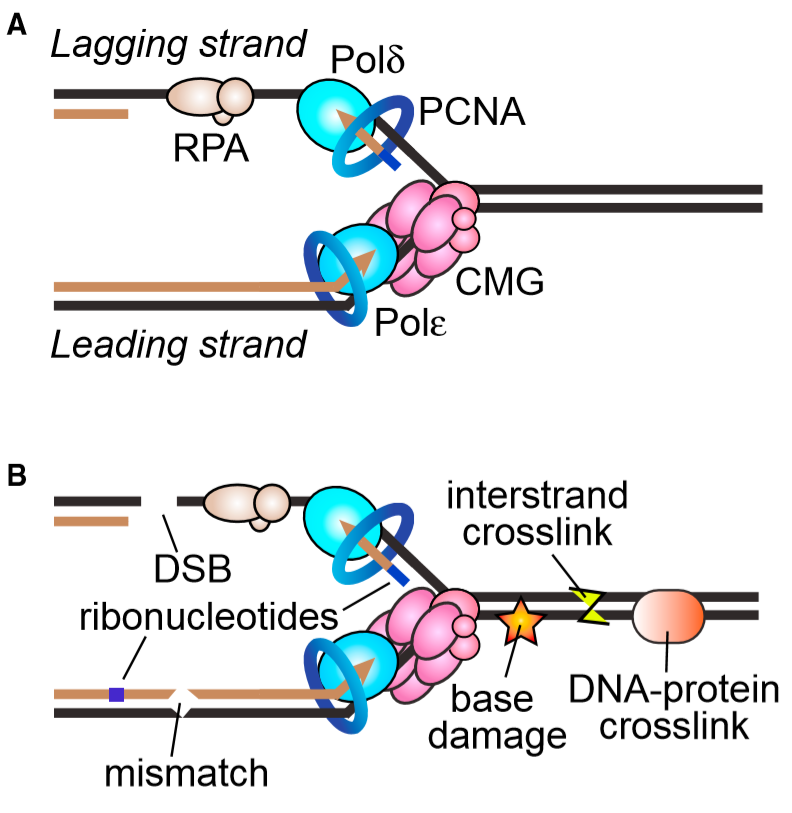
\includegraphics[width=0.56\textwidth]{resources/images/Intro/replicationfork.png}
    \caption[Resolution of DNA Lesions via Replication-Coupled Pathways]{\textbf{Resolution of DNA Lesions via Replication-Coupled Pathways.}\\A) Simplified schematic of a eukaryotic replication fork.\\B) Lesions generated or encountered by the replisome.\\\citep{Cortez.2019}}
    \label{fig:replicationfork}
\end{wrapfigure}
All of the syndromes briefly introduced above share an elevated risk for cancer though based on the inability to repair one or more types of DNA lesions which leads to genomic instability and/or uncontrolled growth of affected cells. Understanding the mechanisms of the repair of DNA lesions as well as the pathways regulating them is crucial for preventing cancer and treating syndromes such as the ones mentioned above. Though numerous studies have been published over the last decades that investigated and resolved the mechanisms behind the repair of individual DNA lesions there is no comprehensive resource available to researchers that focuses on DNA repair on a systemic level. Many proteins involved in the repair of DSBs are also associated with the repair of ICLs, even though lesion detection as well as regulation and recruitment of lesion specific proteins differs greatly between those mechanisms. Due to this we wanted to look at the interactions between each repair mechanism to resolve DNA repair as a system instead of a collection of individual pathways. To do so we applied graph theory to a collection of chromatin proteomic data investigating the recruitment of proteins involved in DNA repair and replication in \textit{Xenopus} egg extracts (see \ref{sec:extracts}) to specifically damaged DNA templates. Each of the sets used in this thesis has been - be it already published or still in progress - used to resolve or improve the understanding of a single repair mechanism but has never been comprehensively compared to experiments investigating other repair mechanisms. As will be explained in more detail in section \ref{sec:extracts} the \textit{Xenopus} egg extract systems have in the past only been used to investigate mechanisms that are dependent on replication of the DNA template used. Due to this most of this thesis will focus on replication coupled DNA repair mechanisms (see Figure \ref{fig:replicationfork}).

\subsection{DNA Replication and the Cell Cycle}
To understand how DNA lesions are repaired in a replication dependent manner, one has to understand DNA replication itself. Eukaryotic cells undergo different stages during their life cycle to ensure an efficient and error-free cell division that leads to the formation of two identical and functioning daughter cells. A key mechanism during this cycle is the replication of the genome and therefore the error-free synthesis of new DNA molecules based on a template. Before we go into detail about how replication is initiated and carried out, we want to give a short introduction to the cell cycle of eukaryotic cells and the differences between model organisms and humans.

\subsubsection{The Cell Cycle: A brief Overview}
The circular process of cell life and division is differently regulated for each type of differentiated cell, where some continue to divide indefinitely and others differentiate to the point of being fixed in one phase until cell death is induced. Figure \ref{fig:cellCycle} shows a schematic of the stages of the cell cycle. It consists of two mayor phases - M-Phase and Interphase - where the latter can be split into three main stages that make up the bulk of the cells life (see figure \ref{fig:cellCycle}). 
\begin{figure}
    \centering
    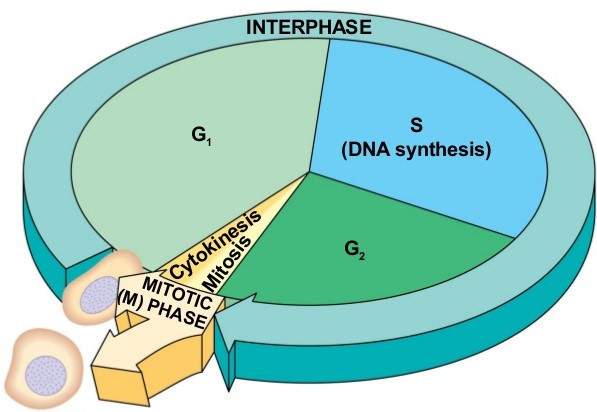
\includegraphics[width=.68\textwidth]{resources/images/Intro/cellCycle.jpg}
    \caption[Schematic view of the cell cycle]{\textbf{Schematic view of the cell cycle. }Cells experience 5 distinct phases during their life cycle. In G\textsubscript{1} the cell prepares to replicate its DNA in S-Phase and remains in G\textsubscript{2} until it has to divide its nucleus during mitosis. The cell cycle is completed after one maternal cell divides into two daughter cells during cytokinesis.\\\citep{Campbell.2015}}
    \label{fig:cellCycle}
\end{figure}
Simplified, Interphase starts with a stage called G\textsubscript{1} where all DNA is organised in a condensed form called heterochromatin that has to be unpacked to be replicated during the following S-stage. During S-phase DNA is replicated and the replicated molecules are attached to each other on their centromers to form so called sister-chromatids that are stored in the nucleus during the following G\textsubscript{2} phase. Differentiated cells that are not supposed to undergo mitosis anymore then enter G\textsubscript{0} until signalled otherwise or until cell death (not pictured in Figure \ref{fig:cellCycle}). 
Cells that are supposed to continue in cell division enter M-Phase which consists of Mitosis and Cytokinesis. During Mitosis, the nucleus of a cell is dissolved, the sister-chromatids are separated and transported to different poles of the cell. From there, two new daughter nuclei form to complete Mitosis. 
\begin{wrapfigure}{l}{0.4\textwidth}
    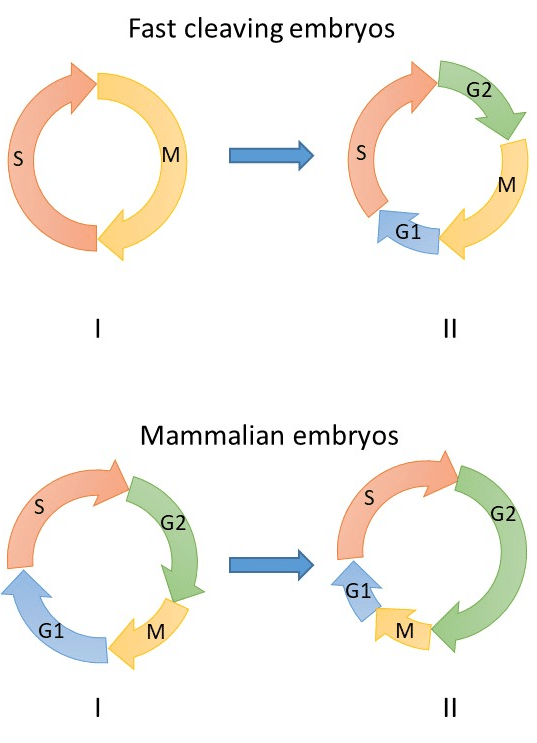
\includegraphics[width=.38\textwidth]{resources/images/Intro/cycleXenHum.png}
    \caption[Different course of fast cleaving VS. mammalian embryonic cell cycles]{\textbf{Different course of fast cleaving VS. mammalian embryonic cell cycles.}\citep{Kermi.2019}}
    \label{fig:XenHumCyc}
\end{wrapfigure}
Cytokinesis completes the cycle by dividing the cytoplasm of the mother cell into two newly generated daughter cells that enter Interphase. These Mechanisms are of course heavily regulated with molecular checkpoints that have to be cleared before entering a new phase. Additionally, regulatory proteins are deployed during S phase that inhibit DNA replication to prevent the cell from replicating its genome more than once. Such regulatory proteins can be used to induce stress in a cell or another system used to study replication and DNA repair (see section \ref{sec:extracts}).\\
Embryonic cell cycles show differences in the presence of phases and proteins in comparison to the cell cycle in adults as well as differences between classes of eukaryotes. Fast cleaving embryos such as \textit{Xenopus laevis} don't undergo G\textsubscript{1} and G\textsubscript{2} during Interphase in their early stages but show relatively short G-Phases and a longer M-Phase than mammalian embryos that start with all four phases and only change the duration of each phase during embryonic development (see Figure \ref{fig:XenHumCyc}).\\
All data used in this thesis was acquired using \textit{Xenopus} cell free egg extracts that can be used to study replication dependent mechanisms of DNA repair. Different extract types are used to study different mechanisms but the details of said extracts will be discussed later.

\subsubsection{Initiation of DNA Replication}
\label{sec:cellcycle}
The replication of DNA based on the template genome of a cell during S-Phase starts with the recruitment of the Origin Recognition Complex (ORC) consisting of six subunits to an Origin of Replication. Per DNA molecule, many origins are loaded with ORC but not all of them are activated. The mechanisms of choosing which origin stays dormant and which will get activated as well as the function of dormant origins is extremely complex and beyond the scope of this thesis. It has been shown that the dormant origins are involved in the maintenance of genomic stability \citep{Alver.2014}.
\begin{figure}[H]
    \centering
    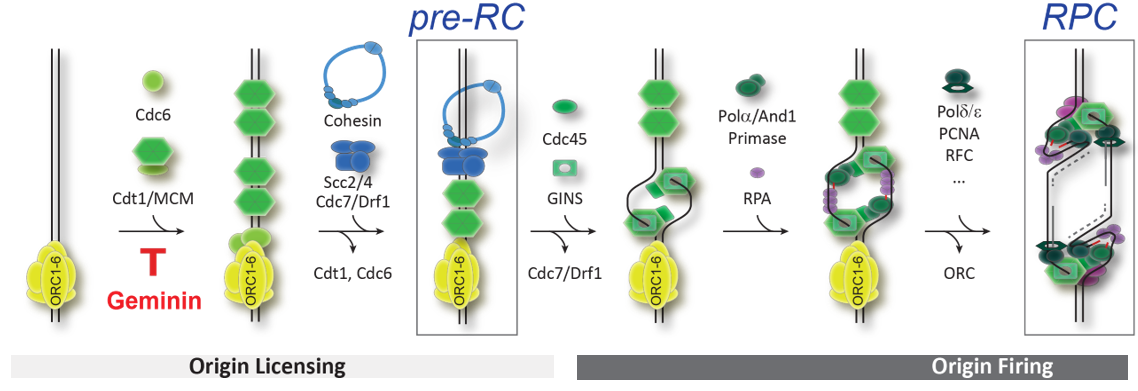
\includegraphics[width=\textwidth]{resources/images/Intro/repIni.png}
    \caption[Mechanisms of Replication Initiation]{\textbf{Mechanisms of Replication Initiation. } The origin recognition complex (ORC) binds to an origin of replication and recruits Cdc6 and the MCM-helicase that is associated with Cdt1. Cdt1 and Cdc6 dissociate from the origin to give way for the recruitment of the Scc2/4 Cdc7/Drf1 tetramer and Cohesins to complete the pre-Replication Complex (pre-RC). The Cdc7/Drf1 dimer is released and Cdc45 in conjunction with the GINS complex is recruited. With this, the origin  is prepared for DNA replication to be initiated. RPA, Primase and Pol\textalpha are then recruited and after release of the ORC other polymerases as well as PCNA are recruited to form the replication complex (RPC) and start replication.\\\citep{Raschle.2015}}
    \label{fig:replication_overview}
\end{figure}
Activated origins are then loaded with Cdc6 as well as the Cdt1/MCM complex. After dissociation of Cdt1 and Cdc6 the MCM helicase complex promotes recruitment of Cohesins and the Cohesin-recruiter proteins Cdc7 and Drf1 to form the pre-Replication Complex (pre-RC). The Cdc7/Drf1 dimer is replaced by Cdc45 and the GINS complex that bind to and activate the MCM helicase to open up the replication fork. DNA polymerases and the primimg protein Primase as well as the ssDNA stabilizing protein RPA are recruited to the now opened replication fork. To finalize the initiation of DNA replication PCNA is loaded and ORC dissociates from the origin. From there on each DNA molecule is replicated with an extremely low error rate until a potential DNA lesion is reached. each type of DNA lesion is detected by different factors and repair using specific molecular mechanisms that will be explained in the section below.\newpage

\subsection{An Introduction to the DNA Damage Response (DDR)}
Quick and accurate replication of DNA in each cell during every cell cycle is crucial for the survival of the cell. Even though the replisome is a very accurate machinery, it does not function error-free.\\\\
DNA replication is enabled by the use of three main polymerases: Pol\textalpha, which incorporates priming nucleotides, Pol\textdelta, which polymerizes the leading strand, and Pol\textepsilon, which polymerizes the lagging strand. These three polymerases are listed in order of descending error-proneness where Pol\textepsilon shows the highest fidelity with only 1 false base incorporations out of 10\textsuperscript{6} bases. 

\subsubsection{Resolution of Polymerase Blockages}
\label{sec:polblock}
Base lesions such as abasic sites, base oxidation and base methylation often pause polymerases in their path. Spontaneous base loss and glycosylase removal of uracil cause about 10,000 - 20,000 abasic sites each day in each human cell whereas all other base lesions form about 20,000 times each day on average. Environmental factors such as UV light can increase the rate of such base lesions dramatically and even though most of them are repaired by replication independent mechanisms such as Base Excision Repair (BER) or Nucleotide Excision Repair (NER), these systems can not always repair them prior to replication fork arrival.\\
The response to a base lesion heavily depends on the template strand the lesion is found in. A lagging strand lesion may stall Pol\textalpha-primase or Pol\textdelta but can not stall the replication fork in total because new primers on the lagging strand lead to a natural skippage of the lesion. The gaps created during those skipping maneuvers are repaired after replication by translesion-bypass polymerases. This lesion-skipping model has not yet been verified in vertebrates because of the difficulty of introducing lagging-strand directed lesions \citep{Goodman.2013}. Lesions on the leading strand however are block Pol\textalpha~more effectively because of the lack of new primers on the strand which leads to a functional uncoupling of the CMG helicase and the DNA synthesis. This uncoupling by itself may not be as problematic as one might expect. It has been shown in \textit{E. coli} that there is little coordination between leading and lagging strand synthesis with or without DNA damage. Additionally, helicase activity is reduced by ~80\% when DNA synthesis stops. This effectively forms a "dead man's switch" that prevents the helicase from unwinding too much DNA ahead of synthesis \citep{Goodman.2013,Marians.2018}. In case of the helicase running too far ahead, repriming of the leading strand occurs within several minutes and does not require a specific primase in \textit{E. coli} which allows replication to resume. The bacterial replisome is capable of skipping leading strand lesions relatively easily whereas the eukaryotic replisome has the ability to skip them to some extend but it seems to prefer usage of a specialized primase called \textit{PrimPol} \citep{Rechkoblit.2016}. An overview of the responses to leading- and lagging strand base damages can be seen in Fig. \ref{fig:lesionskipping}.
\begin{wrapfigure}{r}{0.6\textwidth}
    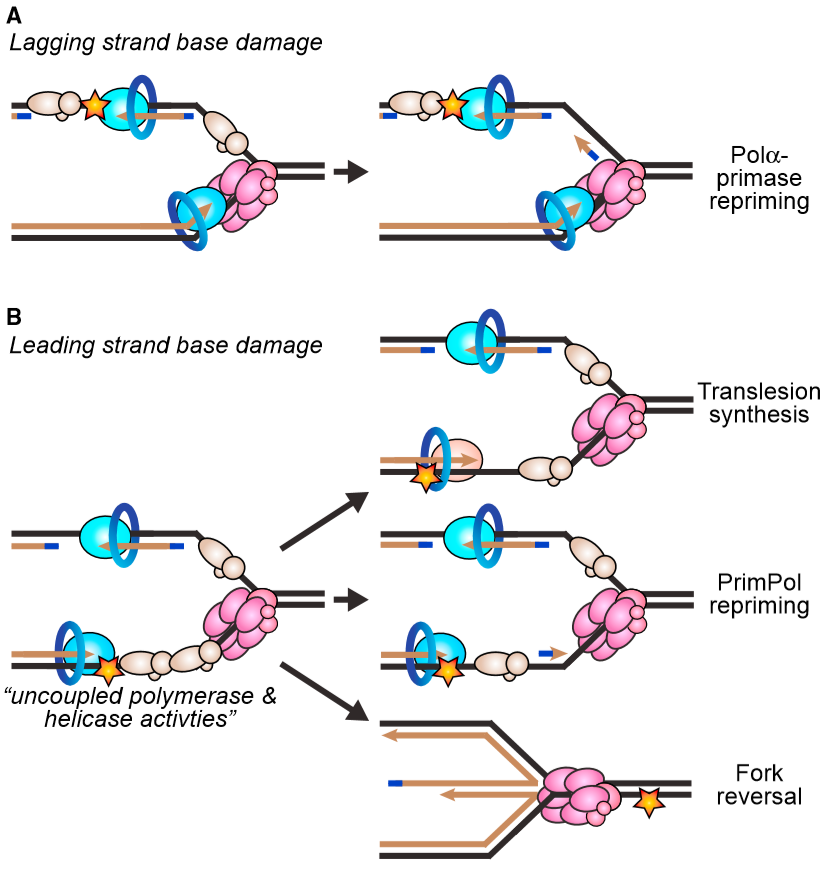
\includegraphics[width=0.58\textwidth]{resources/images/Intro/lesionskipping.png}
    \caption[Schematic of the Response to Leading- and Lagging Strand Base Damage]{\textbf{Schematic of the Response to Leading- and Lagging Strand Base Damage.}\\
    (A) Lagging strand base damages often create ssDNA gaps that can be repaired by Pol\textalpha-primase repriming. This does not block DNA elongation.\\
    (B) Leading strand base damages are repaired in one of three ways: Translesion synthesis,\textit{PrimPol} repriming or via Fork Reversal. Those three pathways help the resolution of DNA lesions that could otherwise lead to replisome uncoupling. \citep{Cortez.2019}}
    \label{fig:lesionskipping}
\end{wrapfigure}
Fork reversal has been described as an alternative to lesion skipping. This mechanism is catalyzed by enzymes including SMARCAL1 (also called HARP), ZRANB3 and HLTF \citep{Betous.2012, Kile.2015}. Fork reversal happens by migrating the three-way fork junction backwards to anneal nascent DNA strands while forming a so called chicken foot structure (Fig. \ref{fig:lesionskipping}B and Fig. \ref{fig:forkreversal}).

Around 25\% of all fork defects caused by nucleotide depletion, oxidative base damage, DNA crosslinks and UV photoproducts are resolved by this mechanism \citep{Zellweger.2015}. Inactivating one of the mentioned key enzymes changes the cells replication stress sensitivity and alters fork progression while genomic stability is reduced \citep{Ciccia.2010, Yuan.2009}. Due to this, fork reversal is now seen as an essential part of effective DNA replication and repair even if the replisome encounters lesion that should be easy to skip. One potential benefit of fork reversal is the placement of template DNA lesions into the context of duplex DNA to enable excision repair mechanisms to function properly. Although there is little data that suggests a coupling of excision repair to fork reversal, one possibility shown by \citet{Weston.2012} is the involvement of ZRANB3 in the removal of DNA lesions due to its endonuclease domain in addition to its fork-remodeling functions. Additionally, fork-reversal is an essential part of repair mechanisms involved in the convergence of two forks on an interstrand crosslink as well as an intermediate in a recombination pathway of fork restart \citep{Amunugama.2018}.
\begin{wrapfigure}{l}{0.6\textwidth}
    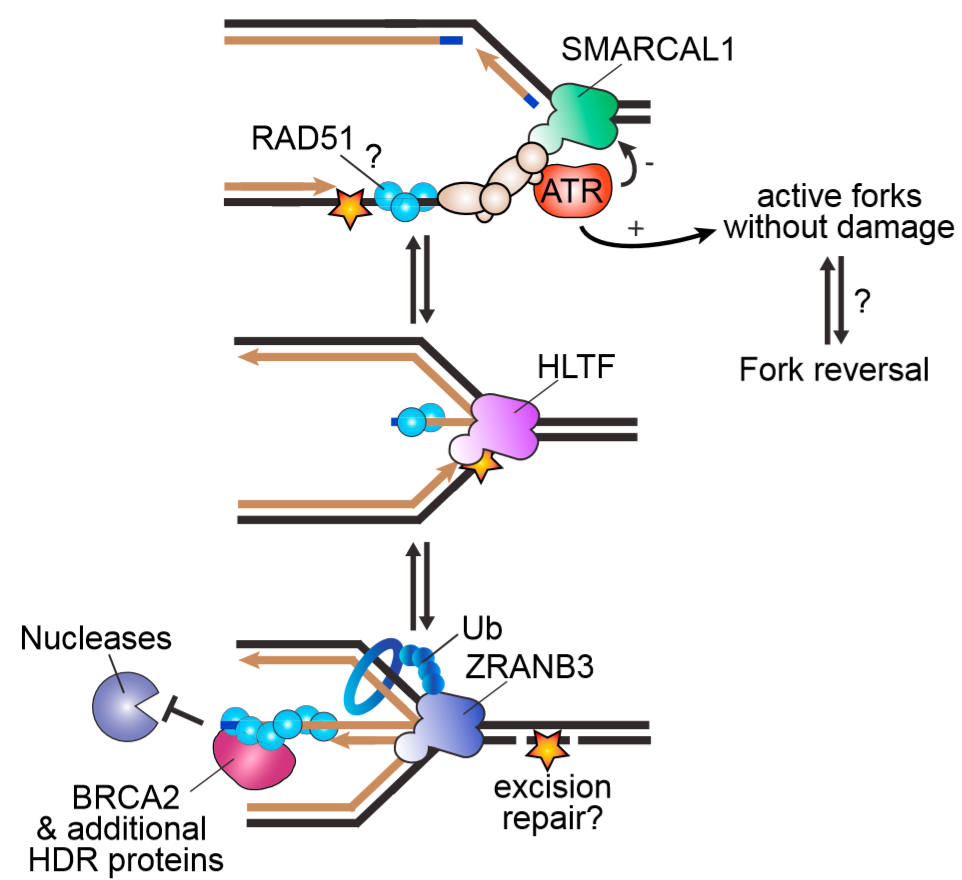
\includegraphics[width=0.56\textwidth]{resources/images/Intro/forkreversal.PNG}
    \caption[Schematic of Fork-reversal]{\textbf{Schematic of Fork-reversal.} Through fork reversal the damaged simplex DNA is placed back into a duplex context where the damage can be removed via excision repair. SMARCAL1, HTLF and ZRANB3 are regulated by RPA, 3' DAN ends and poly-ubiquitylated PCNA (see below) respectively. \citep{Cortez.2019}}
    \label{fig:forkreversal}
\end{wrapfigure}
Recombination proteins such as RAD51, BRCA1 and BRCA2 play crucial roles in fork-reversal pathways. \cite{Neelsen.2015} proposed that RAD51 binds ssDNA on the template strand start a coordinated annealing reaction (see Fig. \ref{fig:forkreversal}). \cite{Bhat.2018} on the other hand published some evidence on RAD51 capturing nascent ssDNA  as its formed by recombination proteins to shift the equilibrium towards fork-reversal.\\
Reversed forks aren't static constructs but can rather be processed by Double-Strand-Break repair nucleases like MRE11 or DNA2. Processing by those nucleases may remove end-binding proteins and therefore promote fork restart \citep{TeixeiraSilva.2017}. It has been shown that the MRE11-RAD50-NBS1 (MRN) nuclease binds to replication forks even in absence of exogenous DNA damage to interact with RPA but end-processing is mostly restricted by RAD51 to prevent nascent strand degradation \citep{Mijic.2017, Dungrawala.2015}. The actual actions of RAD51 at forks are heavily regulated by proteins including BRCA1, BRCA2 and the FANC proteins. The mentioned proteins promote RAD51-dependent fork protection but are not essential for fork-reversal. Negative regulation of RAD51 is done through RADX, FBH1 and BLM, indicating that repair mechanisms must not only be activated to act on specific lesion but they also need to be negatively regulated to prevent some effects of over-repair that can actually be more deleterious than the initial lesion \citep{Bhat.2018}.\\
The exact fate of the replication machinery during fork-reversal is not clearly known but there is some evidence for the dissiciation of the replisome \citep{Dungrawala.2015} whereas the CMG helicase most likely remains on the fork. This can be assumed due to the competence of most forks to resume replication quickly after prolonged blockage.\\\\
Fork reversal and lesion skipping may be independent mechanisms that could operate individually. How mammalian cells choose between the two pathways is not well studied yet. Post-translational modifications like ubiquitylation and sumoylation, especially to PCNA, are essential in pathway choice. ATR signalling also seems to play a critical role because reversal enzymes like SMARCAL1 are ATR substrates. Phosphorylation of SMARCAL1 by ATR for example has been shown to reduce its fork-remodelling activity \citep{Couch.2013}. \cite{Mutreja.2018} report an ATR-promoted stalling of forks that have not encountered any lesions by signalling from stalled forks.How exactly the reversal of undamaged forks benefits the cell even though it delays the completion of DNA replication is unknown.

\subsubsection{Resolution of Helicase-Blocking Lesions}
\label{sec:iclrepair}
Interstrand Crosslinks (ICLs) and DNA-Protein Crosslinks (DPCs), especially on the leading strand, pose a potent risk of fork blocking because they interfere with helicase unwinding, although they are much less common than polymerase-blocking lesions.\\
As already mentioned ICLs are formed in response to DNA-damaging agents that are used in cancer chemotherapy, such as Psoralen and mitimycin C, as well as through ionizing and UV radiation. Many effectors that can cause ICLs also cause DPCs. Additionally, interrupting the catalytic cycle of DNA-binding enzymes can lead to protein-DNA intermediates. Removal of those lesions by replication-coupled repair mechanisms is done through three main pathways.\\
One might expect complete blockage of replication fork movement in response to an ICL or DPC, but that is not the case. The CMG helicase encircles the leading strand and uses MCM10 as an accessory protein that helps to prevent lagging strand DPCs from blocking the helicase \citep{Langston.2017}. DPCs on the leading strand, that are be to big to physically be accommodated by the CMG channel, can also be traversed by the helicase via unwinding of DNA past the lesion by the accessory polymerase RTEL1 to provide a short ssDNA strand. This allows the MCM complex to bypass the DPC which promotes proteolysis-dependent repair of said lesion \citep{Sparks.2019}.\\
\begin{figure}[H]
    \centering
    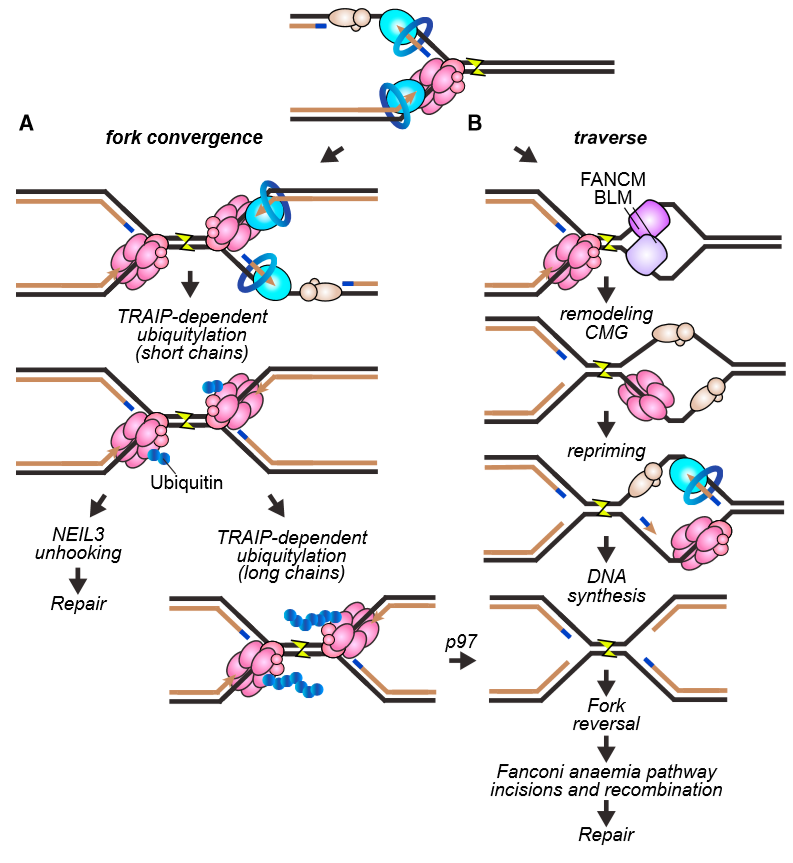
\includegraphics[width=0.7\textwidth]{resources/images/Intro/icl_replication.PNG}
    \caption[Replication-Coupled ICL Repair Mechanisms]{\textbf{Replication-Coupled ICL Repair Mechanisms.}\\
    A) Forks converge on an ICL, TRAIP-dependent short-chain ubiquitylation promotes recruitment of NEIL3 and leads to strand-unhooking. Long-chain ubiquitylation leads to unloading of the replisome followed by fork reversal and DNA incision via the Fanconi anemia pathway.\\
    B) ICL traversion via the use of FANCM and BLM as accessory helicases. Remodeled CMG helicase may allow traversal of the lesion followed by repriming of the MCM complex past the lesion. This leads the ICL to be repaired post-replicatively via the Fanconi anemia pathway.\\
    \citep{Cortez.2019}}
    \label{fig:iclrepl}
\end{figure}
ICLs also do not block the CMG helicase completely. The two additional helicases FANCM and BLM as well as the ATR kinase and FANCD2 can remodel the CMG helicase \citep{Huang.2013} in a way that allows "traversal" of interstrand corsslinks, although exact mechanisms for this have not been resolved yet \citep{Huang.2019}. The general mechanism of ICL traversal is similar to that of DPC traversal in that the CMG helicase may be blocked from unwinding DNA, but as long as another helicase provides ssDNA the MCM complex can reform past the lesion. Interestingly, ICL traversal can not be observed in \textit{Xenopus} egg extract systems which may be due to the high concentration of replication proteins that could disfavor ICL traversion.\\
DPC and ICl traversion lead generally to a similar situation to a base lesion which means that polymerases are stalled while the CMG helicase is able to continue unwinding DNA.Therefore repair of said ICL has to occur post-replicatively.  A DPC would not be lethal on its own wheras ICLs could interfere with chromosome segregation causing mitosis errors and cell death. Figure \ref{fig:iclrepl} shows possible replication-coupled mechanisms for ICL repair.\\\\
The two described possibilities for ICL handling during replication both end in X-shaped DNA structures around the crosslinks (see Fig. \ref{fig:iclrepl}). Unhooking of the crosslink is essential to complete replication and chromosome segregation and takes place through at least two independet pathways.\\
\begin{figure}[H]
\centering
    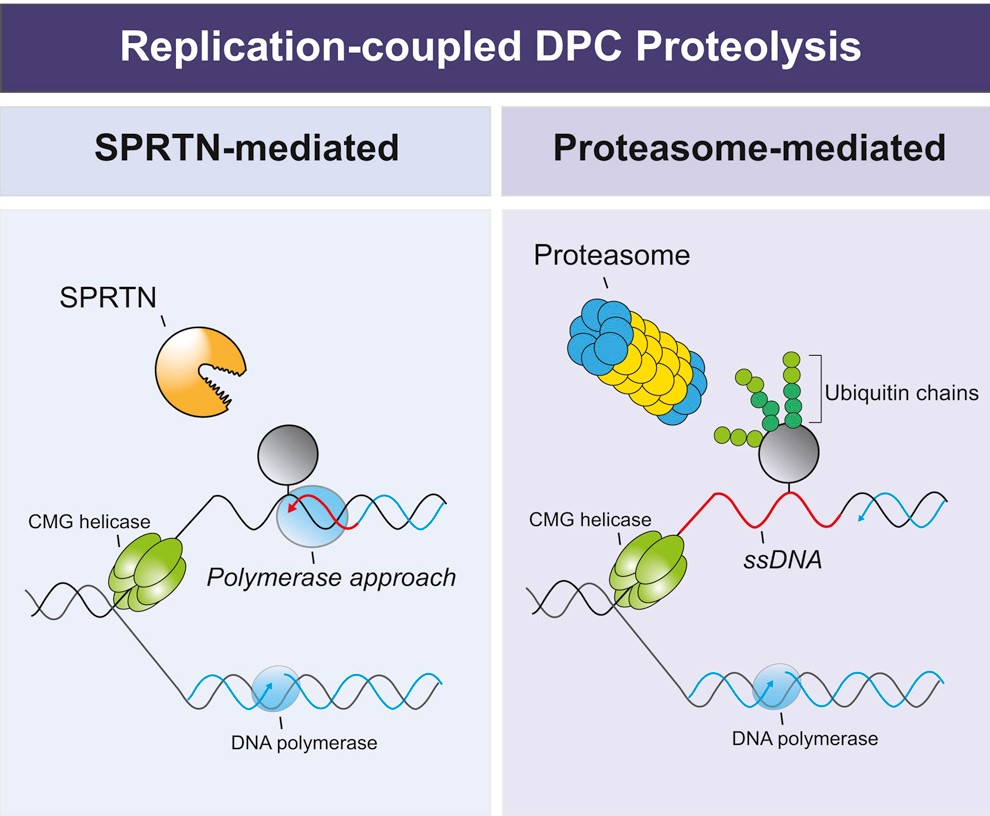
\includegraphics[width=.68\textwidth]{resources/images/Intro/sprtn.jpg}
    \caption[SPRTN- and Proteasome-mediated DPC Proteolysis]{\textbf{SPRTN- and Proteasome-mediated DPC Proteolysis.} SPRTN recognizes polymerase stalling on both the leading and the lagging strand and mediates DPC proteolysis similar to the yeast protease Wss1 \citep{Stingele.2015}. Proteasome-mediated proteolysis requires polyubuquitylation of the DPC.\\ \citep{Larsen.2019}}
    \label{fig:sprtn_action}
\end{figure}
Psoralen- and abasic site induced ICLs are mostly unhooked without DNA incision through NEIL3 \citep{Semlow.2016}. Unhooking via the NEIL3 glycosylase leaves an abasic site on one template strand and a mono-adduct or adenosine on the other. Those lesions are then repaired via TLS and some additional steps \citep{Raschle.2015}. Lesions introduces via other effectors are not good substrates for NEIL3 and have to be repaired via an alternative pathway involving a FANC protein-dependent mechanism. The FANC proteins get their name from the disorder that arises when one or more are inactivated called Fanconi anemia, that is characterized by cellular hypersensitivity to crosslinking agents \citep{Ceccaldi.2016}. This pathway requires the CMG helicase to be unloaded , the DNA backbone to be incised as well as the involvement of fork reversal \citep{Amunugama.2018}. Initially it was thought that BRCA1 was required for CMG helicase unloading but new evidence suggests that TRAIP catalyzes CMG ubiquitylation and therefore promotes p97-dependent unloading \cite{Wu.2019}.\\
DPC repair also requires further processing after lesion-traversion but because large DPCs block NER, at least two proteolysis-dependent mechanisms are required to resolve such lesions. Both of those mechanisms rely on SPRTN or the proteaseome \citep{Stingele.2016,Vaz.2016}.\\
Ubiquitylation of DPCs catalyzed by the E3 ligase TRAIP is neccessary to trigger proteasome activation. Sumoylation also regulates DPC repair but it is not well understood how nearby DNA-binding proteins are protected from proteasomal removal. Once proteasomal degradation is finished, the remaining small-peptide-crosslink can be excised by NER after the gap in the daughter strand is closed by a combination of Pol\textdelta~ and TLS polymerases. Because of this DPC repair via the proteasome is considered to be mutagenic.\\ An additional mechanism of DPC proteolysis has been described to be mediated by the metalloprotease SPRTN in eukaryotes \citep{Gao.2018}. SPRTN has been shown to act in a similar way to the yeast protease Wss1 \citep{Stingele.2015} meaning it recognizes polymerase stalling on both the leading and the lagging strand without the need for polyubiquitylation of the DPC the fork is stalling at \citep{Larsen.2019}.   
There is a possibility of topoisomerase proteins not completing their catalytic cicle which leads to them staying covalently bound to the DNA. Drugs like etoposide are considered topoisomerase poisons and greatly increase the frequency of such covalent bounds occuring. \cite{Pommier.2014} showed that those topoisomerase-DNA complexes are removed by tyrosyl-DNA phosphodiesterases (TDP1 or TDP2) that are regulated via ubiquitylation and sumoylation.

\subsubsection{Double Strand Break (DSB) Repair during replication}
Breaks in the DNA backbone are generated via multiple mechanisms during replication where any process that involves strand cutting can introduce DSBs. They can also be caused by structure-specific nucleases such as MUS81 that process persistently stalled forks \citep{Hanada.2007}.\\
In stark contrast to DSBs that form in cells in G\textsubscript{0} or G\textsubscript{1} phase, replication-associated breaks are mostly "single ended" in nature, meaning that recombination is the preferred mechanisms to resolve them. Breaks in the DNA strands caused during replication can be repaired using a process called Break Induced Replication (BIR) where a DNA resection followed by strand invasion can generate a fork structure that is capable of DNA synthesis using a modified replisome \see Figure \ref{fig:bir}.
\begin{figure}[H]
    \centering
    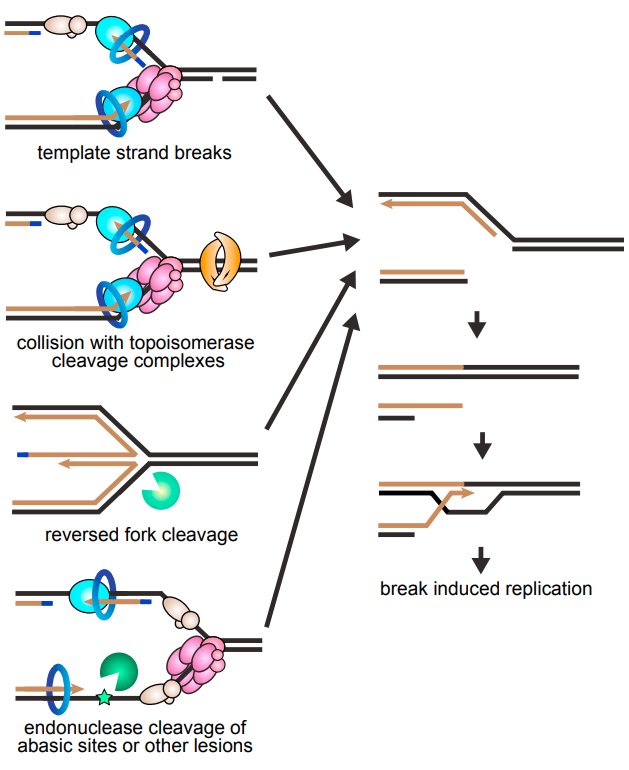
\includegraphics[width=.65\textwidth]{resources/images/Intro/bir.PNG}
    \caption[Mechanisms of DSB generation at Replication Forks]{\textbf{Mechanisms of DSB generation at Replication Forks. }Single-ended breaks are repaired by break-induced replication. The individual mechanisms depend heavily on an alternative replisome.\\\citep{Cortez.2019}}
    \label{fig:bir}
\end{figure}
BIR in general is best understood in yeast systems but has been studied in every eukaryotic organisms as well as in model system such as \textit{Xenopus} egg extracts. As a mechanisms involving strand invasion RAD51 plays a major role in BIR as well as an additional subunit of Pol\textdelta called POLD3 in humans or Pol32 in yeast. RAD51-dependent BIR mechanisms always involve RAD52 and are engaged at extraordinarily fragile sites. One example of this is when during replication MUS81 cleaves unreplicated DNA during mitosis. This underlines the idea that BIR is a mechanisms to prepare for mitosis and to facilitate chromosome segragation \citep{Bhowmick.2016}. Finally, BIR can be useful for telomere extension in cells using ALT where telomere damage induces a BIR replisome to replicate telomere sequences \citep{Dilley.2016}.

\subsubsection{Mismatch Repair}
Misincorporation errors are mainly repaired by mismatch repair (MMR). Base mismatches can by definition only occur on the daughter strand, therefore it is necessary to reliably distinguish the template from the daughter strand. In \textit{Escherichia coli} the template strand has a specific methylation pattern in the palindromic repeat sequence d[GATC] This enables excision and replacement of mismatched nucleotides  directed by the detection of a nick on the daughter strand caused by an error in this pattern \citep{Kunkel.2005}.\\
Similarly in eukaryotes, specifically in eukaryotic cell free extracts, mismatch repair is directed by a nick located 3' or 5' to the mismatch. The rate of mismatch repair is inverse proportional to the distance between the nick and the error from 125 to 1000 bp although repair was shown at much larger distances \citep{Iyer.2006}.\\
The actual repair of mismatched nucleotides is mediated by the redundant heterodimer MSH6-MSH3 that detects smaller insertion/deletion loops (IDLs) of 1-2 bp in cooporation with their obligate partner MSH2 whereas larger IDLs are detected by MSH2-MSH3. In addition to that MSH6-MSH3 interact with the DNA polymerase processivity factor proliferating cell nuclear antigen (PCNA) to localize MMR heterodimers to replication forks to repair replication errors as they occur. When MSH6-MSH3 encounters a DNA mismatch it undergoes a conformational change to a sliding clamp that diffuses along the DAN to free up mismatched nucleotides for recognition via MSH2-MSH6. This dimer recruits the heterodimer MLH1-PMS2 which in turn regulates the loading of the exonuclease Exonuclease 1 (Exo1) onto the daughter strand to promote excision of error-containing DNA fragments \citep{Gupta.2019}.
\newpage

\subsection{\textit{Xenopus} egg extracts as a Model System for Chromatin Proteomics}
\label{sec:extracts}
Studying proteins bound to chromatin is a crucial part of understanding the systemic and molecular mechanisms of DNA Repair and Replication. Even though systems like \textit{Xenopus} egg extracts have been used for decades to study different aspects of DNA processing using more traditional methods such as Western Blots and Immunostaining, the rise of mass spectrometry gave way to the field of high-throughput chromatin proteomics \citep{Blow.1990,Cupello.2016,Bonisch.2008}. One study that should be mentioned in the context of \textit{Xenopus} egg extracts in mass spectrometry is the large collaborative effort of M. Räschle, J. C. Walter, Z. Storchov\a'\ and M. Mann published in 2015 \citep{Raschle.2015} that explained how DNA crosslinks are detected and repaired using protein-chromatin interaction networks to resolve protein modules involved in crosslink repair.
\begin{figure}[H]
    \centering
    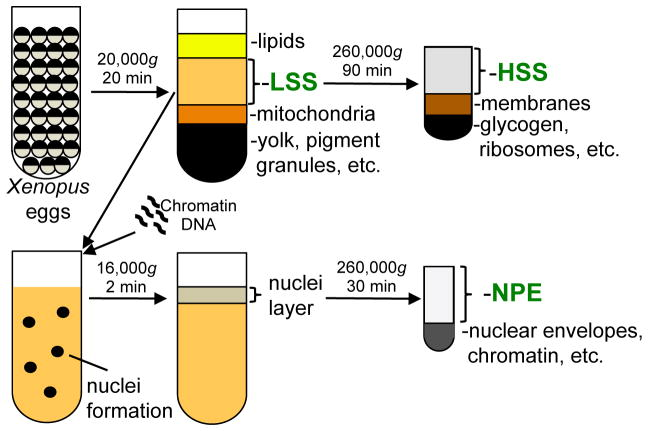
\includegraphics[width=.78\textwidth]{resources/images/Intro/extracts.jpg}
    \caption[\textit{Xenopus} egg extracts]{\textbf{\textit{Xenopus} egg extracts.} \textit{Xenopus} eggs are packed and then centrifuged at 20.000g for 20 min to separate lipids, mitochondria and yolk from the Low Speed Supernatant (LSS). Centrifugation of LSS at 260.000g for 90 min isolates the High Speed Supernatant (HSS) from the membranes and ribosomes. The addition of chromatin DNA to LSS leads to the formation of nuclei that can be separated from the rest of the mixture via a short centrifugation at 16.000g. An additional high speed centrifugation of the nuclei layer at 260.000g for 30 min separates the Nucleoplasmic Extract (NPE) from the nuclear envelops and the added chromatin.\\\citep{Cupello.2016}}
    \label{fig:extracts}
\end{figure}
\newpage
There are three main ways to prepare cell free extracts from \textit{Xenopus} eggs that are used to study specific aspects of chromatin processing. The easiest extract system to prepare is the so called Low Speed Supernatant (LSS) where eggs are packed and then centrifuged. This separates a yellow-brown mixture of protein, glycogen and membranes, the LSS extract, from the rest of the egg. Centrifuging LSS at high speeds separates the so called High Speed Supernatant (HSS) from membranes, glycogen and ribosomes. 
\begin{figure}[H]
    \centering
    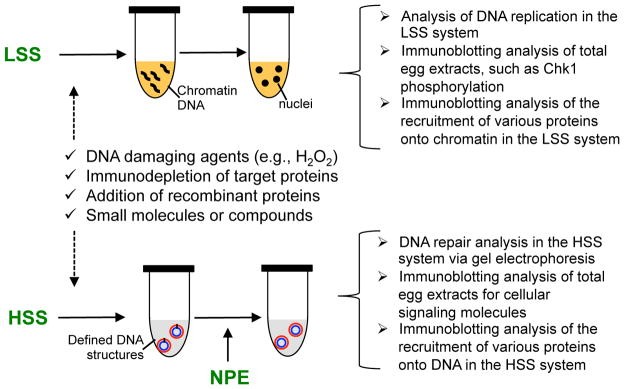
\includegraphics[width=.88\textwidth]{resources/images/Intro/extracts_uses.jpg}
    \caption[Usecases for \textit{Xenopus} egg extracts]{\textbf{Usecases for \textit{Xenopus} egg extracts.} Mixing LSS with chromatin DNA leads to the formation of nuclei that can be used to analyze DNA replication, for immunoblotting of total extracts and for proteomic analysis of protein recruitment to chromatin. Addition of substrate DNA to HSS forms the pre-replication complex (pre-RC) and licenses the added substrate for replication. After adding NPE DNA repair mechanisms can be analyse via gel electrophoresis while it is also possible to investigate protein recruitment and modification via proteomic methods.  \\\citep{Cupello.2016}}
    \label{fig:extract_uses}
\end{figure}
These extract systems deliver reliable tools to scientists studying the mechanisms of DNA repair and replication in a eukaryotic system that is closer to that of humans than fungal systems such as yeast, even though the molecular composition of the \textit{Xenopus} extract systems are not equal to unobstructed cells due to the treatments necessary for preparation. What extract system to choose for the experiment one wants to conduct depends heavily on these molecular differences and will be subject of later parts of this introduction (see Section \ref{sec:chromass} and \ref{sec:pp-ms}). As an example it should be mentioned that LSS as the simplest extract system is molecularly comparable to the embryonic interphase until sperm chromatin is added which initiates replication and therefore moves the extract to S-Phase (see Figure \ref{fig:cellCycle}.\\\\
In studies looking at the replication stress response of egg extracts LSS was treated with the endogenous regulatory protein Geminin which is synthesized during S phase to inhibit DNA replication by binding the initiation factor Cdt1 that cooperates with the ORC (origin recognition complex, \cite{Cook.2004}) to form the pre-RC complex (see section \ref{sec:cellcycle}.
\begin{figure}[H]
    \centering
    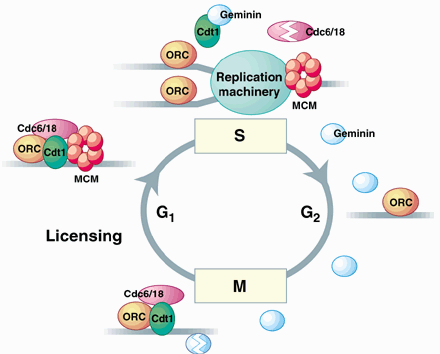
\includegraphics[width=.78\textwidth]{resources/images/Intro/gemininCell.png}
    \caption[Schematic depiction of a cell cycle showing the action of Geminin.]{\textbf{Schematic depiction of a cell cycle showing the action of Geminin. } During S phase once DNA replication started the regulatory protein Geminin is expressed. Geminin binds to Cdt1 and therefore inhibits the formation of the pre-RC to prevent the replication of already replicating DNA molecules. Geminin expression is kept up throughout G\textsubscript{2} but is decreased in M to allow effective chromatin licensing in G\textsubscript{1}. \citep{Lygerou.2000}}
    \label{fig:geminin}
\end{figure}
Even though HSS and NPE are essentially different extracts, they have to be mixed to study replication-dependent mechanisms due to the fact that HSS mostly contains proteins neccessary to form the pre-RC complex and NPE does not. Without the addition of HSS to NPE DNA replication can not start because no origin licensing can occur (\cite{Lebofsky.2009} and Figure \ref{fig:replication_overview}). 
Therefore they can be considered as one system --- referenced henceforth as the NPE/HSS system --- even though non-replicating extracts are rising in popularity due to the possibility to study replication-independent repair mechanisms as well as interaction of different ATPases with DNA (unpublished studies, J.C. Walter \& M. Räschle).

\subsubsection{CHROmatin MASS Spectrometry}
\label{sec:chromass}
The CHROMASS (Chromatin Mass Spectrometry) system established by \cite{Raschle.2015} uses \textit{Xenopus} egg extracts described in \ref{sec:extracts} to analyse chromatin bound proteins using mass spectrometry. CHROMASS can therefore be used to analyse the time-dependent recruitment of proteins to chromatin under different conditions to characterize repair- and replication mechanisms.
\begin{figure}[H]
    \centering
    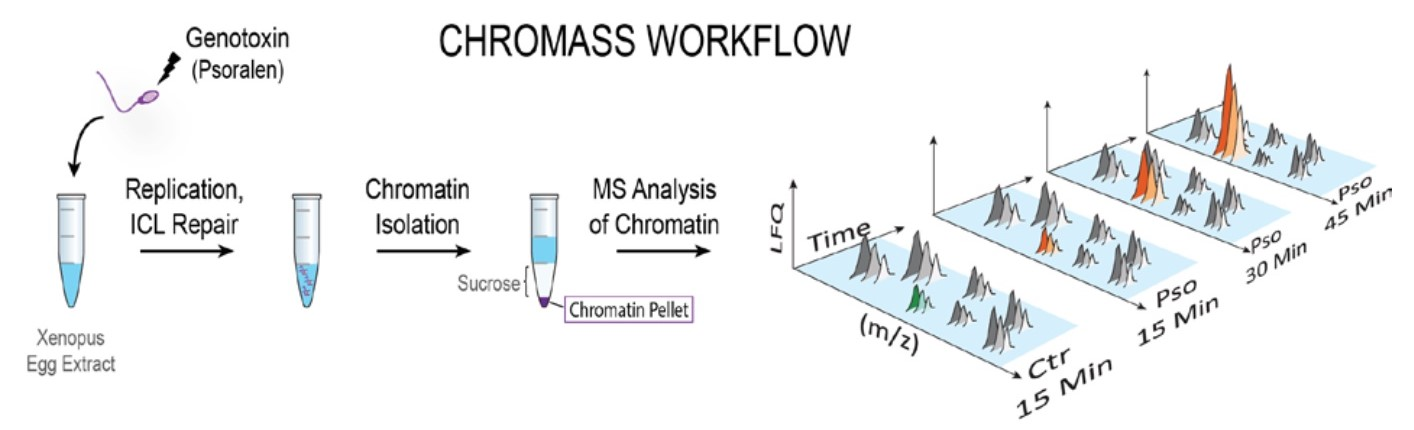
\includegraphics[width=0.98\textwidth]{resources/images/Intro/chromass.PNG}
    \caption[CHROMASS workflow.]{\textbf{CHROMASS workflow.} Genotoxin-treated sperm chromatin is added to \textit{Xenopus} egg extracts to initiate replication and repair. Chromatin is isolated after incubation for 15, 30 and 45 min via centrifugation through a sucrose cushion. The proteins bound to chromatin are isolated, digested, desalted and measured via mass spectrometry.\\ \citep{Raschle.2015}}
    \label{fig:chromass}
\end{figure}
Figure \ref{fig:chromass} shows the workflow used by \cite{Raschle.2015} to characterize the dynamic complex assembly during ICL bypass. Generally, damaged or undamaged sperm chromatin is added to \textit{Xenopus} egg extracts and then kept at room temperature (RT) to initiate replication and repair of added DNA. The chromatin is then separated from the mixture after set time points after initial addition by centrifuging through a sucrose cushion. Chromatin-bound proteins are then purified and a tryptic digest followed by a desalting step are performed. The purified peptides are then measured via mass spectrometry. For this kind of study, all of the three extract systems described in section \ref{sec:extracts} can be used to study protein recruitment in a time-dependent manner. MS DATA LOOKS LIKE TRADITIONAL RESULTS --> CHROMASS WORKS!

\subsubsection{Plasmid-Pulldown Mass Spectrometry}
\label{sec:pp-ms}
\begin{wrapfigure}{r}{.5\textwidth}
    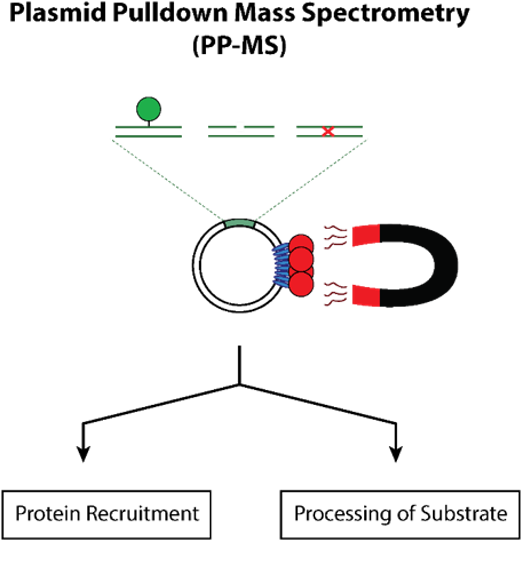
\includegraphics[width=.48\textwidth]{resources/images/Intro/pp-ms.png}
    \caption[Plasmid-Pulldown Mass Spectrometry workflow]{\textbf{Plasmid-Pulldown Mass Spectrometry workflow.}The plasmid substrate contains defined lesions and multiple repeats of a \textit{lacI}-binding sequence. After incubating the reaction mixture for the desired time a defined volume is removed and combined with beads coupled to \textit{lacI} which binds the plasmid substrate and therefore all DNA-bound proteins. The beads are then processed for mass spectrometry or loaded onto gels to visualize substrate processing (modified, Markus Räschle).}
    \label{fig:pp-ms}
\end{wrapfigure}
Plasmid-Pulldown Mass Spectrometry (PP-MS) is a system closely related to CHROMASS, although it has been shown that only the NPE/HSS system reliably replicates the plasmid DNA used for this method. Generally, plasmids with defined lesions are added to NPE/HSS and incubated to allow replication and repair. Isolation of this template DNA is achieved via a pull-down system which is enabled by the inclusion of a \textit{lacI}-binding site on the plasmid. The reaction mixture is added to \textit{lacI}-coated beads that bind to the \textit{lac}-operon fragment on the plasmid. The mixture is washed multiple times to remove unbound molecules after which the beads were dried and prepared for mass spectrometry in a similar fashion to the methods described in section \ref{sec:chromass}.\\
In addition to the proteomic analysis PP-MS can also be used to process the substrate DNA via gel electrophoresis to visualize replication kinetics (Fig. \ref{fig:pp-ms}).\\ 
This system has recently been used to describe the mechanism of SPRTN- and Proteasome-mediated replication-dependent DNA-Protein crosslink repair in \textit{Xenopus} egg extracts \citep{Larsen.2019}. The main benefit of PP-MS over CHROMASS is the ability to create specific lesions on the substrate in comparison to mostly unspecific lesion on sperm chromatin treated with genotoxins. Additionally, the repair of the lesion takes place over a shorter time-frame because plasmid DNA has a significantly faster replication kinetic due to its structure and size and its independence of prior chromatin assembly in \textit{Xenopus} egg extracts \citep{Sanchez.1992, AquilesSanchez.1995}. Using protein binding motifs on the plasmid templates it is also possible to synchronize their replication.\\

\subsection{Big Data and Networks in Biological Research}
Methods such as the ones described in the sections above create large amounts of data that have to be processed and handled correctly. Big Data, as the aggregate of such large datasets tends to be called, is used to draw conclusions from individual collections of data as well as the entirety of those collections.\\
Advanced computational methods such as the ones used by NCI in the development of TCGA can help understand biological systems using data gathered by 'omics experiments such as CHROMASS or PP-MS. Identification of key regulatory factors and mechanisms is crucial in resolving those systems and can be directly achieved by for example co-expression analysis in the case of gene expression data. Co-expression analysis algorithms can also be applied to  CHROMASS and PP-MS data sets under the assumption that proteins found on chromatin are recruited to it under specific conditions. This enables one to identify functionally similar proteins due to their similar chromatin binding pattern. The similarity of data collected for different proteins in one or more experiments can then be visualized in form of a protein-protein or gene co-expression network.
\subsubsection{Network visualization using correlation algorithms}
The following section is based on \cite{Dytham.2011} unless specified otherwise.\\\\
A relatively simple way to tackle co-expression analysis is correlation which is a measure of the relationship between two variables. Pearson's r correlation is the most widely used correlation statistic to measure the degree of relationship between variables that are linearly related. Pearsons correlation coefficient $r$ is calculated using the following equation.\\
\begin{equation}
    r_{xy} = \frac{n\sum x_i y_i - \sum x_i \sum y_i}{(\sqrt{n\sum x_i^2-(\sum x_i)^2}\sqrt{n\sum y_i^2-(\sum y_i)^2}}
\end{equation}
$r_{xy}:$ Pearson r correlation coefficient between $x$ and $y$\\
$n:\text{number of observations}$\\
$x_i:\text{value of $x$ (for ith observation)}$\\
$y_i:\text{value of $y$ (for ith observation)}$\\
\\
Pearson correlation only works based on the assumption that both variables are normally distributed and have a linear relationship. Additionally, the data has to be homoscedastic meaning it has to be equally distributed along the regression line. Given these assumptions Pearsons $r$ can be useful to investigate biological mechanisms up to more complex relationships such as protein-chromatin interaction networks.\\
The calculated correlation matrix for a set of variables can then be visualized in form of a network where the nodes represent variables and the edges their relationship. Additionally it is possible to use grouping algorithms such as Hierarchical Clustering to look at especially highly correlating variables.\\
To minimize computational effort and to reduce noise in the data set it is necessary to filter the gathered correlation matrix by the coefficient as well as the p-value. Determining the thresholds for filtering is another challenge in itself that can be tackled in different ways.\\
The simplest and most dangerous method of filtering networks for ease of visualization is setting a fixed correlation threshold. This is known as \textit{hard thresholds} where all edges of the network are filtered in such a way that all edges with $x \geq \tau$ are included. This method produces simple results that come with the danger of losing meaningful information depending on the threshold. If one sets $\tau = 0.7$ it is possible to lose a meaningful edge that has a weight of $0.6985$ \citep{Carter.2004}.\\
Another option is filtering for statistical significance of the calculated correlation coefficient based on the assumption that they are normally distributed meaning that the probability density function follows:\\
\begin{equation}
    f(x)=\frac{1}{\sigma \sqrt{2\pi}}e^{-(x-\mu)^2/2\sigma^2}
\end{equation}
$\sigma:\text{standard deviation}$\\
$\mu:\text{mean}$\\
\\
The p-value itself describes the probability of obtaining test results that are at least as extreme as the actually achieved results, meaning that it tells one if an observation could have also been done at random. An observation can be seen as statistically significant if $p < 0.05$ and highly significant if $p < 0.01$, stating that the probability making said observation at random is below 5\% or 1\% respectively.
For Pearson's $r$ this can be done relatively easily because the p-value for this measure of correlation uses the t-distribution. In this case $H_0:p=0$ vs. $H_1: p\ne0$ where $p$ is the correlation value between two variables.\\
\begin{equation}
    t = \frac{r\sqrt{n-2}}{\sqrt{1-r^2}}
\end{equation}
$r:\text{correlation coefficient}$\\
$n:\text{number of observations}$\\
\\
Where the p-value is $2*P(T>t)$ with T following a t-distribution with $n-2$ degrees of freedom.\\
The correlation matrix can then be filtered to include all relationships where $p(x) \geq \rho$ with an established p-value threshold in biological relationships of $0.01$.\\
After filtering the correlation matrix is transformed to an adjacency matrix using a sigmoid function where the correlation or rank interval $[-1,1]$ is mapped to $[0,1]$.\\
\begin{equation}
    a_{xy}=signum(s_i, \tau) \equiv 
    \begin{cases}
        1 & \text{if $s_{xy} \geq \tau$}\\
        0 & \text{if  $s_{xy} < \tau$}
    \end{cases}
\end{equation}
The two filtering methods work reliably in combination with one another if optimized correctly but can, as already mentioned, lose meaningful information. One way to prevent this is to implement soft thresholds such as the sigmoid function used here.\\
\begin{equation}
    a_{xy}=sigmoid(s_i,\alpha,\tau_0)\equiv\frac{1}{1+e^{-\alpha(s_{xy}-\tau_0}}
\end{equation}

\subsubsection{Weighted Correlation Network Analysis}
Weighted Correlation Network Analysis also known as weighted gene co-expression network analysis (WGCNA) is an established method for the identification of modules and intermodular hubs mostly used in genomic applications \citep{Horvath.2011}.\\
It was developed by Steve Hovarth and his colleagues at the UCLA Fielding School of Public Health as a means to expand on the previously unweighted methods of network analysis. The benefits of using weighted correlation network analysis over an unweighted analysis start with the use of a sigmoid adjacency function to apply a soft threshold that is data dependent to prevent data loss. Additionally, a topoligocal overlap measure is calculated from a the adjacency matrix that has been shown to more precisely represent gene co-expression. The construction of networks using this method delivers highly robust results if the parameters of the soft threshold are changed meaning that an optimization of the sigmoid adjacency function is not necessary for brief data analysis \citep{Zhang.2005}. It can also be used to enhance standard data-mining methods such as cluster-search since similarity measures can often be transformed to weighted networks \citep{Oldham.2012}.\\\\
Most recently, WGCNA in conjunction with an optimized adjacency function was used to visualize a co-regulation map of the human proteome with which they could identify the function of novel proteins \citep{Kustatscher.2019}. To achieve this goal they combined WGCNA with a tree-based clustering algorithm published by \cite{Buttrey.2015} that improves co-regulation analysis by using the Jaccard similarity coefficient as a measure of similarity \citep{Gupta.2018}. The Jaccard coefficient is defined as:\\
\begin{equation}
    J(A,B) = \frac{|A \bigcap B|}{|A \bigcup B|}
\end{equation}\\
From this coefficient the so called Jaccard metric can be deduced.\\
\begin{equation}
    J_\delta(A,B) = 1 - J(A,B) = \frac{|A \bigcup B|-|A \bigcap B|}{|A \bigcup B}
\end{equation}\\
By applying this combination of methods to a large collection of SILAC experiments they were able to provide an interactive resource for scientist to browse the human protein interactome and to deduce the functions of not well studied proteins by their association using the principle of "Guilt-by-association" described in Figure \ref{fig:co-expression}.\\\\
In this study we assumed that the methods applied by \cite{Kustatscher.2019} can be used to analyze the regulation of chromatin binding under specific DNA damage conditions to identify novel repair factors or to give mathematical support to experimentally found associations. 

\subsubsection{Predicting Protein Functions using Networks}
\textit{The following section is based on \cite{Gillis.2012} unless stated otherwise.}\\\\
It is mostly thought that gene functions have to be studied in the context of networks. Networks consisting of millions of interactions gathered from RNA coexpression analysis, protein binding assays and other high-throughput methods can be studied using freely available data only have been embedded in a large number of studies published by molecular biologists all over the world. Most of these studies combine these networks with codifications of gene function (i.e. Gene Ontology). If the information derived from the network overlaps with the annotation of a gene one might assume that the genes must have a similar function but to understand the actual function of a gene in the whole systemic context one has to look at all interactions of a gene or protein.\\
Biologists have dealt with this problem by leveraging the "Guilt-by-association" principle (GBA). GBA states , as mentioned in Figure \ref{fig:co-expression}, that it is possible to use a network representation of complex protein relationships to deduce the function of an unknown protein from the ones it correlates with. This can in theory be applied to biological data of any "level", meaning it can be used to analyze genomic, transcriptomic, proteomic and metabolomic data \citep{Oliver.2000}.\\ The performance of GBA in a purely computational applications is commonly assessed using cross-validation where known functions are masked from part of the network followed by measuring the ability to recover the masked information. This is known as the concept of "Precision-recall". The area under a Precision-recall curve is useful to evaluate the performance of identification algorithms because it is very sensitive to the effects of a single highly-ranked correct guess. This means that precision-recall rewards methods that provide one good prediction while subsequent errors have much less effect on the evaluation \citep[S1]{Gillis.2012}. In our case we used the "average precision" (AP) as a metric for GBA performance based on the findings of \cite{Gillis.2012}. It is calculated using:\\
\begin{equation}
    AP = \frac{1}{k}\sum_{i=1}^{k} \frac{i}{rank_i}
\end{equation}\\
Another option of estimating the performance of grouping algorithms in graph theory is to simply compare computational results with known experimental results. A strong similarity between experimental and computational data given integrity of both data sources suggests a good performance of an algorithm for that specific type of data. For this to be considered a reasonable approach one has to first verify the integrity of the underlying data and check if the sets themselves are comparable. \\
There are multiple algorithms for the identification of protein modules, two of which will be explained and used in this thesis.

\subsection{Clustering algorithms for the identification of functional protein modules}
\label{sec:diffusion}
Generally the assumption one has to make before using clustering algorithms on biological networks of any kind is that items in the network that are close to each other are thought to behave similarly. This \textit{closeness} can either be a direct neighborhood or a connection over a low number of nodes between two items. To group individual items of a network together, one has a multitude of options depending on their use case. In the field of chromatin proteomics a network item describes a protein while each edge between two items or nodes describes a measure or co-binding or co-regulation. The simplest method of clustering nodes in biological networks is an algorithm called "Nearest Neighbor Clustering". Functionally, it selects all nodes that are directly connected with an input node. While effective, this algorithm has a high false discovery rate due to its reliance on the correct preparation of the network it is used on. When a network contains a lot of edges that are biologically speaking insignificant, the probability of a number of resulting nodes in the cluster being there by chance is high. On the other hand, proteins that are important for the function of another protein but are connected through longer paths to the starting node, they are not included.\\
An improvement over Nearest Neighbor Clustering are "Shortest Path" algorithms like Bellman Ford that are used to determine the distance of nodes to an input node - henceforth called "query". The resulting path lengths are then ranked to reduce the false positive rate and improve the ability to draw meaningful conclusions from the clustering result \citep{Franke.2006}.
\begin{figure}[H]
    \centering
    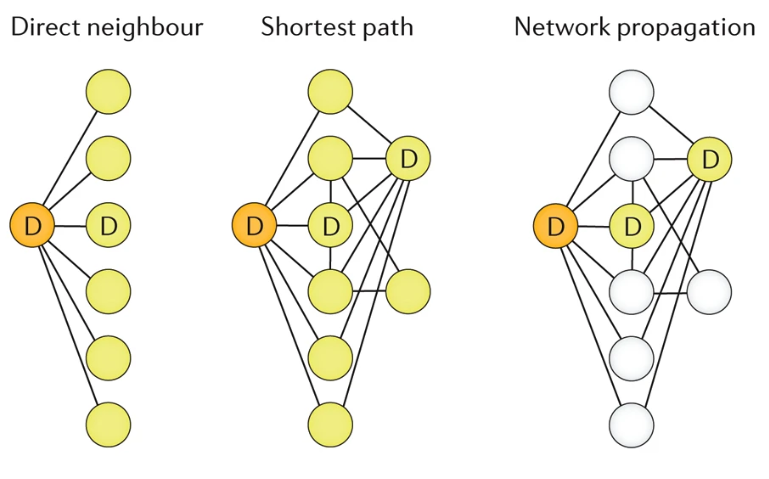
\includegraphics[width=.6\textwidth]{resources/images/Intro/clustering_methods.PNG}
    \caption[Schematic example of neighborhood clustering, shortest path search and network propagation]{\textbf{Schematic example of neighborhood clustering, shortest path search and network propagation. }A single network node (D, orange) with a known function is used to identify other potential functionally related nodes (D, yellow).\\\citep{Cowen.2017}}
    \label{fig:clustering_methods}
\end{figure}
While the two methods described above can yield presentable results for simpler applications they should only be used to quickly analyze more complex data. Predicting relationships and functional interactions in complex biological networks by means of simple mathematical clustering be it scored or not is not feasible due to the high amount of processing that has to be done to the data to decrease the amount of false positives and negatives. \cite{Cowen.2017} showed that \textit{Network Propagation} is a better way to mine data using complex biological networks. Functionally, Network Propagation transforms a list of query proteins into a proteome-wide profile of similarly regulated proteins. In our case this method can be applied to find proteins that have a similar chromatin binding pattern under specific damage conditions. 
\begin{figure}[H]
    \centering
    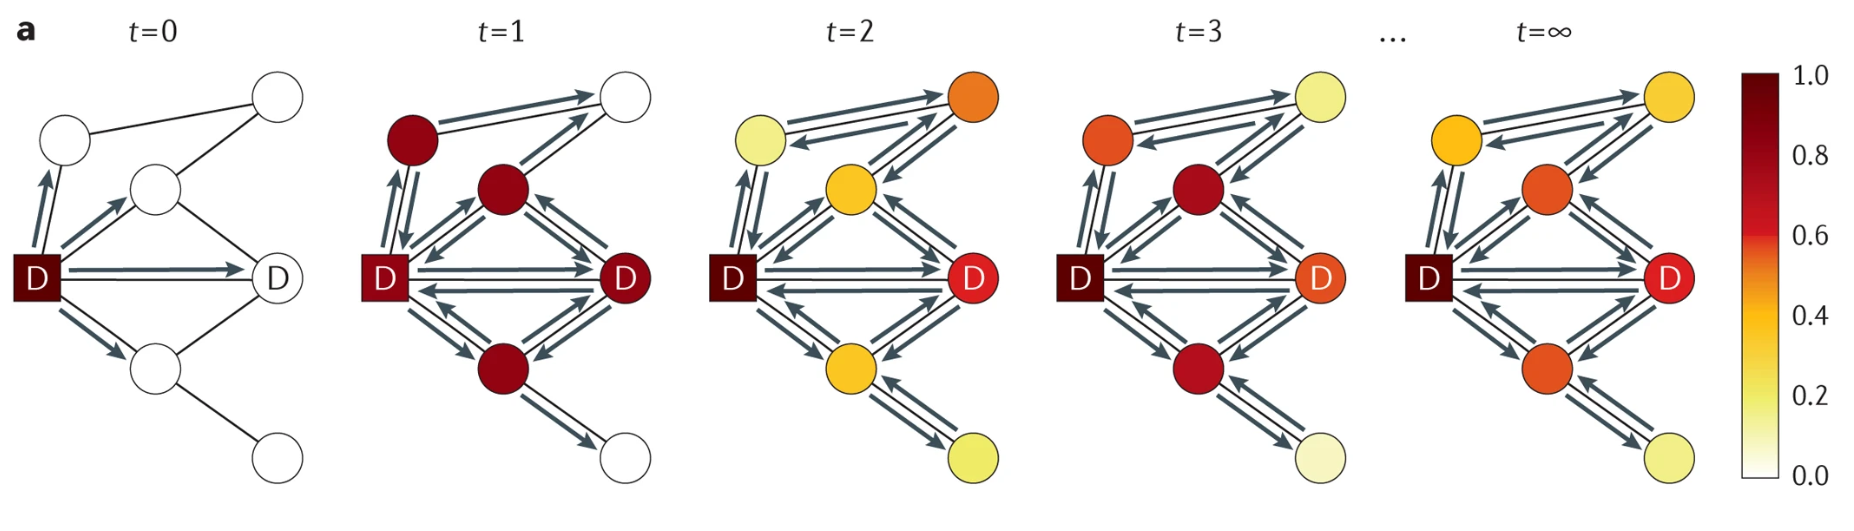
\includegraphics[width=\textwidth]{resources/images/Intro/network_propagation.PNG}
    \caption[Step-by-step demonstration of network propagation]{\textbf{Step-by-step demonstration of network propagation. } Propagation process is shwon at different time points until a steady state is reached ($t=\infty$) and arrows depict the direction of the walk flow. Nodes are colored according to the amount of flow they recieve. D indicates nodes with a known function (square) or with predicted functions (circle).\\\citep{Cowen.2017}}
    \label{fig:network_propagation}
\end{figure}
Network propagation uses a list of proteins with a known function as a query. The have been shown to be capable of identifying previously unknown or predicted disease-associated genes in complex networks ranging from cancer patient data to Alzheimer's research collections \citep{Cowen.2017}. One algorithm belonging to this class is the Google PageRank algorithm \citep{TaherHaveliwala.2003}.
The algorithm gives the query nodes a score of $1.0$ and the score of all other nodes to $0.0$. It then walks along the edges of the network starting at one of the query nodes and at every step each node diffuses its score to its neighboring nodes where the amount it diffuses is proportional to the weight of the edge in weighted networks. This algorithm has been implemented by \cite{Menges.2018} and will be used to mine the DNA Repair Atlas for functional DNA repair modules.
\subsection{Dimensionality Reduction and its applications in High-Throughput Data Analysis}
In addition to analyzing the co-regulation or co-expression of proteins it is often wise to analyze the relationship of the individual experiments that are part of a meta-analysis. For example, a collection of 48 proteomic experiments consisting of about 400 measurements in total with around 5000 proteins identified per measurement can be represented as a matrix with 96,000,000 dimensions. The relationship between the different conditions can teach a data scientist about the integrity of each set and allows , for example, filtering for outliers. In general, dimensionality reduction is used to identify driving components of high-dimensional data sets (i.e. Principle Component Analysis) or to visualize the relationship of individual sets in large collections (i.e. t-Distributed Stochastic Neighbor Embedding) as demonstrated by \cite{Kustatscher.2019}.

\subsubsection{t-Distributed Stochastic Neighbor Embedding}
t-Distributed Stochastic Neighbor Embedding (t-SNE) is a non-linear dimensionality reduction algorithm that has been implemented in different programming languages to be used in multiple data analysis toolkits. It was initially developed as a machine learning algorithm for visualization by L. van der Maaten and G. Hinton \citep{vanderMaaten.2008} that is especially useful for visualising relationships between high-dimensional datasets in a low-dimensional space. t-SNE is comprised of two main steps:\\
A probability distribution over pairs of high-dimensional objects is constructed in such a way that similar objects have a high probability of being selected.\\
After that similar distributions are constructed for a low-dimensional map and the one with the lowest "Kullback-Leibler divergence" with respect to the position of map points to the high-dimensional map is selected. Due to simplicity, the mathematical details of the algorithm are not shown here but can be found in the paper linked above.\\
t-SNE is a useful tool for working with large collections of data because it allows the comparison of individual parts of the collection with one another on a low-dimensional map. This is especially the case if one wants to identify local structures of complex collections i.e. the relationship between different replicates or treatment conditions in one of the included experiment sets while still maintaining information about the global structure of the data collection \cite{Kobak.2019}. In this thesis this algorithm was used to see whether the experiment sets included in the atlas can be compared with one another without loosing information about the individual sets themselves.
\newpage
% Analyse
\section{Results}\label{sec:results}
\begin{center}
    All scripts used in this thesis can be found on my \hyperlink{https://github.com/BaQBone/DNARepairAtlas}{Github} or under github.com/BaQBone/DNARepairAtlas. 
\end{center}
The DNA Repair Atlas (DRA) is an already developed but not yet published web-based resource for the identification of functional DNA repair modules based on quantitative label-free proteomic data collected in the last 12 years. It has been in a constant state of development since then \citep{Menges.2018} and the main goal of this work is to substantially improve its user experience and the feature set. Large parts of this result section are therefore based on optimizations of existing functions  as well as improvements to the usability of the administrator. Direct code and runtime comparisons will be omitted to focus on newly implemented features. Most of the functionality implemented has been reused unless stated otherwise. The data used in the DRA used different DNA lesions, inhibitors and extract systems to study the recruitment of DNA repair factors to chromatin under specific conditions in a time-dependent manner by means of the CHROMASS and PP-MS workflows described above. All of the data used in this thesis were already pre-processed and some subsets focusing on individual DNA repair pathways were already published \citep{Raschle.2015,Haahr.2016}. While combining such a diverse collection of data to form one comprehensive picture is a challenge in itself, the user-experience has to be considered when developing a resource that is supposed to be used by scientists around the world.\\\\
The basic features of the DNA Repair Atlas include the visualization of individual protein raw and normalized abundances over time for each experiment as well as the possibility to check if a protein of interest is significantly enriched in one of the experiments included in the DRA via polar and Volcano plots. The main feature of the DRA are networks that are either heavily pre-filtered and curated to reflect our current understanding of DNA repair or that are mostly unfiltered to allow for the identification of novel interactions of known chromatin-binding proteins under specific DNA lesion conditions using two different clustering algorithms. 
\begin{figure}[H]
    \centering
    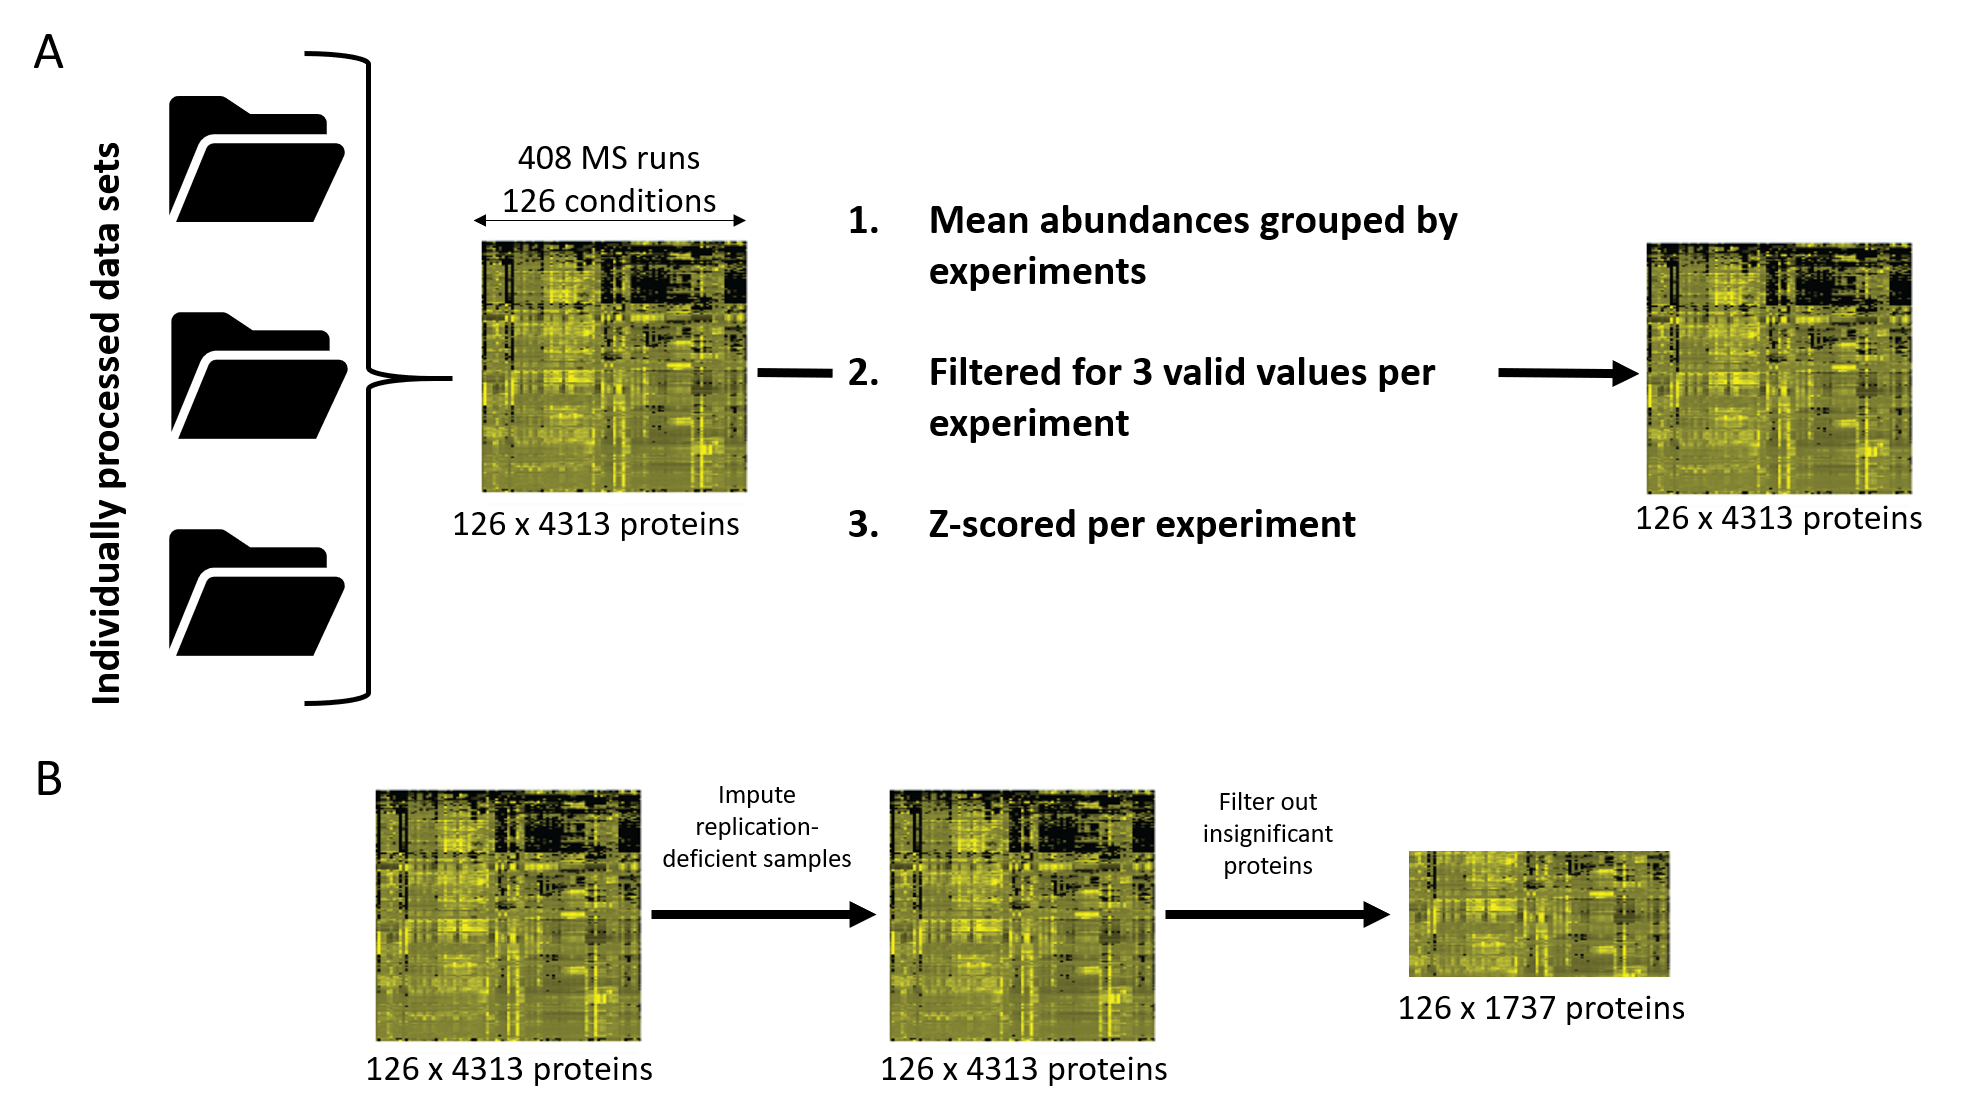
\includegraphics[width=\textwidth]{resources/images/Results/processing_step2.png}
    \caption[Processing of all datasets for visualization.]{\textbf{Processing of all datasets for visualization. }A) All individually processed data sets were combined into one large matrix containing abundances for 4313 proteins over 127 conditions collected in 408 mass spectrometry runs. The mean abundances per replicate where calculated and used to filter each protein for three valid values. This reduced the matrix to 1272 proteins over all conditions that where then Z-scored per experiment to normalize the abundance variation between them. This matrix was used as the input for all further computational methods. B) To improve performance of correlation and clustering algorithms the normalized matrix was further processed. First missing values in replication-deficient data sets were imputed utilizing a pseudo-random bootstrap method by replacing them with values from a normal distribution calculated from the rest of the abundances measured in the experiment. This imputed matrix was then filtered for proteins found to be significantly enriched under the investigated DNA lesions and already known and annotated DNA repair and replication proteins were added afterwards. The resulting matrix of 127 conditions with 1737 proteins each were used to construct new repair networks using Pearson correlation and Topological Overlap Measures.}
    \label{fig:processing}
\end{figure}

\begin{figure}[H]
    \centering
    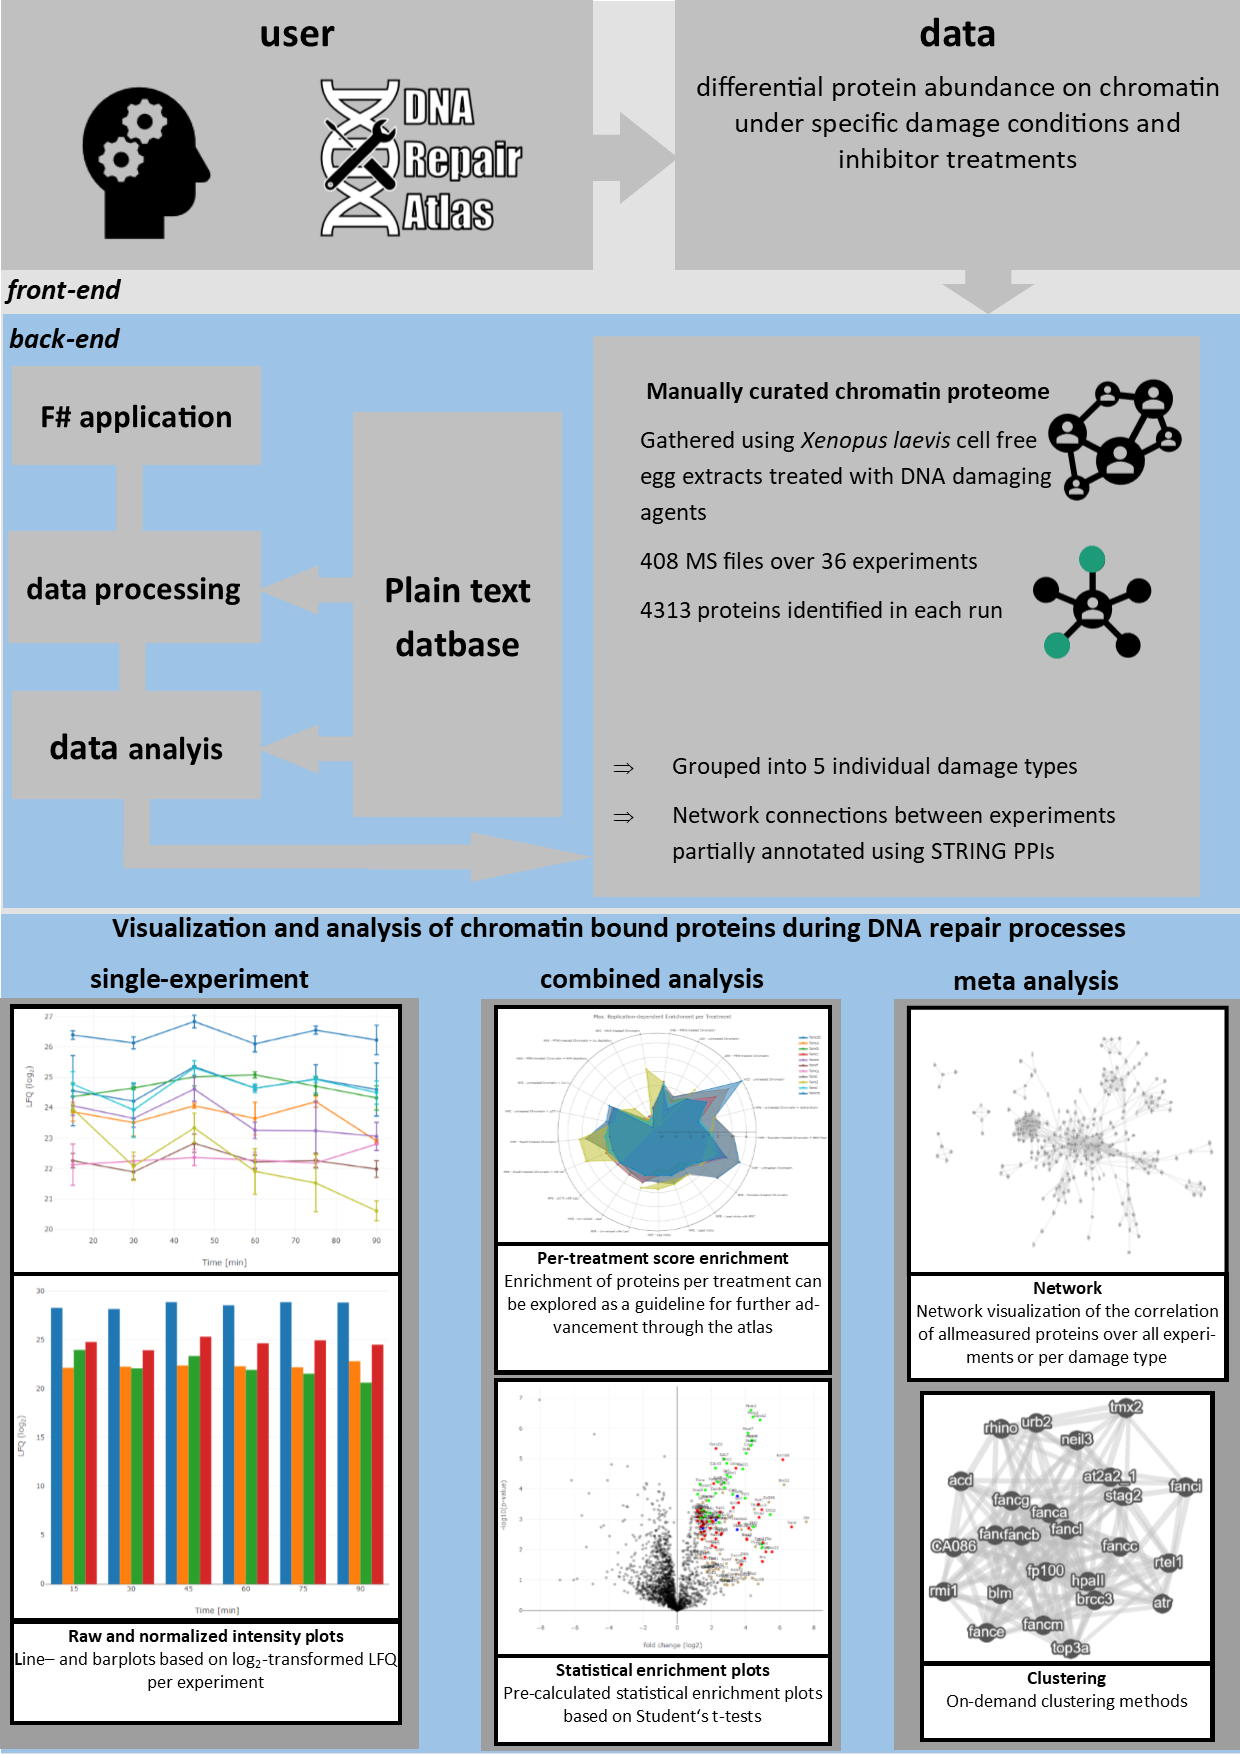
\includegraphics[width=\textwidth]{resources/images/Results/FlowChart.png}
\end{figure}
\newpage
\begin{center}
    \captionof{figure}[Setup and function of the DNA Repair Atlas]{\textbf{Setup and function of the DNA Repair Atlas.} A network representation of protein correlations based on their abundance on chromatin under different damaging conditions represents the central part of the DNA Repair Atlas. The measured \textit{Xenopus} proteins are mapped to the human homologue and annotated with links to protein/gene databases such as UniProt and GeneCard to improve access to the resource for new users. Due to restraints put on the project by the web-deployment method of choice all data needed for the processing and analysis are stored in a plain text database. Data processing and analysis is done on-demand after input from the user using scripts written in the functional programming language F\# running the \textit{back-end} of the resource. The user input as well as the information the \textit{back-end} returns are processed using JavaScript scripts at the \textit{front-end}. Several interfaces are implemented into the DNA Repair Atlas that allow easy access to the five main functions of the resource.}
    \label{fig:flowchart}
\end{center}
The user interacts with an HTML-based front-end deployed on a virtual machine hosted by the RHRK with 1 vCPU, 4 GB RAM and a 60 GB vDisk using Microsoft's Internet Information Service set up as a .NET application web-server. This front-end consists of different subpages with each of them focusing on one category of functions mentioned in Figure \ref{fig:flowchart}. Connecting this front-end to the back-end are scripts written in JavaScript that listen for pre-specified user-interactions and then send the information provided by the user to the back-end which in itself uses the library \textbf{Suave.IO} to listen for a specific set of information.
The back-end consists of a collection of modules written in the functional programming language F\# built mostly by Paul Menges during his master thesis \citep{Menges.2018} that are called using the information received by Suave.IO and return an output based on pre-defined permutations based on the input data. Streamlining and optimizing most of those modules and therefore maximize the user experience was one of this works main goals.\newpage
\subsection{Data (pre-)preprocessing}
\label{sec:processing}
A large part of this project was to optimize the pre-processing of the 408 input data sets based on proteomic analysis of chromatin bound proteins in \textit{Xenopus laevis} egg extracts. Due to the time span over which the data was collected and because it is advised if one wants to combine different collections of data in one large meta analysis we wanted to see how each group of experiments behaves in respect to all others. To do this the non-linear dimensionality reduction algorithm t-SNE was applied to a matrix of mean protein abundances over all time points and replicates of each experiment where columns represented experiments and rows defined protein abundances.\\ t-SNE itself uses the parameters \textit{dims}, \textit{theta} and \textit{perplexity} to alter the location of each data point on the map. \textit{Dims} can either be set to $2$ or $3$ and defines the dimensions one wants to reduce the high-dimensional data set to. In most biological circumstances two dimensions are sufficient to visualize relationships between data points. \textit{Theta} should always be set to $0.0$ for best results as it defines the error between different iterations the algorithm deems to be sufficient. Higher \textit{theta}-values improve computation times with a decrease in accuracy. The parameter \textit{perplexity} (loosely) defines how to balance  attention between local and global aspects of the input data and sort of "guesses" the number of close neighbours of each data point on the map. Due to this it always has to be smaller than the number of data points one wants to look at.\\
\begin{figure}[H]
    \centering
    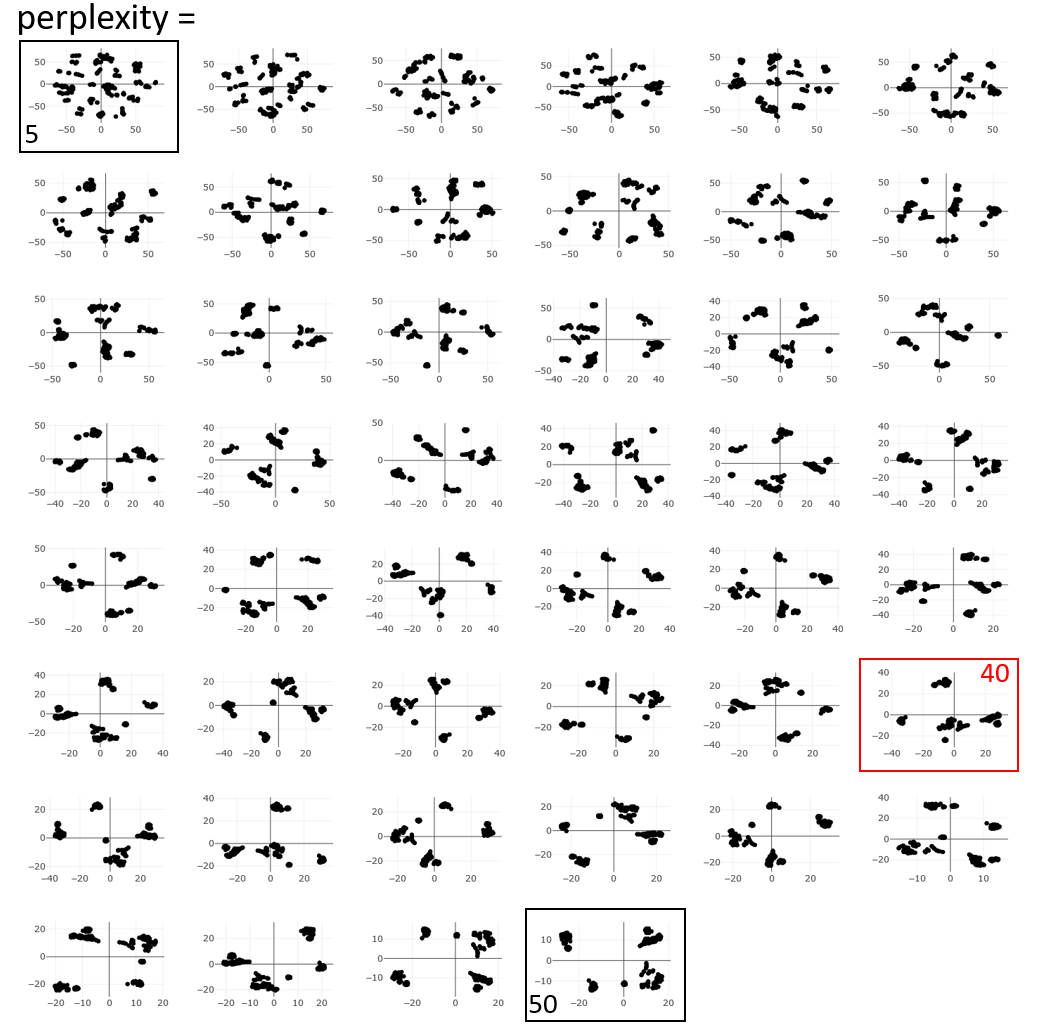
\includegraphics[width=\textwidth]{resources/images/Results/tSNE_opti.png}
    \caption[t-SNE Perplexity Optimization]{\textbf{t-SNE Perplexity Optimization. } A non-normalized matrix of mean protein abundances per experiment was filtered to include only the 1000 most prominent proteins based on their known ability to bind chromatin to lower computation times. \textit{theta} was set to 0.0 while \textit{perplexity} iterated from 5 to 50 in increments of 1. After comparing all resulting t-SNE maps we decided to continue with $perplexity = 40$ to avoid large indistinguishable groups.}
    \label{fig:tsneopti}
\end{figure}
To optimize the \textit{perplexity} for our use case we made the assumption that the result should show our data in two main and seven sub-groups that each represent the two different DNA templates, sperm chromatin and plasmid DNA, and the six different induced damages for each set of experiments. After applying t-SNE with perplexities between 5 and 50 to a pre-filtered data set we decided on \textit{dim} $= 2$, \textit{perplexity} $= 40$ and \textit{theta} $= 0.0$ for the final large scale t-SNE.\\
Those parameters resulted in the final map of all experiments shown below.
\begin{figure}[H]
    \centering
    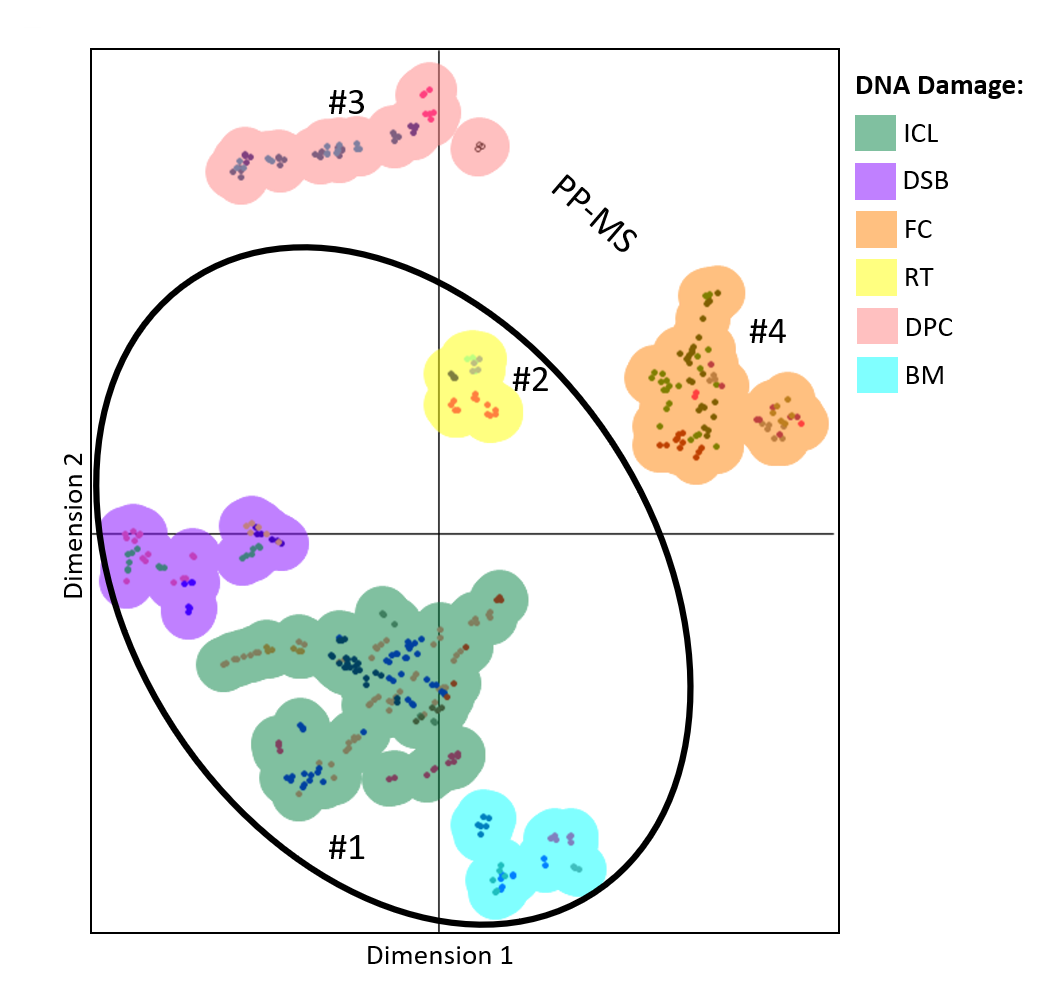
\includegraphics[width=.6\textwidth]{resources/images/Results/tSNE_map.png}
    \caption[Two-dimensional t-SNE map of all sets included in the Atlas]{\textbf{Two-dimensional t-SNE map of all sets included in the Atlas. }Non-normalized mean protein abundances for each experiment were used as an input for the t-SNE using the optimized parameters mentioned above. Colored clouds represent DNA lesions with: ICL = Interstrand Crosslink, DSB = Double-Strand Break, FC = Replication Fork Collapse, RT = Replication Termination, DPC = DNA-Protein Crosslink, BM = Base misincorporation. Data points included in the black ellipse represent experiment using sperm chromatin as the DNA while the others use plasmid vectors with defined lesions. Individual points inside the clouds each represent a single experiment and time point while their colors encode their chemical treatment (not of importance for this section). Numbers next to each group indicate the batch the sets were processed in due to their use in different publications.}
    \label{fig:tsnemap}
\end{figure}
Figure \ref{fig:tsnemap} shows a close relationship between all sets using sperm chromatin as a template (black ellipse) while still retaining closer grouping between each experiment series and the damage type induced respectively (cloud colors). Inside the larger clouds that represent experiment series each data point is individually colored in respect to its treatment. For example point colored pink always represent experiments using Geminin-treated extracts. Looking especially at the experiments colored in pink that are all deficient in DNA replication one can see them grouping away from replicating extracts of the same series while remaining in close vicinity.\\
As already mentioned some of the experiment sets were processed together in one processing session based on the publication they were used in (on the map indicated by \#1 through \#4). We previously expected this circumstance to have a large impact on the neighborhood on the t-SNE map but this does not seem to be the case. Neighborhood embedding seems to strongly depend on the DNA template and extract type used as well as the precise stage of replication and repair the experiment was focusing on. We can see this especially for processing group \#2 that uses sperm chromatin as a template but does not seem to embed closely to other experiments using the same substrate. This can be explained due to the experiment setup in general that was focused on investigating the termination of DNA replication specifically.  Due to the specific protein fingerprint of replication termination in comparison to all other sets and the synchronous nature of these experiments this group of experiments embeds distant from the other CHROMASS data sets and closer to the PP-MS sets were replication is more synchronized compared to CHROMASS. The PP-MS sets also embed far away from each other as expected due to the synchronized replication and the very strictly defined lesions present on the plasmid template.\\
From this preliminary data investigation using dimensionality reduction to build a neighborhood map of all experiments included in the atlas we can conclude that DNA template and lesions have a higher impact on the embedding of each experiment series. While still present, the effect of batch processing can be neglected once proper normalization steps are carried out for the whole collection of data sets. This is proves that the previous approach to visualizing DNA repair modules using a normalized pre-filtered network on the atlas was valid but could be improved by adding networks for each type of DNA lesion. Implementing such networks can, as will be discussed later in this thesis, noticeably improve the performance of clustering algorithms for the identification of functional DNA repair modules. t-SNE analysis showed that the sets are usable for the purposes of the DNA Repair Atlas but could be reprocessed together once the computational resources are available.\\
After validating that the data can be combined without batch effects inhibiting the creation of repair networks we moved on to prepare the data sets.\\\\
To enable filtering of significantly enriched proteins in later steps we used the combined matrix of protein abundances as an input for an R script utilizing Student's t-Tests with data dependent S\textsubscript{0} determination. This script used the package "samr" (https://CRAN.R-project.org/package=samr) to determine the S\textsubscript{0} for each comparison dependent on the data itself. This allowed us to automate the calculation of significance values for each protein regarding its enrichment based on predefined comparisons. The resulting p-values were stored in log\textsubscript{10} format and afterwards multiplied over all comparisons to obtain an arbitrary "Enrichment Score" over all experiments as well as for each DNA lesion separately. This score is used in the DRA in network styling as well as the base for the polar enrichment plot of each DNA lesion.\\  
As briefly described in Fig \ref{fig:processing} the individual data collections were combined into one matrix consisting of all 408 mass spectrometry runs over 126 conditions. In each run, a total of 4313 proteins could be detected whose mean abundances per replicate were calculated. For each experiment proteins with less than three valid values were filtered out.  This yielded a matrix with 1727 proteins over 126 conditions retaining time point information that was used as an input for the visualization functions of raw and normalized abundances for each experiment. As will later be shown the functions enabling this feature have been optimized to be more modular and user friendly.\\\\
To build the aforementioned networks for each type of DNA lesion this matrix was further processed to only include one value per protein for each experimental condition. Those conditions then were grouped by the DNA lesion repair they were used to investigate and split into separate matrices while keeping one ungrouped matrix containing all conditions. The "Enrichment Score" over all DNA lesions was filtered for all proteins with a higher score than the 90\textsuperscript{th} percentile to reduce the number of proteins to 1737. This list of proteins was deemed "interesting" and used to filter the individual DNA lesion matrices before applying WGCNA.\\


\subsection{Optimizing an interactive web application}
\label{sec:resource}
The development of an interactive web-resource based on mass spectrometry data is a complex endeavour that ideally starts with a concrete plan of action. This plan has to include the programming language of choice, the basic structure of the final website as well as the so called "handler" that connects back-end and front-end with each other. Additionally it has to be thought about how data is stored and whether or not the user has direct or indirect access to raw or pre-processed data. In our case we decided to build the back-end using the functional programming language \textbf{F\#} developed by Microsoft as part of their .NET Framework using the library \textbf{Suave.IO} to functionally create a webserver with an included link handler. The user front-end (from here on referenced as "website") was written and styled using the markup language HTML (\textit{Hyper Text Markup Language}) and the style sheet language CSS (\textit{Cascading Style Sheet}) in combination with the web-programming language JavaScript as a means to implement local program functionality on the website itself. JavaScript was chosen over alternatives such as the scripting language PHP (originally: \textit{Personal Home Page}; Now: \textit{Hypertext Preprocessor}) due to performance limitations of the hardware used to deploy the resource to the user. With JavaScript, everything except direct request to the back-end runs locally on the users machine where PHP is evaluated by the server itself. Details about this including parts of the code are included in subsection \ref{sec:resource}.\\

The general structure of the resource can be seen in Figure \ref{fig:flowchart}. This flowchart shows the setup of the DNA Repair Atlas as well as the methods used to store data and an overview of the functions provided to the user to explore said data. The core functionalities were only adapted to challenges that arose during a test phase of the DRA and new methods were applied where necessary.\\

The first addition was a feature we call "Protein Search" with which the user can send a list of proteins of interest to the server and the server compares it to a list of registered proteins. If the proteins or any synonyms are found in the plain text database the server returns a list of enrichment scores which are plotted as polar plots using Plotly.js. The scores plotted are based on the filtered enrichment score matrix that only contains the 1737 most significantly enriched proteins over all datasets. The DRA itself offers the possibility to mine data for all 4313 proteins detected in the raw matrix with other features that will be explained later.
\lstset{language=FSharp}
\begin{lstlisting}
let rec radialData 
    (metaData:(string*float*float*float*float*float*float)list) (poi:string*string) =
        match metaData with
        | [] -> []
        | ((prot,all,dpc,dsb,fc,icl,rt) :: rest) when prot = (fst poi) ->
          (prot,dpc,dsb,fc,icl,rt) :: radialData rest poi
        | (_ :: rest) -> radialData rest poi
\end{lstlisting}
This function is especially useful for new users of the atlas that are are interested in the list of proteins included in it. Additionally it is useful to check if a protein one is interested in is significantly enriched in one of the DNA lesion sets included in the DRA. If one is for example interested in the enrichment of the Fanconi anemia core Complex it is possible to plot all subunits at once.
\begin{figure}[H]
    \centering
    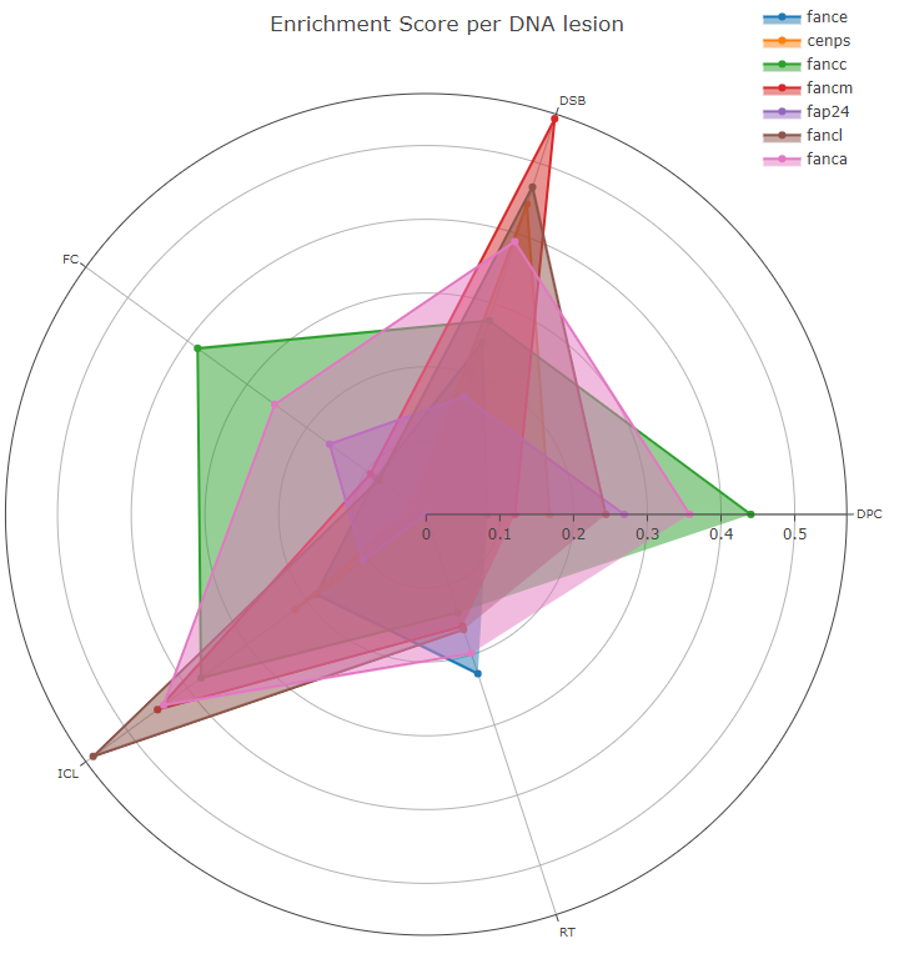
\includegraphics[width=0.6\textwidth]{resources/images/Results/fanc_enrichment.png}
    \caption[Relative enrichment of Fanconi Core Complex subunits]{\textbf{Relative enrichment of Fanconi Core Complex subunits. }Enrichment scores for each subunit of the Fanconi Core Complex included in the filtered list of enriched factors. Included are only those subunits that are enriched over all data sets but the scores are specific to each DNA lesion.}
    \label{fig:fanc_enrichment}
\end{figure}
The figure shows that subunits of the Fanconi Core complex seem to be enriched on chromatin in experiments investigating Interstrand Crosslinks and Doublestrand Breaks but fancc and fanca seem to be slightly enriched in DNA-Protein Crosslink and Replication Termination experiments. This could be an indication of homologueous recombination dependent DPC repair being mediated by the Fanconi anemia pathway in higher eukaryotes \citep{Stingele.2015}. Generally this feature of the DNA Repair Atlas gives the user a good idea of what to expect from the Atlas itself. It provides an overview of which DNA repair pathways can be investigated and how well certain parts of the proteome are represented.
\newpage

The next more detailed part of the DRA is a feature that lets the user plot intensity data over time for each experiment and all 4313 proteins either in LFQ or in normalized LFQ (z-scored) values.\\
Previously, this module was built to only work with the specific plain text database where rows represented individual proteins and each column represented a single proteomic data file. The function written to extract data from this set based on the user input consisting of an experiment is shown below.
\lstset{language=FSharp}
\begin{lstlisting}
let chooseExperiment (exp:string) =
    match exp with //matches the input experiments with pre-defined keys in the database
    |"Key" -> let Exp_Time_1 = 
                    [for row in textDataBase.Rows -> row.Exp_Time_1]
                    |> Seq.ofList 
                    |> Seq.zip miscData
    //and uses FSharp.Data to extract matching intensities per timepoint
              let Exp_Time_2 = 
                    [for row in textDataBase.Rows -> row.Exp_Time_2] 
                    |> Seq.ofList 
                    |> Seq.zip miscData
    //to finally merge to a sequence of two tupled lists containing intensities and time
             seq[Exp_Time_1;Exp_Time_2],["1";"2"]
                   
    |"" -> seq[],[]
\end{lstlisting}
Put simply, this function matches the experiment chosen by the user with \textit{hard coded} experiments in the database, extracts every row of the column representing this experiment and then merges it with a list of proteins defined elsewhere. In the context of the resource this function is called within another function that gets the experiment and a list of proteins of interest as an input and that outputs data in the format the front-end needs to plot a time course or protein intensities for the selected experiment and treatment. To improve on this function design we looked at the input file and how data is extracted from it. Noticeable was that each time a new data set was added to the collection there were two locations in the code that had to be adapted to fit the new input structure. Not only had the HTML document to be updated but also the matching function in the back-end. We came to the conclusion that it would be easier to store the data in such a way that new data sets could be added without the need to update most of the code. To achieve this we implemented a function that takes a plain text file, an experiment, a treatment condition and a list of proteins as its input. The list of proteins is fed to the function in string format to simplify the interaction between the back- and front-end.
\newpage

\lstset{language=FSharp}
\begin{lstlisting}
let searchForProteinData (data:CsvFile<CsvRow>) (expIn:string) (protList:string) (treatIn:string) =
    let lfqValueSeq = 
        let proteins = data.Headers.Value |> Array.tail |> Seq.ofArray
        seq[for i in (addedNames protList) -> proteins |> Seq.filter (fun x -> x.StartsWith(fst i))]
        |> Seq.concat
        |> Seq.map (fun p -> proteins 
                             |> (fun _ -> data.Rows 
                                          |> Seq.map (fun y -> try float (y.GetColumn p) with | :? Collections.Generic.KeyNotFoundException -> nan))
                             |> Seq.zip [for row in data.Rows ->
                                            int (row.GetColumn "FILE_ID")],p)             
    let filteredMeta = 
        let filtered = (metaDataParse.Filter (fun x -> String.Equals((x.GetColumn "Treatment"), treatIn) )).Filter ( fun x -> String.Equals((x.GetColumn "Experiment Series"), expIn))
        seq[for row in filtered.Rows ->
                int (row.GetColumn "FILE_ID"), row.GetColumn "Treatment", row.GetColumn "Experiment Series", row.GetColumn "Time"]
    let treatment = filteredMeta |> Seq.map (fun (_,treat,_,_) -> treat) |> Seq.head
    let inter = 
        filteredMeta 
        |> Seq.collect (fun (metaID,_,_,time) -> (lfqValueSeq |> Seq.map (fun (valueSeq,protName) -> (valueSeq |> Seq.tryFind ( fun (lfqID,_) -> lfqID = metaID),protName,time))))
        |> Seq.map (fun (valOpt,protName,time) -> match valOpt with
                                                  | Some x -> (snd x), protName,time
                                                  | None -> nan,protName,time)
    inter
    |> Seq.filter (fun (lfq,_,_) -> (Double.IsNaN >> not) lfq )                      
    |> Seq.groupBy (fun (_,y,z) -> y,z) 
    |> Seq.map (fun (groupName,myGroup) -> groupName,(myGroup |> Seq.map ( fun (lfq,_,time) -> lfq,time)))   
    |> Seq.map (fun ((p,t),x) -> (p,t),(List.ofSeq x |> List.unzip))
    |> Seq.map (fun ((p,t),(vL,_)) -> p,vL,t,(List.averageBy float vL),(sDev vL))
    |> Seq.groupBy (fun (p,_,_,_,_) -> p)
    |> Seq.map (fun (groups,data) -> groups,data |> Seq.map ( fun (_,_,t,vm,e) -> (vm,e,t) ) |> List.ofSeq |> List.unzip3)
    |> Seq.map (fun (n,(y,e,x)) -> (n,treatment,(y,e,x)))
    |> Seq.sortByDescending (fun (prot,_,(_,_,_)) -> prot)
\end{lstlisting}
Note that in this case the data is split into two files with one containing meta information and the other the LFQ intensities. The two files are matched using unique IDs. This format was chosen to make it easier to maintain the meta data and make changes on the fly without risking to alter the LFQ intensity file. In general applying this function results in the same output as the function mentioned above, but the mechanism by which it works allows easier maintenance.\\
Additionally this change gave way to a dynamically filled drop-down menu on the front-end. Each time an experiment series is selected (see Figure \ref{fig:dropdown_plotting}) the drop-down menu for selecting the experimental condition is updated to show all valid options. To do this the front-end request a JSON string containing a map of experiment series and their valid conditions anytime the experiment selector is changed. 
\begin{figure}[H]
    \centering
    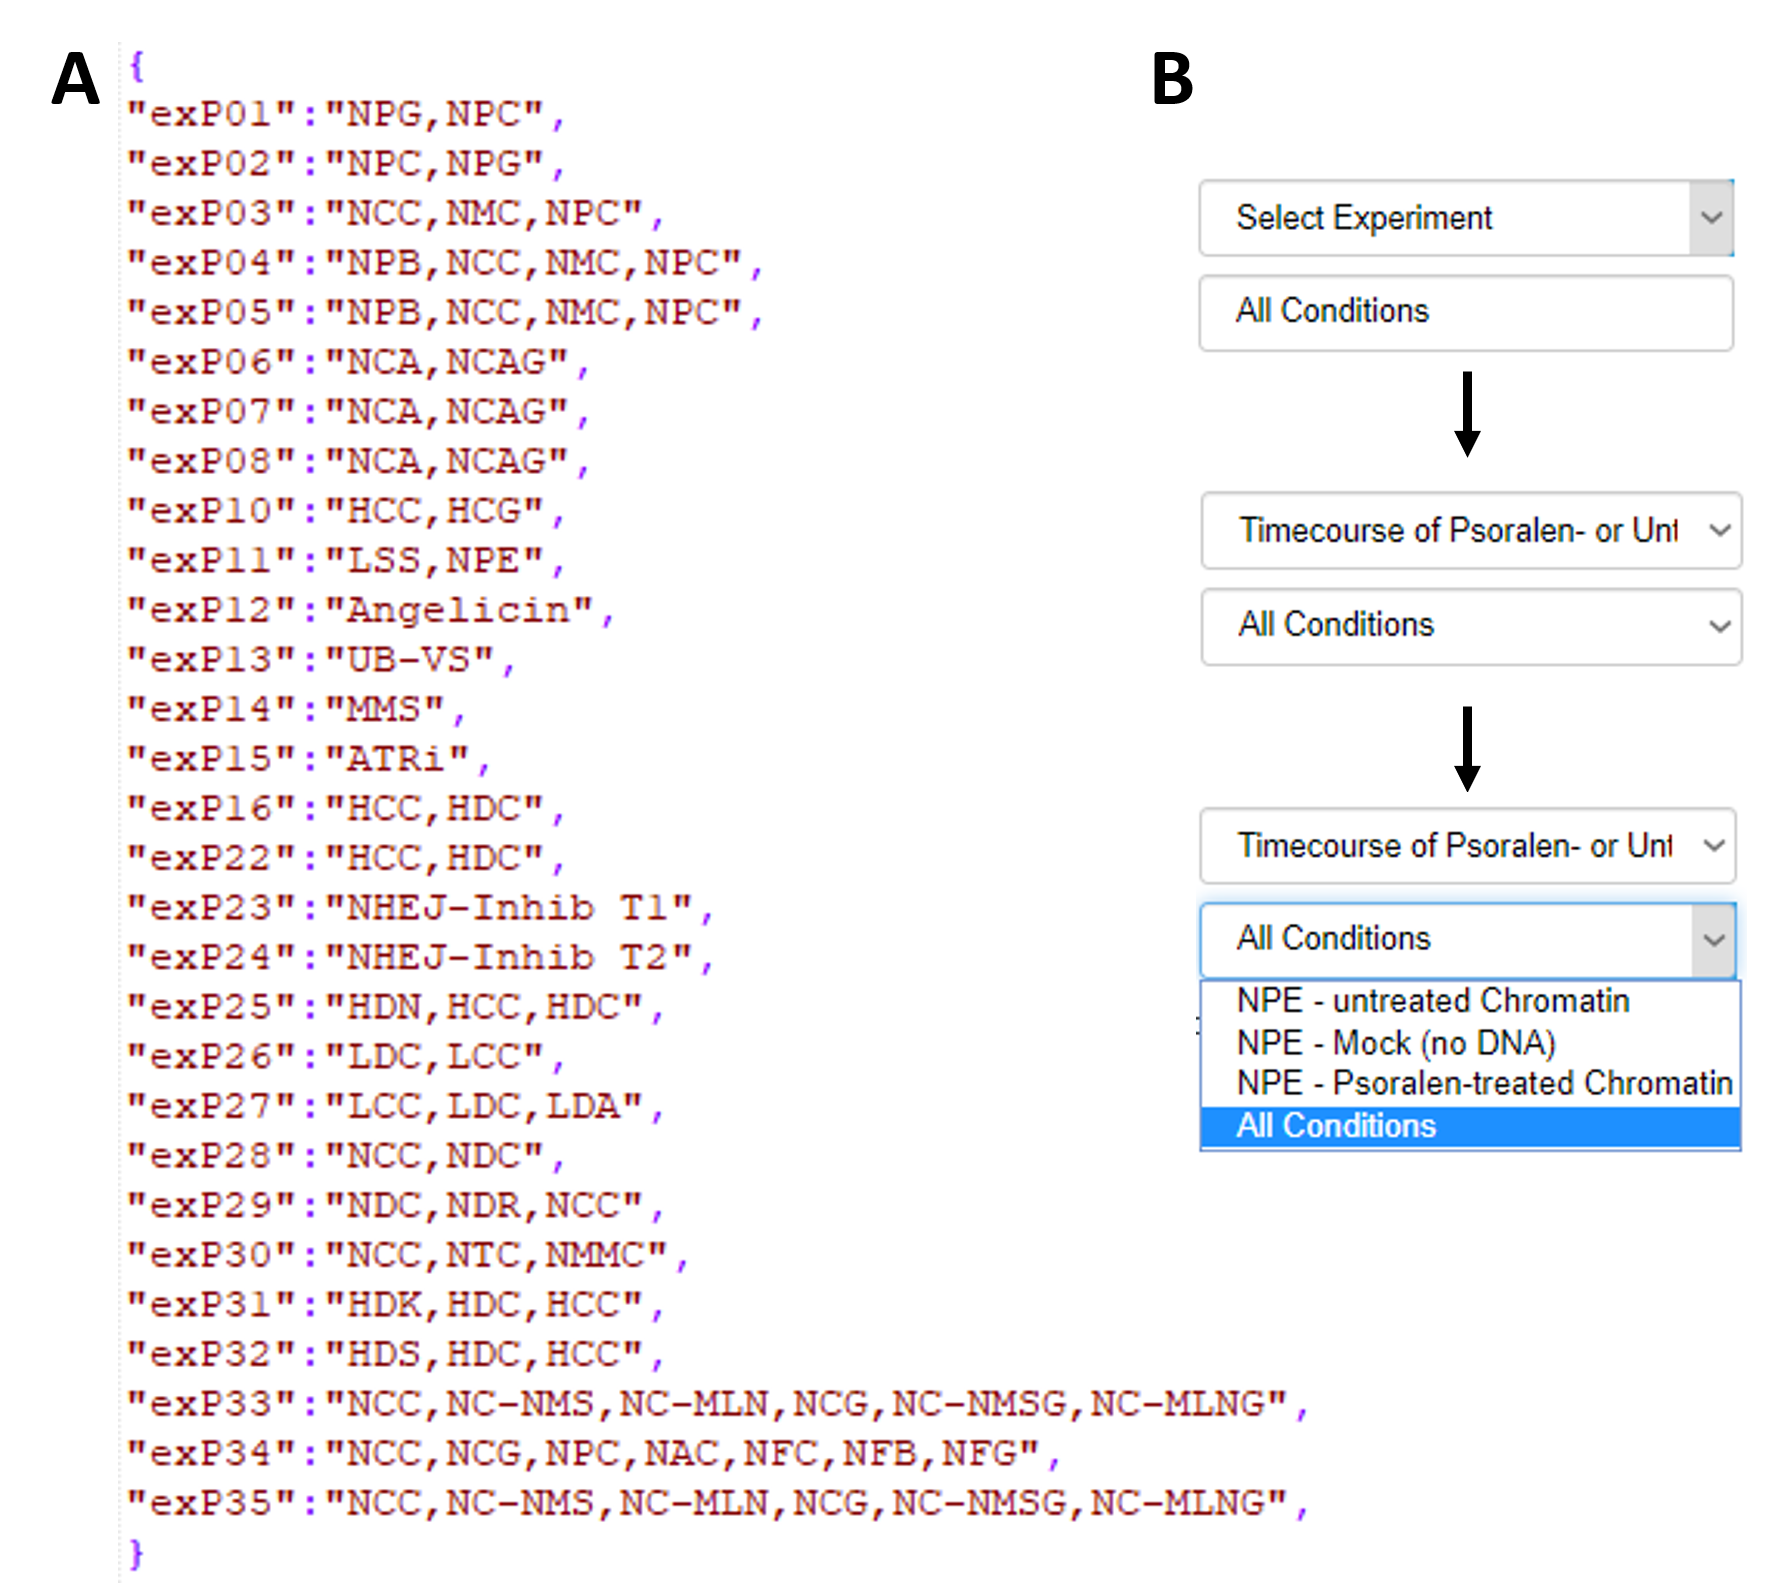
\includegraphics[width=.7\textwidth]{resources/images/Results/dropdown_plotting.png}
    \caption[Filling a Drop-Down menu with JSON data]{\textbf{Filling a Drop-Down menu with JSON data. }A) Illsutarted is the JSON string the front-end request each time the experiment selector is changed. The JSON string represents a map that contains keys representing individual experiments that are matched via a JavaScript function and respective values that are used to fill the second dropdown menu dynamically. B) An overview of the drop-down menus used to select an experiment and the dynamically filled treatment.}
    \label{fig:dropdown_plotting}
\end{figure}
The dynamic addition and removal of drop-down options given the described JSON map is handled via the following JavaScript function. This function uses a switch-case statement to match key values of the JSON map requested from the back-end to extract their respective values. It then uses another switch-case statement to match the three-letter treatment codes with human readable treatment descriptions that are added to the treatment selection drop-down menu.\\
\newpage
\lstset{language=htmlcssjs}
\begin{lstlisting}
function updateTreatments() {
    var $dropdown = $("#exp");
    $.getJSON("/expList", function (expdata) {
        var key = $dropdown.val();
        var vals = [];
        //matches JSON string keys with current experiment drop-down value and returns corresponding treatment codes
        switch (key) {
            case 'EXP01':
                vals = expdata.exP01.split(',');
                break;
            case 'EXP02':
                vals = expdata.exP02.split(',');
                break;
            case 'EXP03':
                vals = expdata.exP03.split(',');
                break;
            ...
            case 'base':
                vals = ['<option>Can not switch to</option>'];
        }
        //matches the extracted treament codes from the JSON string and returns drop-down items
        var $treatChoice = $("#treat");
        $treatChoice.empty();
        $.each(vals, function (index, value) {
            switch (value) {
                case 'NCC':
                    $treatChoice.append('<option value = "' + value + '">NPE - untreated Chromatin</option>');
                    break;
                case 'NMC':
                    $treatChoice.append('<option value = "' + value + '">NPE - Mock (no DNA)</option>');
                    break;
                case 'NPC':
                    $treatChoice.append('<option value = "' + value + '">NPE - Psoralen-treated Chromatin</option>');
                    break;
                case 'NPG':
                    $treatChoice.append('<option value = "' + value + '">NPE - Psoralen-treated Chromatin + Geminin</option>');
                    break;
                ...
                default:
                    $treatChoice.append('<option value = "' + value + '">' + value + '</option>');
                    break;
            }
        });
        $treatChoice.append('<option value ="' + vals + '" selected>All Conditions</option>');
    });
}; 
\end{lstlisting}
The last version of the DRA included only the option to use specific predefined protein names as an input for the plotting- and search functions. This has been updated to include the UniProtIDs for each human homologue of the included proteins as well as major Gene Ontology (GO) codes (Cellular Compartment = CC; Biological Process = BP; Molecular Function = MF). This gives the user the opportunity to input a certain GO-term and plot all proteins in the database that are annotated with that term. For example if a user is interested in the changes of protein abundance on Psoralen-treated chromatin over time for the Fanconi anemia complex proteins it is not necessary to type each subunit into the input field but the GO term would be sufficient.
\begin{figure}[H]
    \centering
    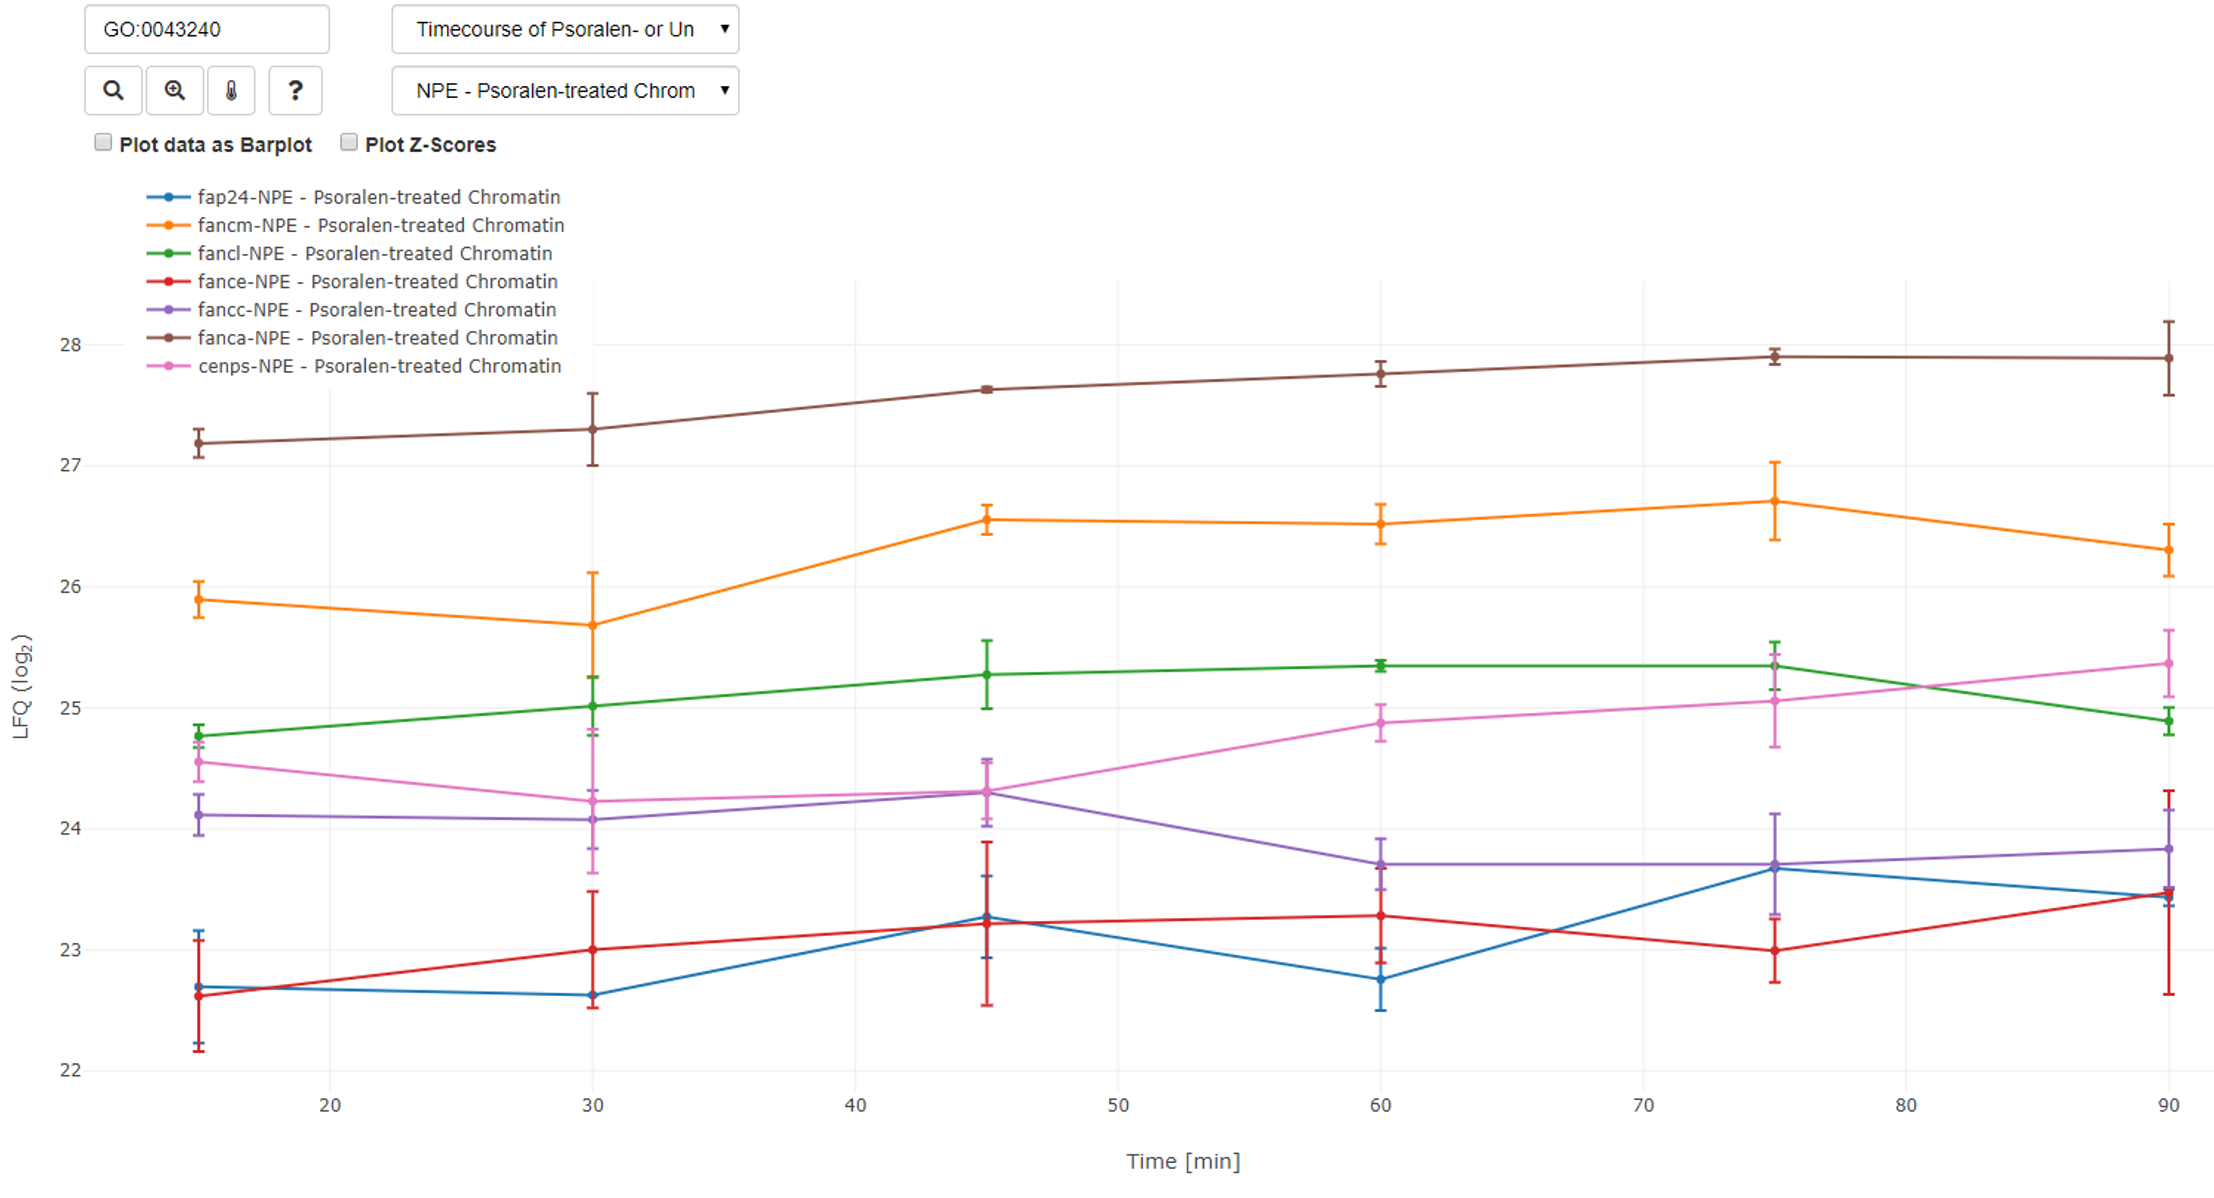
\includegraphics[width=\textwidth]{resources/images/Results/fanc_plottingPso.png}
    \caption[Supplementary Intensity Plots]{\textbf{Supplementary Intensity Plots. }The DRA features the option to plot the changes in abundance on chromatin for each included protein, experiment and experimental condition. The user has the option to either plot line- or bar plots over time given the standard deviation as error bars per time point as well as normalized (z-scored) intensities without error bars.}
    \label{fig:fanc_plotting}
\end{figure}
This feature has been implemented globally so that it functions with all basic input fields on the DRA. Functionally the back-end stores all annotation data for each protein in a large plain text table with the structure shown in Figure \ref{fig:annotation} and applies a function called \textit{addedNames} to every text input made by the user.
\newpage
\begin{wrapfigure}{l}{0.4\textwidth}
    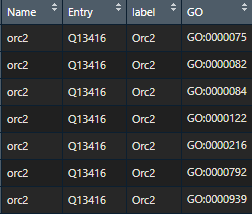
\includegraphics[width=0.36\textwidth]{resources/images/Results/annotation.PNG}
    \caption[Small excerpt from the annotation table used for data mining]{\textbf{Small excerpt from the annotation table used for data mining. }Shown is a list of additional names for the Origin Recognition Complex subunit orc2. Note that each row represents a single given combination of all possible inputs that result in orc2 being used as a query protein. Available are a multitude of GO terms (GO) as well as the gene name (Name), an alternative gene name (label), human homologue UniProtID (Entry).}
    \label{fig:annotation}
\end{wrapfigure}
\textit{addedNames} takes the user input string which can be a single protein of interest, a list of proteins or a GO term and splits it into a Sequence of strings. Each element of this sequence is then matched against a protein annotation file containing multiple entries for each protein present in the database based on ever single possible GO term and UniProtID for that protein. If a match is found, the function returns a list of proteins with identification values that match the ones used in the plain text data base of the DRA, effectively translating known alternative names and IDs to usable protein names. As this function can be called inside any other function extracting information for a protein from the data base, we've implemented a way to use multiple identification systems with the DRA that can be easily adapted once new proteins get added or more identifiers are needed. Especially useful is the inclusion of GO terms due to their ease of use and the possibility to use them as an easier input for clustering algorithms using multiple proteins as their input - such as the Diffusion algorithm implemented in the DRA by \cite{Menges.2018} (see Section \ref{sec:diffusion}).
\lstset{language=FSharp}
\begin{lstlisting}
let addedNames (inString:string) =
    inString.Split [|',';';'|] |> Array.filter (String.IsNullOrWhiteSpace >> not) |> Array.map ( fun x -> x.Trim()) |> Seq.ofArray
    |> Seq.collect ( fun inputProt -> 
                     additionalNames 
                     |> List.map ( fun x -> 
                                   match x with
                                   | (a,_,_,_) when String.Equals (a,inputProt) -> a,inputProt 
                                   | (a,b,_,_) when String.Equals (b,inputProt) -> a,inputProt 
                                   | (a,_,c,_) when String.Equals (c,inputProt) -> a,inputProt
                                   | (a,_,_,d) when String.Equals (d,inputProt) -> a,inputProt
                                   | _ -> inputProt,inputProt ) )
    |> Seq.distinctBy fst
    |> ( fun x -> if (inString.StartsWith "GO:") || (inString.StartsWith "EC:") then
                    x |> Seq.filter ( fun (a,b) -> not (String.Equals (a,b)) )
                  else
                    x)
    |> Seq.filter ( fun (a,b) -> (String.IsNullOrWhiteSpace >> not) a )
    |> List.ofSeq
\end{lstlisting}\newpage
\begin{figure}[H]
    \centering
    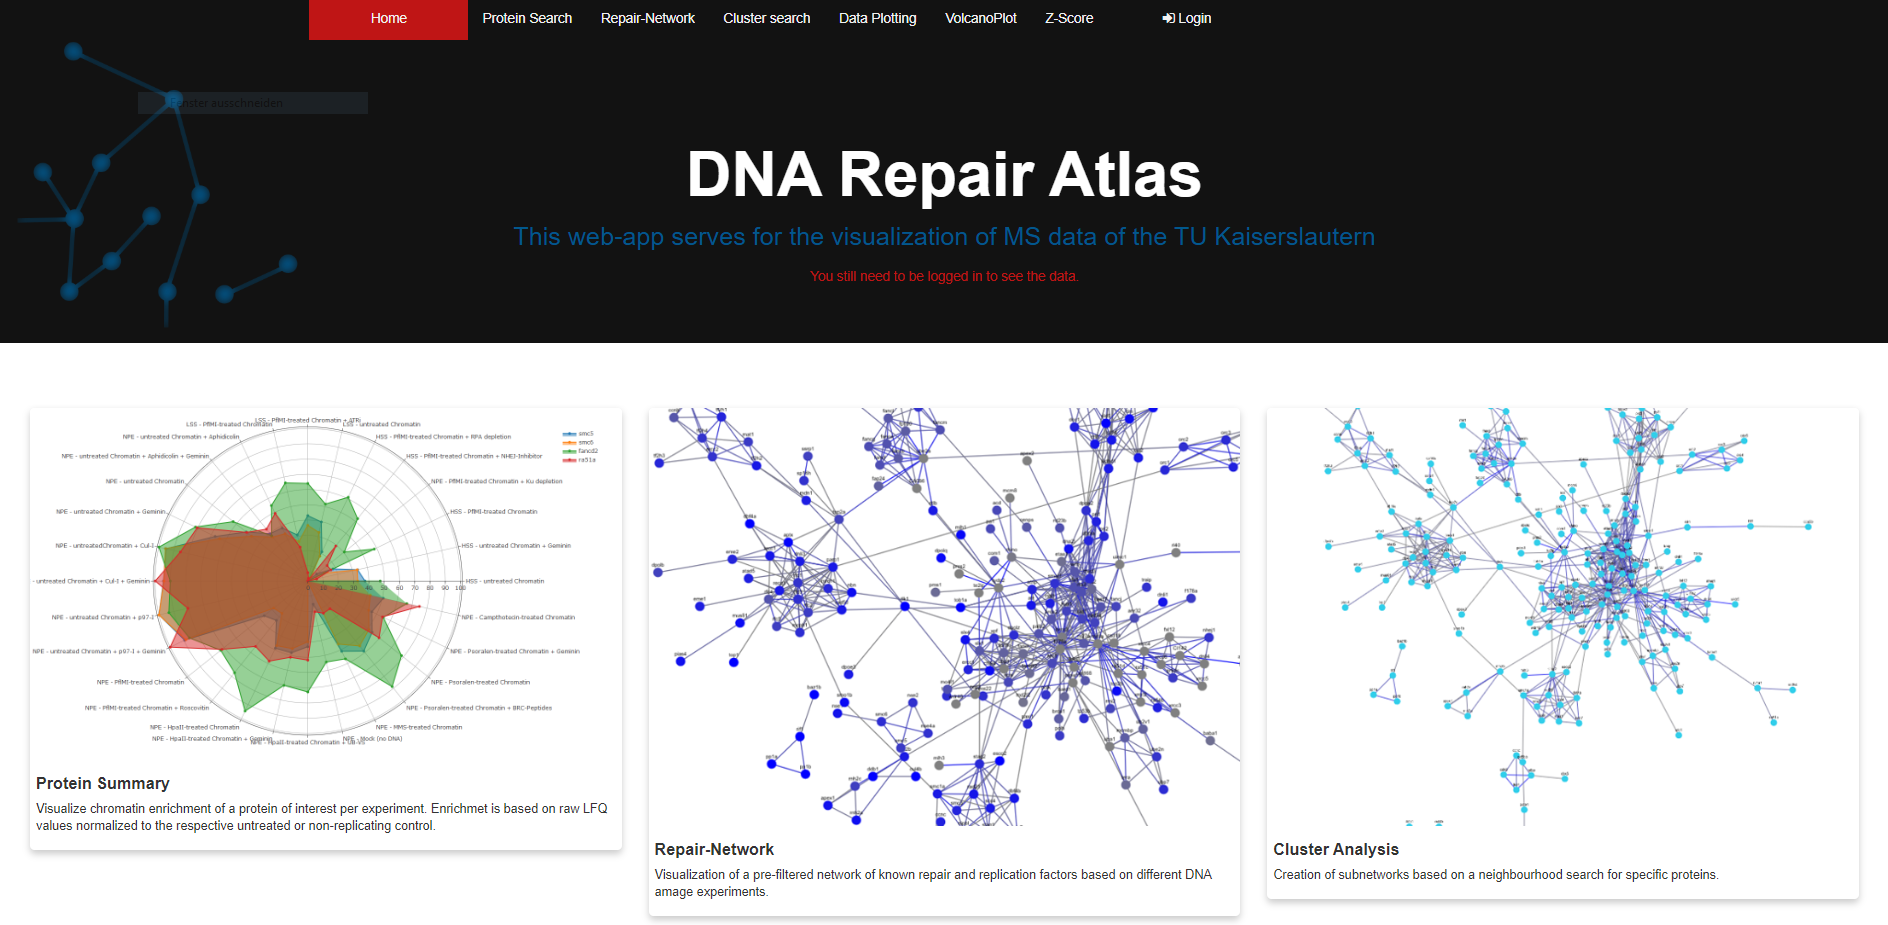
\includegraphics[width=\textwidth]{resources/images/Results/home.PNG}
    \caption[Screenshot of the starting page of the DNA Repair Atlas]{\textbf{Screenshot of the starting page of the DNA Repair Atlas. }Shown is a screenshot of the starting page with the visual represenations of all major functions as well as descriptive texts for each of the sub-pages.}
    \label{fig:home}
\end{figure}
In addition to some changes on a functional level the design of the DRA has been updated to improve the user experience. The starting page now shows a visual representation of all included functionalities as well as descriptive texts for each major sub-page.\\
For the remainder of this thesis we will focus on the \textbf{Cluster Search} starting with how the networks that can be plotted were created and what they can be used for.

\subsubsection{Constructing DNA lesion specific networks using modified WGCNA}
\label{sec:netprocessing}
Filtered matrices for each DNA lesion were transposed so that columns represented proteins. Due to the low number of experiment sets included in the collection for Base Misincorporations we omitted this set from the network creation. The Pearson correlation coefficient for each column was then calculated using the R package "Hmisc" (https://CRAN.R-project.org/package=Hmisc) that also reports the significance of each correlation value. The correlation matrices were then flattened to obtain lists of the format shown in Table \ref{tab:corrFlat}.
\begin{center}
 \begin{tabular}{c c c c} 
 Protein A & Protein B & Correlation & p-value \\ [0.5ex] 
 \hline
 acbp4 & abcf1 & 0.5645 & 0.03 \\ 
 aldoa & actc & 0.9001 & 4.8e-10
 \label{tab:corrFlat}
\end{tabular}
\end{center}
Every correlation coefficient with a p-value below 0.01 was then filtered out and anti-correlations were removed because they were not used in network construction. From the columns "Protein A", "Protein B" and "Correlation" we reconstructed a correlation matrix and a sigmoid adjacency function included in the R package WGCNA  \citep{PeterLangfelder.2008} with $mu=0.91$ and $alpha = 37$ to apply a soft-threshold to the correlation matrix. The result of this was used to compute the Topological Overlap Measure (TOM) that defines co-expression or in our case co-binding patterns using a geometric measure based on a similarity matrix.\\
The calculated TOM and Adjacency matrices were flattened and merged together to form lists of adjacencies (SIM) and TOM values for each protein-protein relationship. Those lists can be considered to be edge lists that are used to create the network on the DRA.
\begin{center}
 \begin{tabular}{c c c c} 
 Source & Target & SIM & TOM \\ [0.5ex] 
 \hline
anxa5 & aimp1 & 0.7932 & 0.1133\\
anxa5 & aldoa & 0.9723 & 0.6644
  \label{tab:edgeLists}
\end{tabular}
\end{center}
They contain a column that specifies the Source node, a column that denotes the Target node and one column for Pearson's correlation coefficient and the Topological Overlap Measure. How the F\# back-end creates a network from this edge list will be mentioned in Section \ref{sec:resource}. The difference between TOM and correlation networks can be seen below in Figure \ref{fig:tomvscor}. To ensure that TOM is a measure that can be applied to our data we had to check if the networks that are created from it can be considered "scale free". In scale free networks the node degree, meaning the number of direct neighbours of each node, follows a power distribution.
\begin{equation}
    P(k) \sim k^{-y}
\end{equation}\\
Checking if our TOM matrices follow this rule and can be considered scale free was done by plotting the fraction of nodes of a certain degree (P\textsubscript{k}) against the degree k on a logarithmic scale for the networks of each major DNA lesion.
\begin{figure}[H]
    \centering
    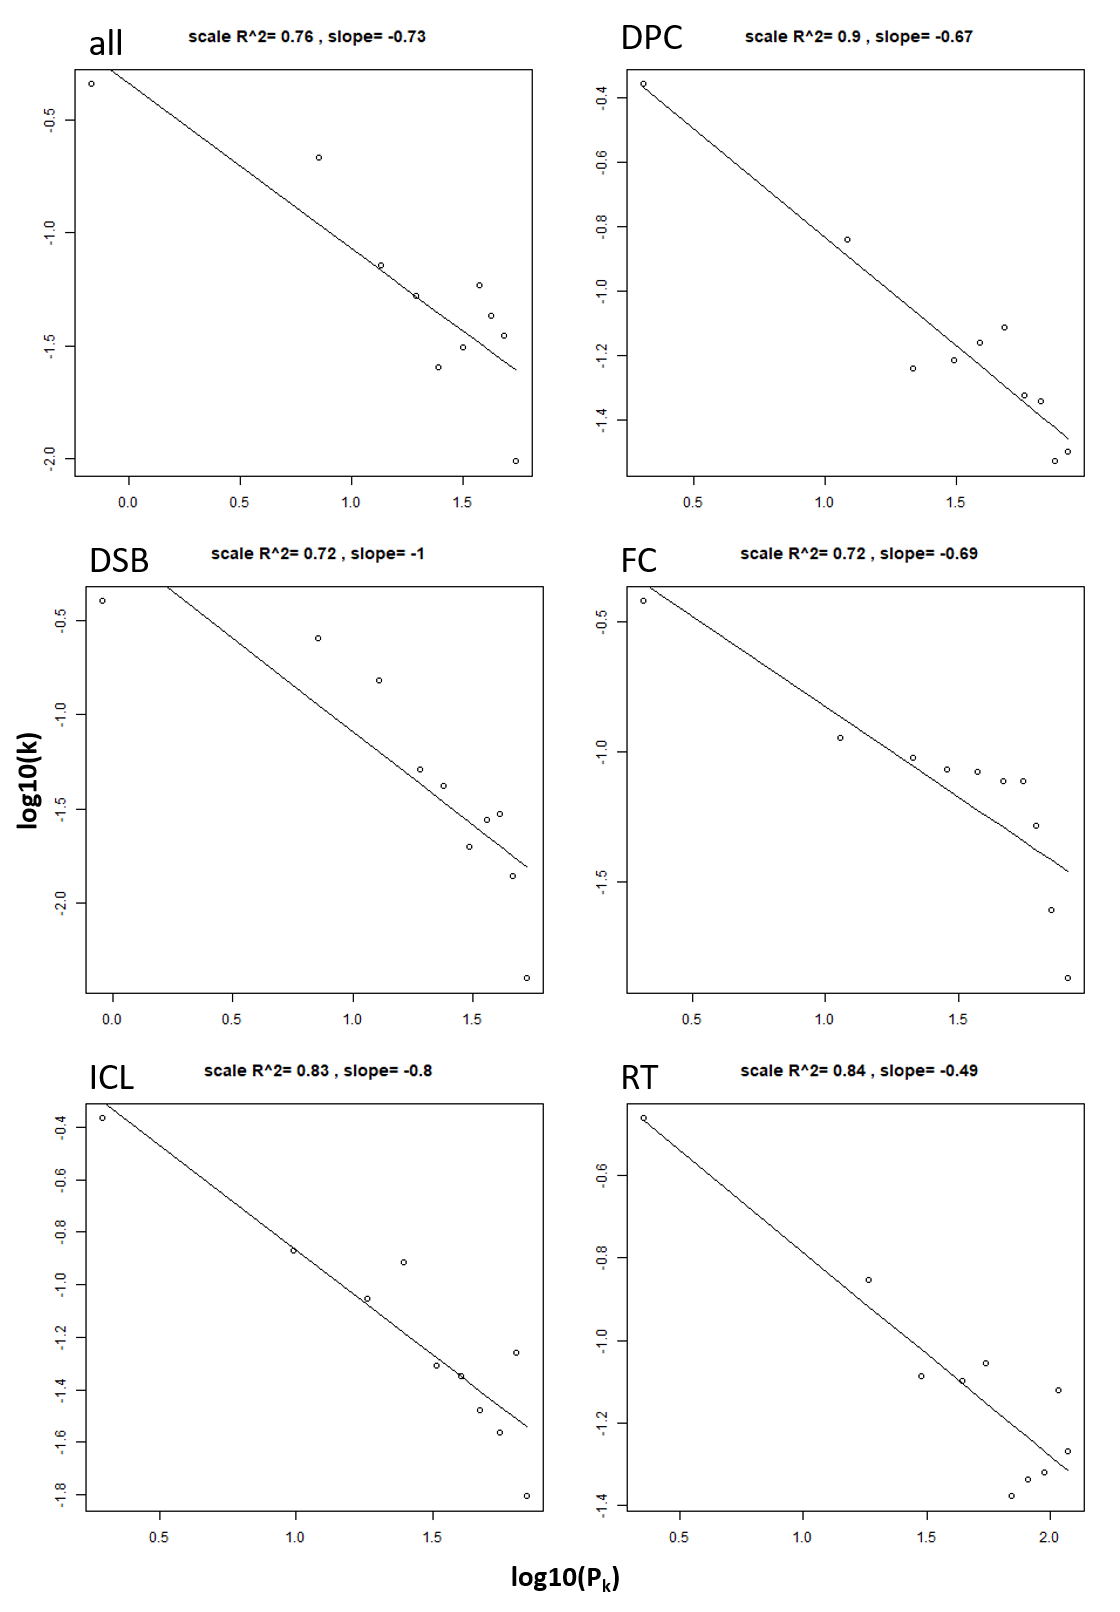
\includegraphics[width=\textwidth]{resources/images/Results/scaleFreePage.png}
    \caption[Scale free plots for all newly constructed TOM networks]{\textbf{Scale free plots for all newly constructed TOM networks. }Plotting of scale free plots was done using the a built-in function of the WGCNA package and native R methods.}
    \label{fig:scaleFreeness}
\end{figure}
If a network is scale free its node degree distribution should follow a power law which is indicated in these logarithmic plots as a linear model. The slope of this model is not really relevant for our observation of scale-freeness but the regression coefficient value shown above each plot indicates how well the networks follow the power law. Networks with an regression coefficient of above 0.6 can be considered scale free in the biological context due to real scale-freeness being very rare in real life data \citep{Broido.2019}. Given these thresholds all of our TOM networks can be considered to be scale free (see Figure \ref{fig:scaleFreeness}). Networks that do not fit this criterion can of course still be used for clustering algorithms but can yield less reliable results because they do not follow the small world principle of sufficient connectivity between all network nodes.
\begin{figure}[H]
    \centering
    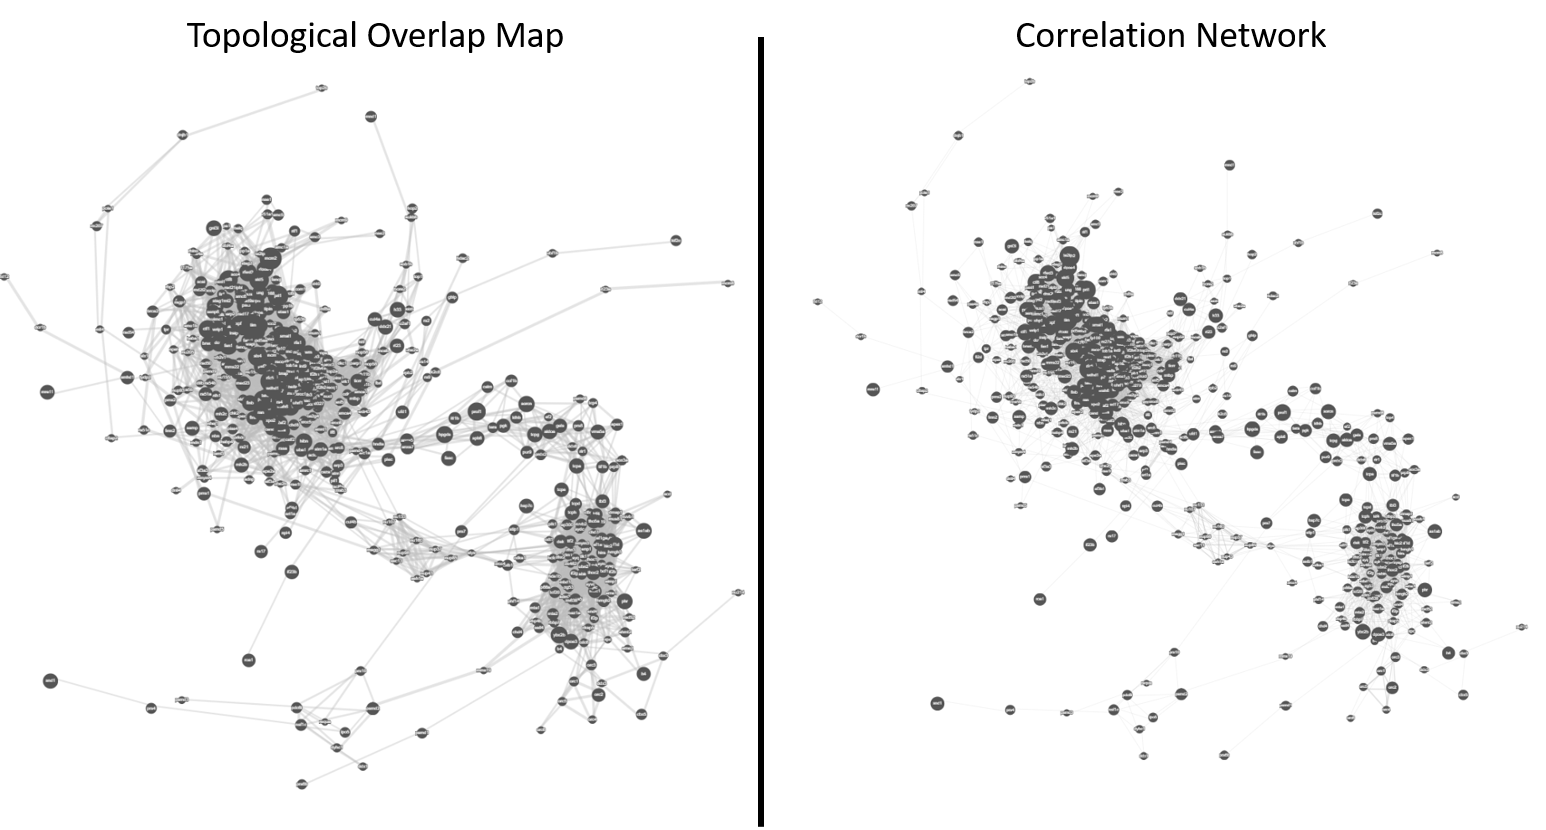
\includegraphics[width=\textwidth]{resources/images/Results/sim_tom_icl.png}
    \caption[Comparison of a Pearson Correlation Network and the respective Topological Overlap Map]{\textbf{Comparison of a Pearson Correlation Network and the respective Topological Overlap Map. } The topological overlap map and correlation network for all ICL sets were plotted next to each other. One has to note that the edges of the correlation network are unfiltered while the TOM is filtered using a soft threshold defined as $theta = 0.7 * EdgeWeight_{max}$. These two networks exist to visualize the difference between TOM and correlation and are based on a filtered protein list. They do not represent the networks that can be browsed on the DRA itself.}
    \label{fig:tomvscor}
\end{figure}
\newpage
Given the filtered nature of the TOM compared to the correlation network one can say that TOM represents protein co-regulation on a broader scale. If the correlation network were to be filtered by the same criteria, only about 50 nodes would remain in the final network. This is of course not sufficient for effective clustering and especially not useful for the identification of novel co-regulations or interactions. Generally it seems that TOMs expand the correlation network to a point where normally removed nodes are still included. Therefore it retains more information about the actual co-regulations of repair proteins. The implemented clustering algorithms of the DRA work on unfiltered versions of each networks to maximize the available data and greatly improve the ability to mine data. Due to the mentioned reasons we did not include raw correlation or adjacency networks except for the already existing curated networks.\\
To improve 
The networks constructed were then further processed depending on the needs of the user of the DRA. They can either be plotted and browsed or used as a base for Nearest Neighbor Clustering or a Diffusion algorithm to find functional clusters within the network as shown in Figure \ref{fig:co-expression} on the example of gene co-expression.
\begin{figure}[H]
    \centering
    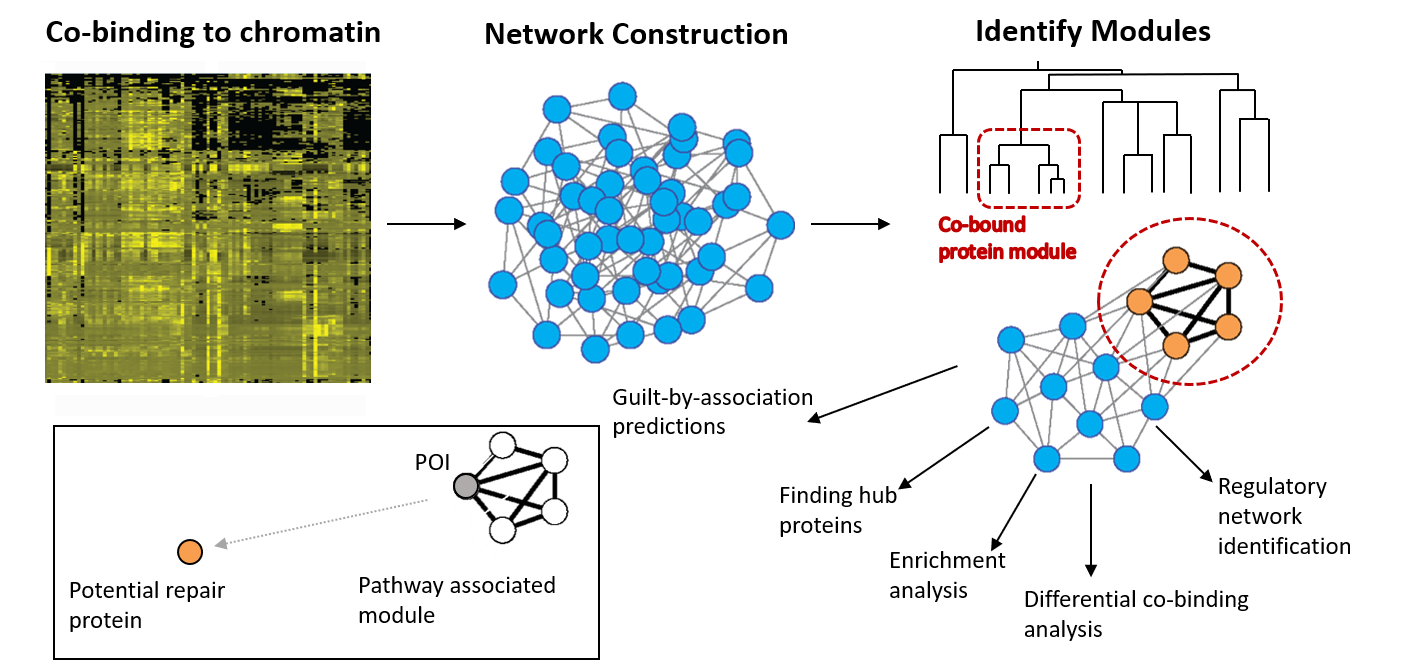
\includegraphics[width=.98\textwidth]{resources/images/Intro/co-expression.png}
    \caption[Schematic of co-binding analysis]{\textbf{Schematic of co-binding analysis. }Schematic of the steps used in co-binding analysis. Pairwise correlation is used to determine the relationship between each possible pair. This is followed by filtering of said relationships in alignment with appropriate thresholds and the visualization the remaining correlation values in form of a network. This network is then used to identify functional modules using grouping methods such as hierarchical clustering. From these modules hubs and regulating factors as well as functional predictions can be drawn. The latter can be based on the "Guilt-by-association" approach (GBA, highlighted) that identifies the function of unknown variables by the variables they cluster with. Gene co-binding is generally mathematically analogous to the protein co-regulation studied in this thesis.\\\cite{vanDam.2018}, modified}
    \label{fig:co-expression}
\end{figure}
With the created network tables using TOM as a measure of the similarity between chromatin binding behavior of repair and replication proteins it is now possible to apply clustering algorithms such as Diffusion based Network Propagation to identify functional DNA repair modules for all sets and for each DNA lesion individually. To ensure that a maximum amount of data is available to the Nearest Neighbor- and Diffusion clustering algorithms we calculated TOM maps for all DNA lesion sets including all proteins found in each run ($N_{max}=4313$). Those edge lists are only available to the clustering algorithms and can not be plotted as networks on the DRA itself. Scale-freeness for these networks was analyzed as explained above and can the corresponding plots can be seen in the supplementary collection on Github.


\subsection{Using TOM networks and Diffusion clustering to identify functional modules}
In addition to the previously included reference network consisting of 295 known DNA repair and replication proteins we now included DNA lesion specific repair networks based on topological overlap measures for DNA-Protein Crosslinks (DOC), Doublestrand Breaks (DSB), Interstrand Crosslinks (ICL), Replication Fork Collapse (FC) as well as a network visualizing protein involvement in Replication Termination (RT). These networks can be visualized using the JavaScript package cytoscape.js on demand including only the 1737 most abundant proteins under damage conditions. In addition to the processing steps mentioned in Section \ref{sec:netprocessing} a soft threshold for plotting is applied to the raw edge list before plotting. The back-end is configured in such a way that it only plots edges that have a weight higher than $0.7 * EdgeWeight_{max}$ to improve plotting performance.\\
When visualizing the networks one has to consider that each network is based on a specific set of experiments using different methods, DNA templates and especially treatments that can greatly influence the appearance and accessibility of a network plot itself. We've already mentioned that not all of the unfiltered networks can follow the scale free principle. Especially networks created from a small list of conditions and that therefore had less information available to the correlation- and TOM algorithms are very interconnected. Even though all our networks fit our criteria for biological scale free-like networks we see large differences in the plotted filtered networks (see Figures \ref{fig:DPCtom} through \ref{fig:RTtom}) with especially the ICL and DPC networks being relatively inaccessible to the users naked eye. We defined accessibility of a network as the ability of a trained user to distinguish groups of functionally similar proteins in the network plot solely by means of observation.\\ Before starting to mine the constructed networks for functional protein modules we determined that the algorithm parameters should be set to $iter = 1000000$ and $reset = 0.25$ while the number of proteins to be plotted after diffusion varies for each query. These parameters gave us results representing known modules with a great balance between computation time and accuracy.


\subsubsection{Analysis of the DNA-Protein Crosslink Network}
\label{sec:dpcnet}
\begin{figure}[H]
    \centering
    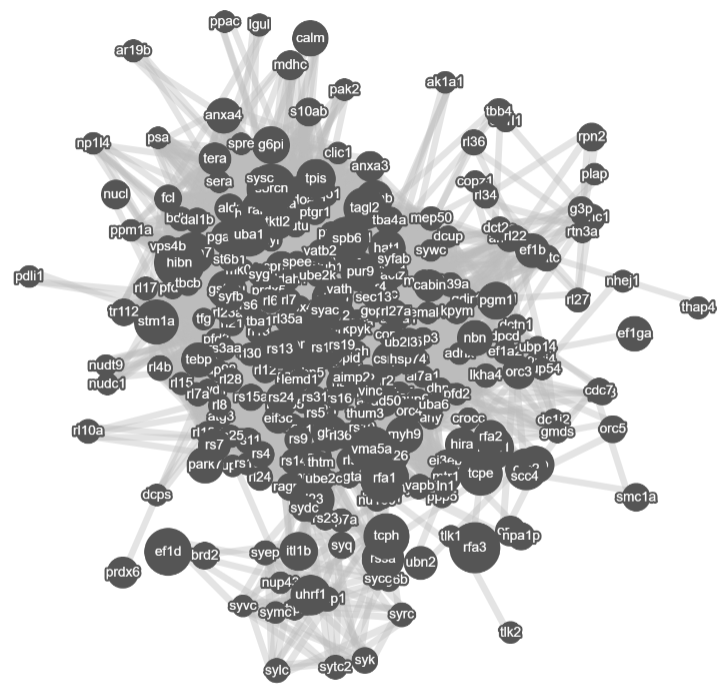
\includegraphics[width=.6\textwidth]{resources/images/Results/DPC_networkplot.png}
    \caption[DNA-Protein Crosslink TOM Network]{\textbf{DNA-Protein Crosslink TOM Network. }Depicted is the visual representation of proteins loaded onto chromatin under DNA-Protein Crosslink conditions. Edges are filtered using a soft threshold of 70\% and their width  is proportional to their score. Node size represents the protein enrichment scores.}
    \label{fig:DPCtom}
\end{figure}
As mentioned in the introduction of this work DNA-Protein Crosslinks are mostly repaired in a replication dependent manner through mechanisms that are mediated by the proteasome and the metalloprotease SPRTN. Using the network shown in Figure \ref{fig:DPCtom} one can observe replication factors on the outer right and bottom parts of the network as well as many subunits of the proteasome in the center that are grouped together. Due to the soft threshold applied for plotting SPRTN is not included in the network plot but is still available for the diffusion algorithm. To investigate whether the unfiltered network used for clustering represents published protein interactions and DNA binding mechanisms in DNA-Protein Crosslink repair we used SPRTN, PCNA and the MCM helicase as a query for the diffusion algorithm. Plotting the 20 best results yielded us the cluster shown in \ref{fig:sprtn_cluster}.\\
\begin{figure}[H]
    \centering
    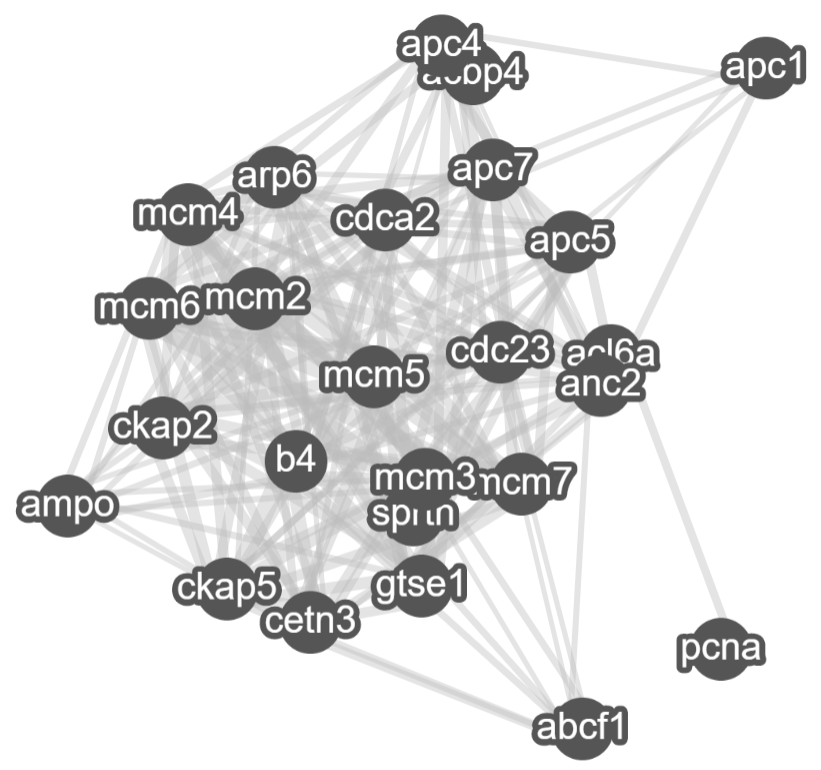
\includegraphics[width=0.5\textwidth]{resources/images/Results/sprtn_mcm_pcna_diffusion.PNG}
    \caption[Diffusion result for SPRTN and repliation associated proteins under DPC conditions]{\textbf{Diffusion result for SPRTN and repliation associated proteins under DPC conditions. }Shown is the resulting cluster graph of the diffusion algorithm based on the unfiltered DPC network.\\Query: SPRTN, PCNA, MCM2-7; 20 nodes}
    \label{fig:sprtn_cluster}
\end{figure}
This diffusion output validated that the subunits of the MCM helicase have a high similarity over all conditions of the DPC experiment series. Additionally, they seem to have a highly similar chromatin binding profile to PCNA and other DNA replication factors and checkpoint proteins such as CDC23 and CDCA2. Interestingly there is no direct edge between PCNA and SPRTN despite \cite{Vaz.2016} showing that SPRTN binds directly to the replication fork where PCNA is always loaded during replication. 
This could be an artifact of the experimental setup which relied on only two time points for the untreated control whereas five time points were measured under DNA-Protein Crosslink conditions. These differences in the setup between each condition can, as mentioned, heavily influence the performance of similarity measures such as TOM due to the fact that the correlation matrix those measures are based on make the assumption of equally distributed observations over all conditions which was not the case here.\\
Also noticeable is the lack of the SPRTN interactor p97, an ATPase that forms a dimer with Cdc48p and is involved in DPC repair \citep{Larsen.2019,Woodman.2003}. 
\begin{figure}[H]
    \centering
    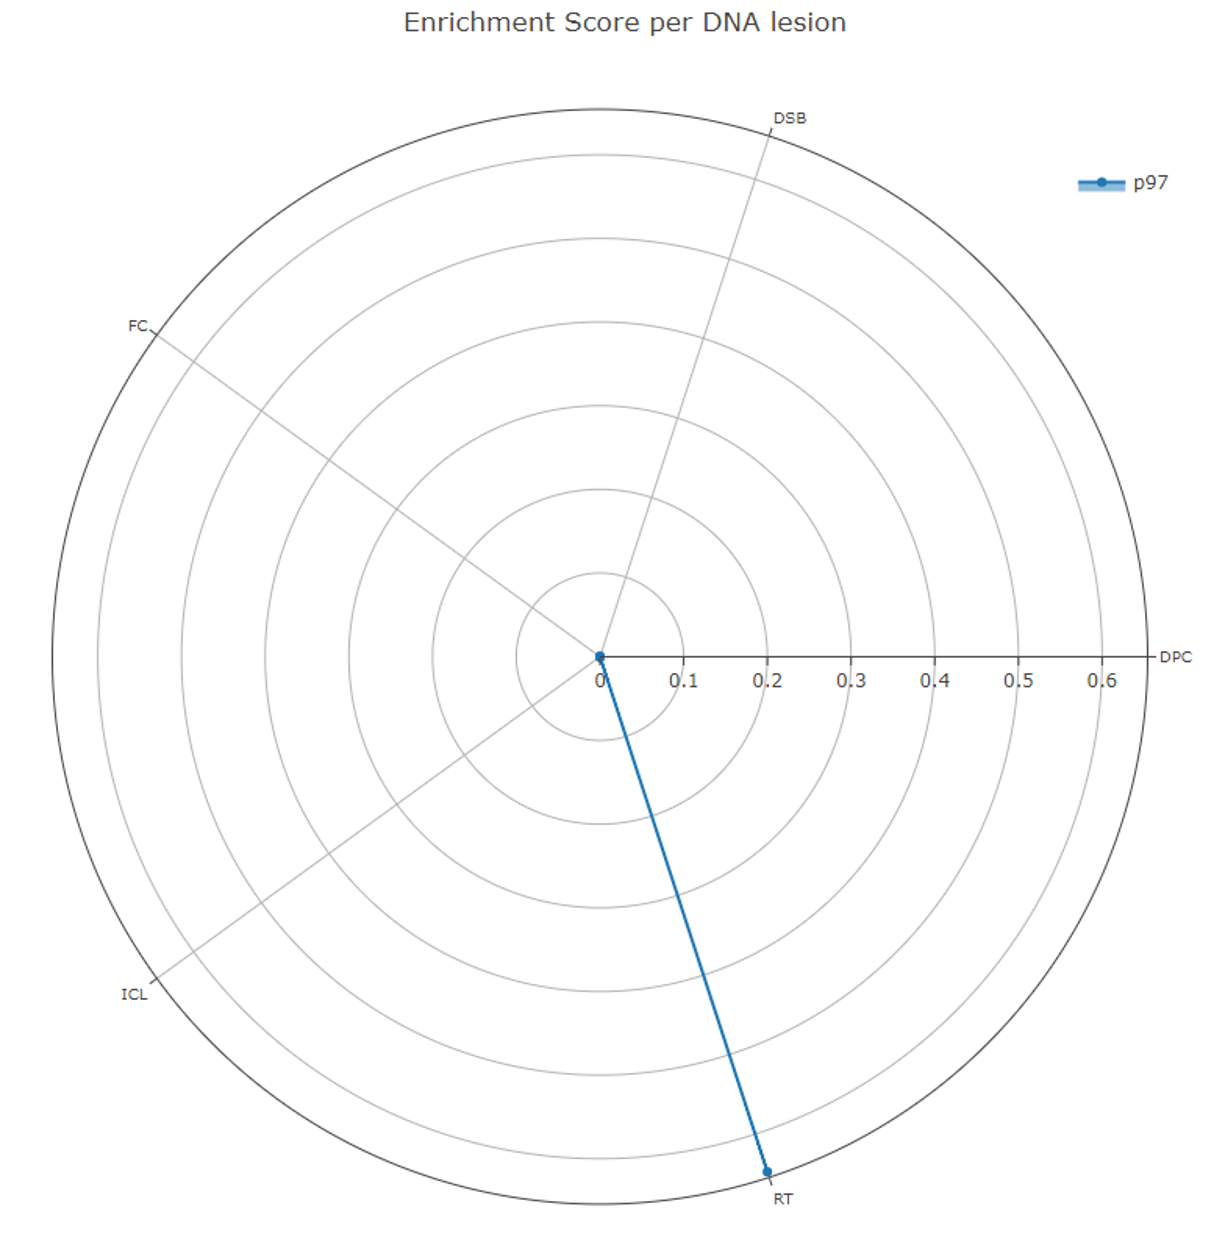
\includegraphics[width=.5\textwidth]{resources/images/Results/p97_enrichment.png}
    \caption[Enrichment of p97 over all DNA lesion types]{\textbf{Enrichment of p97 over all DNA lesion types. }Shown are the enrichment scores for p97 over all DNA lesion types. p97 only has a score for Replication Termination suggesting it has not been measured in any other set in a significant abundance.}
    \label{fig:p97dpc}
\end{figure}
Digging deeper through the data one can find that p97 has not been detected in the sets used to create the DSB network (see Figure \ref{fig:p97dpc}) which can be expected given the use of pure non-replicating HSS. p97 should be only introduced to the system once NPE is added.


\subsubsection{Analysis of the Doublestrand Break Network}
\label{sec:dsbnet}
\begin{figure}[H]
    \centering
    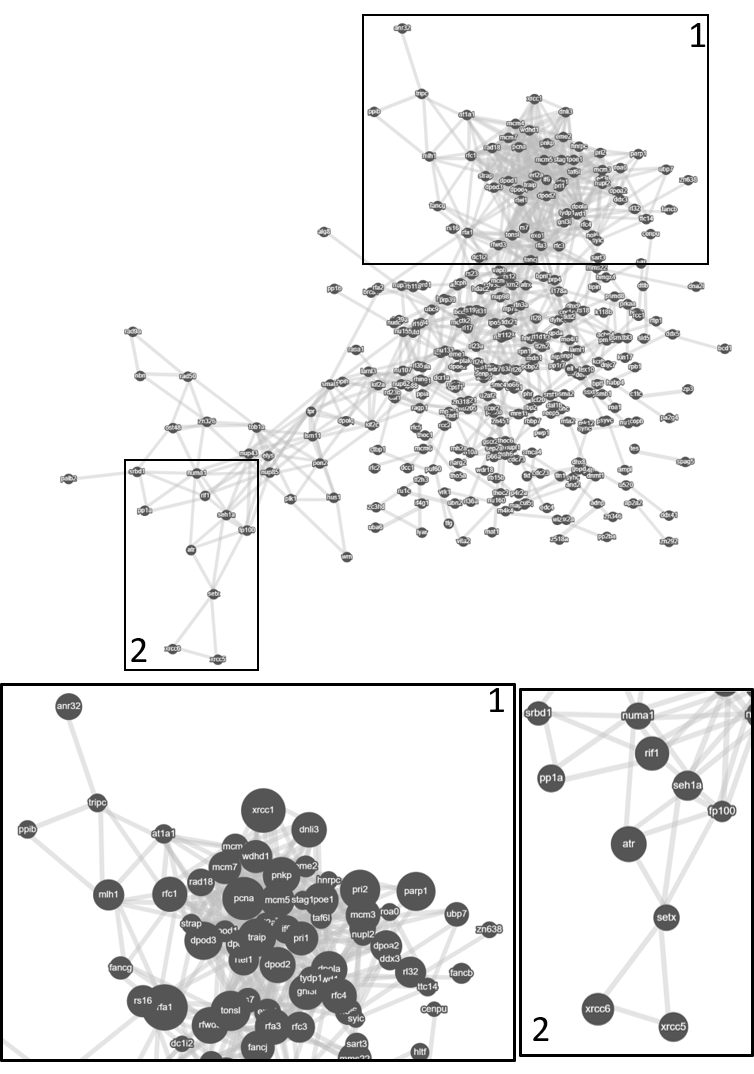
\includegraphics[width=.8\textwidth]{resources/images/Results/DSB_networkplot.png}
    \caption[Doublestreand Break TOM Network]{\textbf{Doublestreand Break TOM Network. }Visual representation of proteins loaded onto chromatin under Doublestrand Break conditions. Edges are filtered using a soft threshold of 70\% and their width  is proportional to their score. Node size in zoomed windows represents the protein enrichment scores.}
    \label{fig:DSBtom}
\end{figure}
In contrast to all other networks looked at in this work the DSB network used experiment sets only collected using HSS meaning that this network depicts replication independent DSB repair. Proteins associated with replication initiation and origin licensing will be found in the set but replication firing could not occur. As can be seen in Figure \ref{fig:DSBtom} the Doublestrand Break network shows groups of proteins that are distinguishable by means of observation. The network itself feature a low number of nodes with diverse degrees. Looking at the top right (labeled \textbf{1}) group of proteins one can make out proteins associated with origin licensing (Section \ref{sec:cellcycle}) and the formation of a pre-RC as well as the first polymerases with missing co-factors. Additionally, the E3 ubuquitin ligase TRAIP is closely connected to PCNA indicating the successful detection of DNA damage. In the bottom left of the network another high scoring group of proteins including ATR and the DSB repair factors XRCC5 and XRCC6 can be seen. This network represents mechanisms of DSB repair fairly well even in its filtered form for plotting. To see whether full DSB repair modules can be identified we used the known repair factors ATR, ATM, TRAIP, XRCC5 and XRCC6 as the query for our diffusion algorithm and plotted the 30 highest scoring proteins in Figure \ref{fig:atratm_diff}.
\begin{wrapfigure}{r}{0.5\textwidth}
    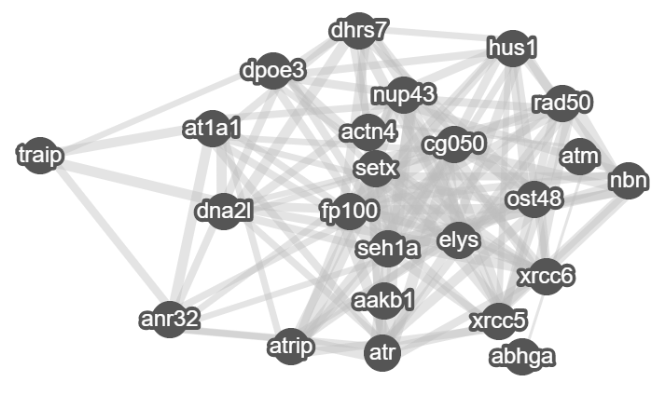
\includegraphics[width=0.46\textwidth]{resources/images/Results/dsb_diff_atratm.PNG}
    \caption[Diffusion result for ATR, ATM and other DSB repair proteins under DSB conditions]{\textbf{Diffusion result for ATR, ATM and other DSB repair proteins under DSB conditions. }Shown is the resulting cluster graph of the diffusion algorithm based on the unfiltered DSB network.\\Query: ATR, ATM, TRAIP, XRCC5, XRCC6; 30 nodes}
    \label{fig:atratm_diff}
\end{wrapfigure}
As \cite{Cimprich.2008} showed in their review on the function ATR in maintaining genome integrity the replication independent repair of DSBs works in two ways. The first mechanisms detects ssDNA by RPA binding which in turn leads to ATR/ATRIP recruitment as well as the loading of the 9-1-1 complex (Rad9-Hus1-Rad1) onto the first available dsDNA section after the DSB. This method is reflected in the lower part of the cluster seen on the right. The right side of the cluster represents the detection and repair of double stranded ends via ATM and the following recruitment of RAD50.\\
To further show how robust the DSB network is in representing protein recruitment profiles we used the MCM helicase subunits MCM2-7 as an input for Diffusion and plotted the 15 highest scoring proteins the result of which can be seen in Figure \ref{fig:diff_mcm_dsb}. It shows a closed cluster of all MCM subunits as well as the DNA polymerases (Pol\textdelta~ and Pol\textalpha) expected on licensed chromatin. Additionally the SMC5/6 loading factor Slf1  (as ANR32; \cite{Raschle.2015}) is depicted as behaving similar to MCM4, 5 and 7 as well as Pol\textdelta~ subunit 1. 
\begin{figure}
    \centering
    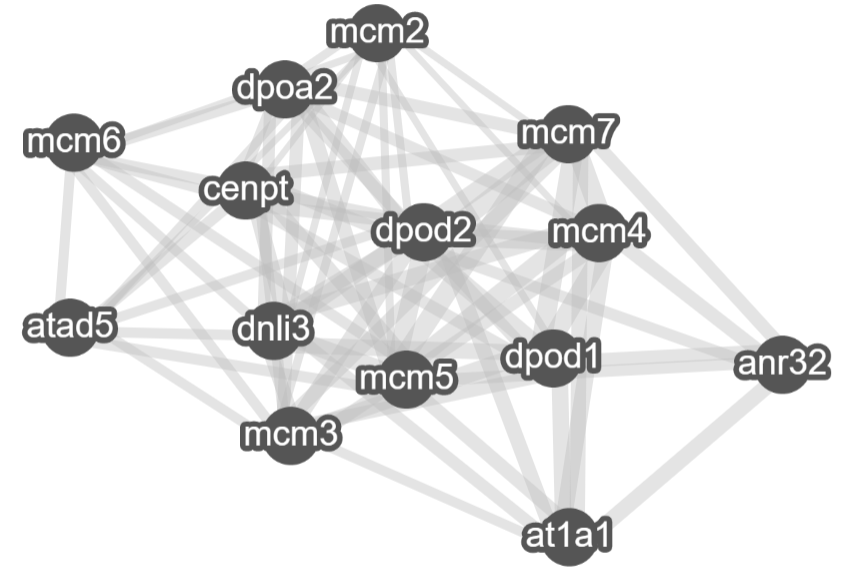
\includegraphics[width=.5\textwidth]{resources/images/Results/diff_mcm_dsb.PNG}
    \caption[Diffusion result for the MCM helicase]{\textbf{Diffusion result for the MCM helicase. }Shown is the resulting cluster graph of the diffusion algorithm based on the unfiltered DSB network.\\Query: MCM2-7; 15 nodes}
    \label{fig:diff_mcm_dsb}
\end{figure}
This result suggests that the newly deployed DSB TOM network represents the recruitment of DSB repair proteins as well as the processes of chromatin licensing and the formation of the pre-RC in non-replicating extracts.\newpage
\subsubsection{Analysis of the Replication Fork Collapse network}
\begin{figure}[H]
    \centering
    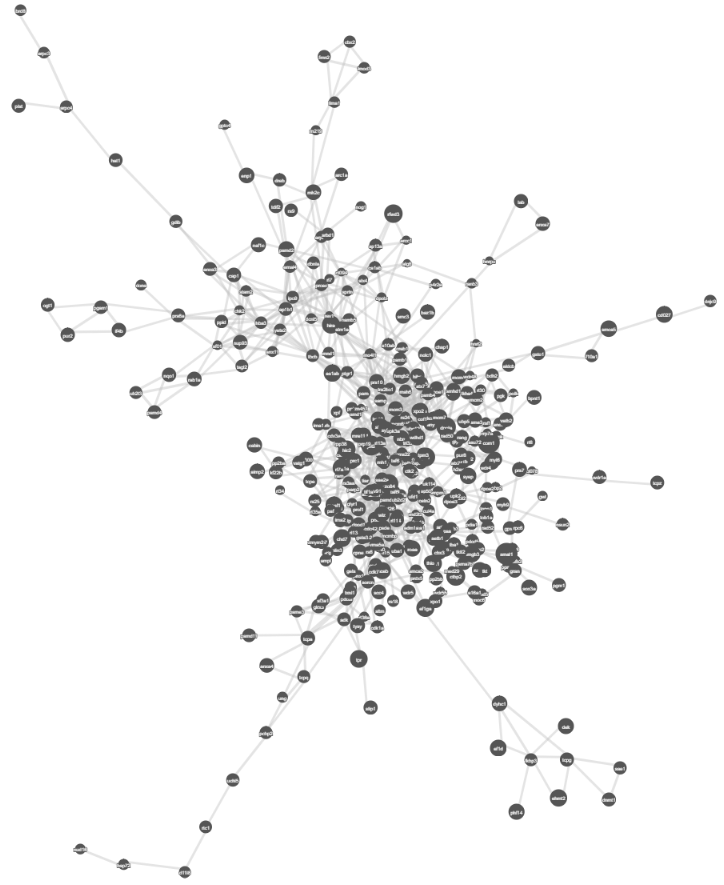
\includegraphics[width=.8\textwidth]{resources/images/Results/FC_networkplot.png}
    \caption[Fork Collapse TOM Network]{\textbf{Fork Collapse TOM Network. }Visual representation of proteins loaded onto chromatin during Replication Fork Collapse. Edges are filtered using a soft threshold of 70\% and their width  is proportional to their score. Node size in zoomed windows represents the protein enrichment scores.}
    \label{fig:FCtom}
\end{figure}
During the replication of DNA the replisome encounters many obstacles such as DNA damages or sequences that are difficult to replicate. These obstacles can cause fork stalling that may lead to the collapse of the fork itself by replisome disassembly. In his review \cite{Cortez.2015} describes how the replication checkpoint prevents replication fork stalling for example via the regulation of helicases like BLM, nucleases like DNA2 and EXO1 and translocases like SMARCAL1 via ATR.
All of the mentioned enzymes fulfill roles in different repair mechanisms but all have in common that they are involved in fork regression or fork reversal (see Section. \ref{sec:polblock}). The result of using these enzymes as a query to diffuse over the unfiltered Fork Collapse network can be seen in Figure \ref{fig:atrtarget_diff_fc}.
\begin{wrapfigure}{r}{0.5\textwidth}
    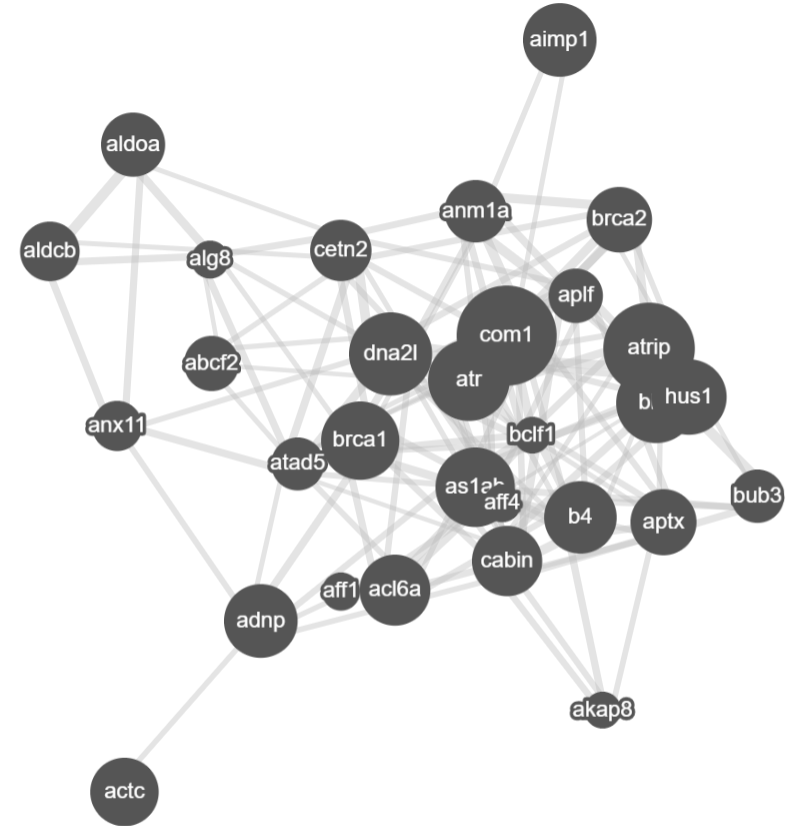
\includegraphics[width=0.46\textwidth]{resources/images/Results/fc_atrtargets.PNG}
    \caption[Diffusion result for ATR, BLM, DNA2 and SMARCAL1 under Fork Collapse conditions]{\textbf{Diffusion result for ATR, BLM, DNA2 and SMARCAL1 under Fork Collapse conditions. }Shown is the resulting cluster graph of the diffusion algorithm based on the unfiltered DSB network.\\Query: ATR, BLM, DNA2(DNA2L), SMARCAL1 (HUS1); 30 nodes}
    \label{fig:atrtarget_diff_fc}
\end{wrapfigure}
The highest node with the highest diffusion score within the resulting cluster is ATR indicating that it connects most of the found nodes with another and therefore could play a crucial role in their recruitment or function. As is already known, direct targets of ATR are involved in fork reversal suggesting that the FC-TOM network represents the mechanism of fork collapse well. On the right side of the cluster one can see the translocase HUS1 (SMARCAL1) in close vicinity to the helicase BLM and ATRIP, the ATR interacting protein. These targets of ATR are closely connected to the high scoring repair proteins BRCA1, BRCA2 and APTX (XRCC1) that were also present and enriched in experiments investigating the replication-independent repair of DSBs (see Section \ref{sec:dsbnet}). Given the fact that double- and singlestrand breaks are a common cause of replication fork stalling and also a result of proteasome dissociation \citep{Cortez.2015} the inclusion and high diffusion- and enrichment scores for these factors is expected. 



\subsubsection{Analysis of the Interstrand Crosslink network}
\label{sec:iclnet}
The Interstrand Crosslink network is built on the person correlation based TOM of NPE/HSS using Psoralen-treated sperm chromatin. Under Psoralen treatment interstrand crosslinks are introduced at random into the chromatin template and mostly repaired via the Fanconi Anemia (FA) pathway. The mechanism of ICL bypass and repair in \textit{Xenopus} egg extracts has been resolved in high detail by \cite{Raschle.2015}. Replication of Psoralen-treated chromatin starts with the loading of all necessary replication proteins followed by triggering a transient checkpoint response. After encountering an ICL replicative DNA polymerases are unloaded while TLS polymerases as well as the entire Fanconi core complex are loaded. Additionally the nucleases XPX and FAN1 are loaded together with the FA core complex that is loaded by a ubiquitylated FANCD2/FANCI dimer \citep{Raschle.2015,Knipscheer.2009,Raschle.2008}.
\begin{figure}[H]
    \centering
    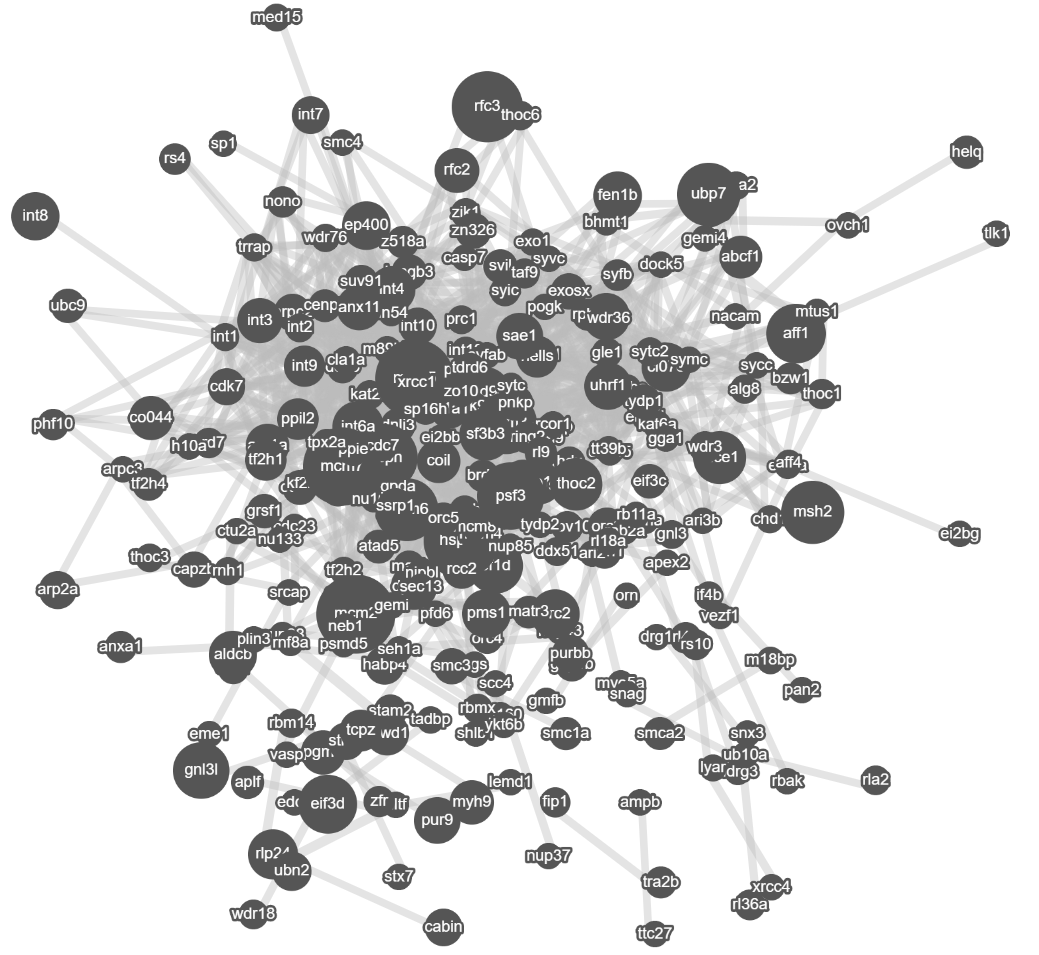
\includegraphics[width=\textwidth]{resources/images/Results/ICL_networkplot.PNG}
    \caption[Interstrand Crosslink TOM Network]{\textbf{Interstrand Crosslink TOM Network. }Visual representation of proteins loaded onto chromatin under Interstrand Crosslink conditions. Edges are filtered using a soft threshold of 70\% and their width  is proportional to their score. Node size in zoomed windows represents the protein enrichment scores.}
    \label{fig:ICLtom}
\end{figure}
Using the FA core complex as the query to diffuse over the ICL network we expected to find most repair enzymes as well as TLS polymerases in the resulting cluster.
\begin{wrapfigure}{l}{0.5\textwidth}
    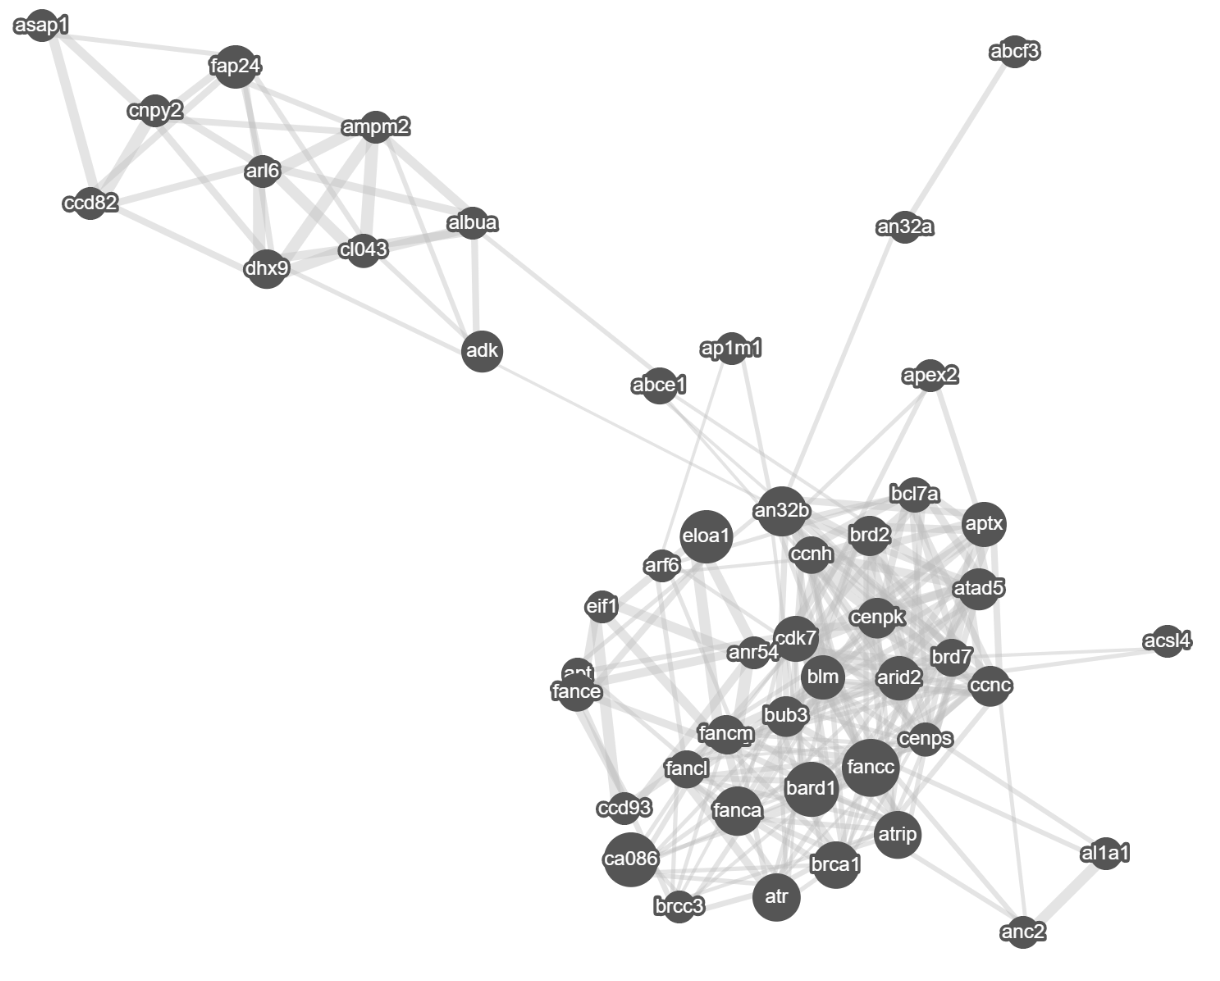
\includegraphics[width=0.46\textwidth]{resources/images/Results/FAcore_diff_ICL_50.PNG}
    \caption[Diffusion result for the Fanconi core complex under Interstrand Crosslink conditions]{\textbf{Diffusion result for the Fanconi core complex under Interstrand Crosslink conditions. }Shown is the resulting cluster graph of the diffusion algorithm based on the unfiltered DSB network.\\Query: GO:0043240; 50 nodes}
    \label{fig:atrtarget_diff_fc}
\end{wrapfigure}
Surprisingly, of the FA loading complex dimer only FANCI could be detected. Otherwise all proteins of the FA core complex are closely connected to the helicase BLM as well as ATR and BRCC3. The latter is a subunit of an E3 ubiquitin ligase which is involved in the recruitment of BRCA1 to DNA lesions. BRCA1 is also found in the resulting cluster being a direct neighbor to FANCC and FANCA as well as ATRIP and ATR. Given the slightly shifted peaks of FA and its recruiters as well as the TLS polymerases and FA itself it is possible that the proteins expected to be included in the first cluster are not in the list of 50 highest scoring neighbor nodes we defined. Outputting a cluster consisting of 100 nodes for example will not be plotted because the server takes to long to answer the users request and the script runs into a hard coded timeout that can not be changed.\\
To circumvent this problem we repeated the diffusion using the FA recruiter FANCD2 and POL\textkappa, a TLS polymerase, as the query proteins and plotting the 50 highest scoring proteins. Approaching the search for ICL repair related proteins from the angle of known regulatory proteins resulted in the expected group of proteins. 
\begin{figure}[H]
    \centering
    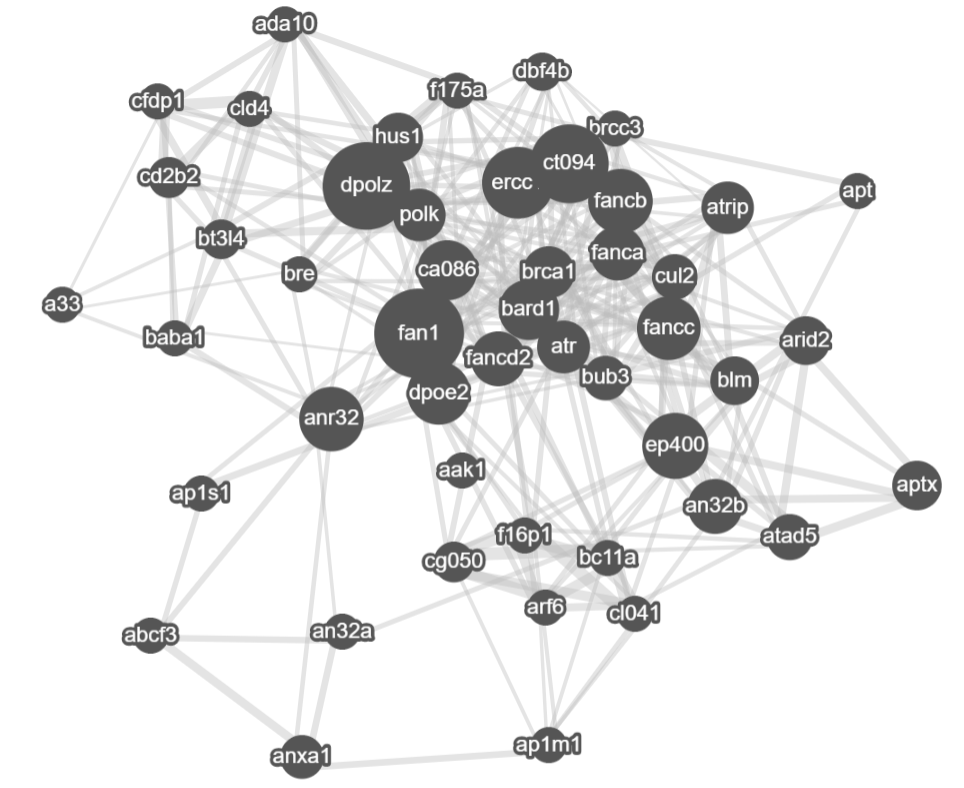
\includegraphics[width=0.5\textwidth]{resources/images/Results/icl_diff_fancd2_polk.PNG}
    \caption[Diffusion result for FANCD2 and POL\textkappa~ under Interstrand Crosslink conditions]{\textbf{Diffusion result for the Fanconi core complex and its recruiters under Interstrand Crosslink conditions. }Shown is the resulting cluster graph of the diffusion algorithm based on the unfiltered DSB network.\\Query: FANCD2, POL\textkappa; 50 nodes}
    \label{fig:icl_diff_fancd2_polk}
\end{figure}
Using FANCD2 and POL\textkappa~ to diffuse over the ICL network yielded a cluster of highly enriched enzymes known to be involved in ICL repair. Aside from the DNA binding subunits of the FA core complex (FANCA and FANCB) the repair associated helicase BLM was found in direct neighborhood of FANCC together with ATR and BRCA1 as it was the case for the diffused cluster using the FA core complex. Other enzymes involved in doublestrand break repair such as HUS1 and ATRIP are also part of the cluster which is to be expected considering that it is possible for ICLs to be bypassed using a combination of translesion synthesis and doublestrand break repair (see Section \ref{sec:iclrepair} for details). Another highly enriched protein included in the cluster is FAN1 which is a nuclease found to be associated with the FA core complex and FANCD2 thought to act together with MUS81 cut covalently crosslinked DNA \citep{ODonnell.2010}. Another interesting protein in the cluster is DPOLZ (also known as REV3), the catalytic subunit of DNA polymerase zeta. It is known to be involved in DNA repair, especially in the replication-dependent resolution of doublestrand breaks and therefore it plays a major role in bypassing covalent ICLs \citep{Raschle.2008} as REV3 depleted \textit{Xenopus} egg extracts have been shown to be ICL repair deficient \citep{Raschle.2008}.

\subsubsection{Analysis of the Replication Termination network}
\begin{figure}[H]
    \centering
    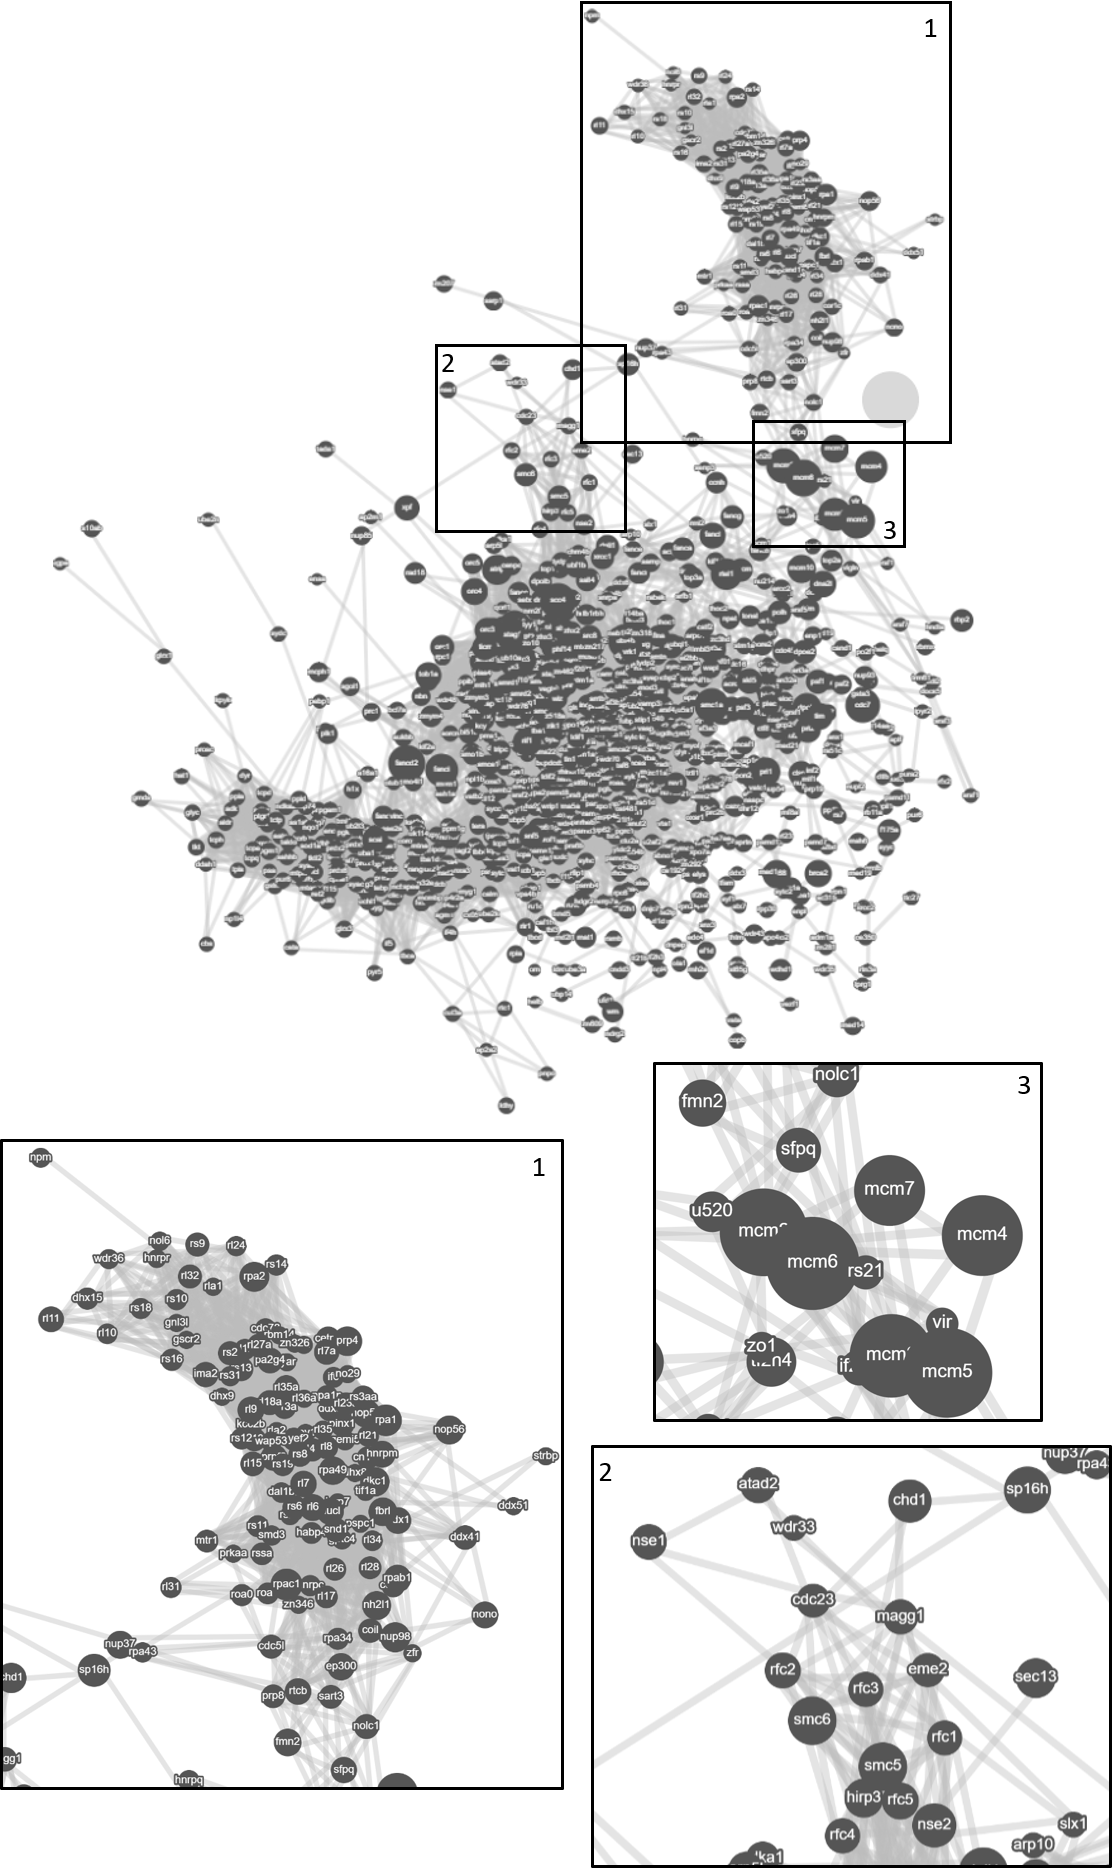
\includegraphics[width=.7\textwidth]{resources/images/Results/RT_networkplot.png}
    \caption[Replication Termination TOM Network]{\textbf{Replication Termination TOM Network}. Visual representation of proteins loaded onto chromatin during Replication Termination. Edges are filtered using a soft threshold of 70\% and their width  is proportional to their score. Node size in zoomed windows represents the protein enrichment scores.}
    \label{fig:RTtom}
\end{figure}

\subsection{The benefits of using individual damage networks over combined network representation}


\newpage
\section{Discussion}\label{sec:discussion}
\newpage
\section{Acknowledgement}

\newpage
\section{Literature}
\bibliography{masterthesis}
\newpage
\newpage

\end{document}
